\chapter{Experimentos y resultados}
\label{ch:results}

En este capítulo presentaremos los experimentos principales realizados a partir
de lo desarrollado en el capítulo \ref{ch:method}. Entrenaremos 2 grupos de
modelos predictivos. Un grupo con una codificación ad-hoc, y otro grupo con una
codificación por word embeddings. Los vectores de características tendrán como
información una ventana del plan relajado y una acción. Se destacarán aquellos
modelos que presenten mejores resultados en validación cruzada y sobre ejemplos
del conjunto de test. Para aquellos modelos que tuvieron un mal desempeño,
mencionaremos algunas de las posibles causas.

Por otro lado se entrenarán los 3 algoritmos de clasificación vistos en el
capítulo \ref{ch:lit_ml}, \emph{XGBoost}, \emph{regresión logística}, y
\emph{perceptrón multicapa}. Los conjuntos de entrenamiento y de test son
divididos por esquemas de acción, entrenando un modelo por cada uno. Esto con el
fin de capturar la información significativa de un solo esquema por modelo. En
resumen, la estructura de nuestros experimentos para ambos grupos es la
siguiente:

\begin{itemize}
    \item Codificación ad-hoc o por word embeddings:
    \begin{itemize}
        \item Regresión logistica:
        \begin{itemize}
            \item \verb|take_image|
            \item \verb|turn_to|
            \item \verb|calibrate|
            \item \verb|switch_on|
            \item \verb|switch_off|
        \end{itemize}
        \item XGBoost:
        \begin{itemize}
            \item \verb|take_image|
            \item \verb|turn_to|
            \item \verb|calibrate|
            \item \verb|switch_on|
            \item \verb|switch_off|
        \end{itemize}
        \item Redes neuronales:
        \begin{itemize}
            \item \verb|take_image|
            \item \verb|turn_to|
            \item \verb|calibrate|
            \item \verb|switch_on|
            \item \verb|switch_off|
        \end{itemize}
    \end{itemize}
\end{itemize}

Esto es un total de 15 modelos por grupo. Para los mejores modelos, se
calcularon los tiempos de predicción con el fin de determinar si es viable
realizar grounding heurístico con estos modelos en el algoritmo de Fast
Downward.

Por último, mencionaremos otros experimentos que se trabajaron durante la tesis,
que a pesar de no lograr el resultado que esperábamos, fueron muy importantes
para guiar futuros experimentos.

\section{Modelos predictivos por word embeddings}
\label{exp:ad-hoc}

\subsection{Configuración del experimento}

En primer lugar, se necesito asignar la configuración para la construcción de las ventanas y planes relajados.  Observamos que
por lo general los planes relajados del conjunto de entrenamiento suelen tener
entre $3$ a $10$ acciones. Nuestro algoritmo debe ser capaz de generalizar para
ejemplos de entrenamientos no antes visto, por lo que el preprocesamiento que
realicemos sobre estos datos debe ser orientado a reducir las discrepancias
entre un ejemplo nuevo y los que fueron utilizados en la etapa de entrenamiento.
Como el largo de los planes relajados de los problemas de test es por encima de los cientos de acciones, generamos ventanas que aproximen en
en tamaño a los planes relajados de los problemas de entrenamiento. Es por ello, que optamos por un paso y tamaño de ventana de $3$.

Para el entrenamiento de los clasificadores, se realizó una búsqueda de
hiper-parámetros cuya métrica a optimizar es $H_{\beta}$ con $\beta = 1.5$. Dado
que en nuestro problema es más importante predecir correctamente todas las
acciones relevantes, optamos por priorizar la taza de verdaderos positivos sobre
la taza de verdaderos negativos. Es decir, buscamos que el clasificador sea
penalizado si no logra predecir todas las acciones relevantes para obtener un
plan, y si no logra filtrar una cantidad aceptable de acciones no relevantes.

Recordemos que para evaluar los modelos, generamos las predicciones a nivel de
ventana de plan relajado y acción. No obstante, buscamos predecir si una acción
es relevante dada la información del plan relajado completo, por lo que es
necesario agrupar las predicciones que cada ventana realizó sobre esa acción.
Por ejemplo, supongamos que tenemos $M$ ventanas de un plan relajado $\vec{a}$
de una tarea $\Pi$ y se busca determinar la probabilidad de una acción $a'$ dado
$\vec{a}$. El modelo de aprendizaje automático propuesto realiza $M$
predicciones para $a'$ dado las $M$ ventanas de $\vec{a}$ donde cada estimación
es una probabilidad. En lugar de evaluar el modelo con las $M$ predicciones, las
agrupamos para obtener solo una. Para este experimento, seleccionamos el máximo
de las $M$ probabilidades. Notar que bajo esta decisión, una probabilidad baja
significa que para todas las ventanas del plan relajado, el planificador le
asignó una baja probabilidad a $a'$, mientras que una probabilidad alta requiere
que por lo menos una ventana del plan relajado haya provisto la información
necesaria para considerar relevante a $a'$.

Por último, los algoritmos presentados en el capítulo \ref{ch:lit_ml}
implementan una solución genérica de los métodos de aprendizaje. Por lo que se
requiere especificar como van a estar configurados antes de empezar el proceso
de entrenamiento. La siguiente lista de parámetros muestra aquellos que fueron
utilizados para cada algoritmo en este experimento:

\begin{conditions}
\emph{Nombre\ del\ modelo} & \verb|Regresión logística| \\
\emph{penalty} & \verb|[elasticnet]| \\
\emph{C} & \verb|[1, 0.1, 0.01]| \\
\emph{class\_weight} & \verb|[balanced]|  \\
\emph{solver} & \verb|[saga]|  \\
\emph{max\_iter} & \verb|[1000 10000]| \\
\emph{random\_state} & \verb|[0]| \\
\emph{l1\_ratio} & \verb|[0, 1]|
\end{conditions}

\begin{conditions}
\emph{Nombre\ del\ modelo} & \verb|XGBoost| \\
\emph{objective} & \verb|[binary:logistic]| \\
\emph{n\_estimators} & \verb|[500, 1000]| \\
\emph{gamma} & \verb|[0.001, 1]| \\
\emph{max\_depth} & \verb|[10, 20]| \\
\emph{alpha} & \verb|[0.001, 1]| \\
\emph{lambda} & \verb|[0.001, 1]| \\
\emph{booster} & \verb|[gbtree]| \\
\emph{colsample\_bytree} & \verb|[1]| \\
\emph{subsample} & \verb|[0.5]| \\
\emph{eval\_metric} & \verb|[logloss]| \\
\emph{use\_label\_encoder} & \verb|[false]| \\
\emph{random\_state} & \verb|[0]|
\end{conditions}

\begin{conditions}
\emph{Nombre\ del\ modelo} & \verb|PytorchNN| \\
\emph{h\_size} & \verb|[32, 64]| \\
\emph{n\_layers} & \verb|[2, 4, 8, 16]| \\
\emph{bn\_bool} & \verb|[False]| \\
\emph{p} & \verb|[0, 0.1]| \\
\emph{epochs} & \verb|[20]| \\
\emph{batch\_size} & \verb|[32]| \\
\emph{balanced} & \verb|[True]| \\
\emph{lr} & \verb|[0.001]| \\
\end{conditions}

Estos parámetros corresponden con la interfaz provista por las librerías de
\emph{Scikit-learn} y \emph{Pytorch} que implementan los algoritmos de aprendizaje. Cada parámetro muestra una lista de 1 o más valores donde cada elemento representa una posible asignación de ese parámetro. La cantidad de configuraciones posibles de un modelo es igual al producto cartesiano de cada una de las listas de los parámetros de un modelo. Por ejemplo para el caso de la regresión
logística, los parámetros \emph{C}, \emph{max\_iter}, y \emph{l1\_ratio} tienen 3, 2, y 2 asignaciones respectivamente, el resto de parámetros solo tiene una. Por lo tanto, hay un total de $3 \times 2 \times 2 = 12$ configuraciones del modelo.

Los parámetros que seleccionamos siempre buscaban plantear variantes en la función de costo a optimizar, el tipo de optimizador, y métodos para evitar el sobreajuste. En particular, seguimos como guía valores comunes que la comunidad de aprendizaje automático suele utilizar para estos modelos,  la experiencia transmitida por el ´boca a boca´, y conocimientos tanto del área de planning como del funcionamiento interno de los modelos utilizados. 

En el caso de la regresión logística, los parámetros \emph{penalty},
\emph{l1\_ratio}, y \emph{C} permiten realizar variaciones en la regularización
de la función de costo, evitando que la norma del vector de pesos del modelo
crezca demasiado por sobreajuste. \emph{solver} indica el método de optimización de la función de costo. \emph{max\_iter} es el número
de iteraciones que requiere el algoritmo para converger. Por último,
\emph{class\_weight} permite configurar el modelo de tal manera que balancee
la cantidad de ejemplares positivos y negativos del material de entrenamiento. Este último es importante para nosotros ya que nuestro conjunto de entrenamiento está desbalanceado, teniendo una mayor cantidad de good operators que de
bad operators por problema.

XGBoost requiere que se le especifiquen la cantidad de árboles a
ensamblar con \emph{n\_estimators}, la fuerza del parámetro de regularización
\emph{gamma}, y la profundidad máxima de los árboles \emph{max\_depth}. \emph{objetive} indica la función objetivo a optimizar, en este caso la misma función de costo que una regresión logística. \emph{booster} permite seleccionar variantes del método iterativo de boosting explicado en el capítulo \ref{alg:xgboost}. Por último \emph{colsample\_bytre} y \emph{subsample} permiten
tomar una muestra con reposición de las filas o columnas en la confección de un árbol en el ensemble con el proposito de reducir el sobreajuste.

La red neuronal necesita del número de neuronas para todas las capas
\emph{h\_size}, la cantidad de capas ocultas \emph{n\_layers}, si los vectores
de entrada son normalizados \emph{bn\_bool}, y la probabilidad  \emph{p} de apagar momentáneamente neuronas de la red de manera
aleatoria.

Por cada posible asignación obtenemos aquella que mejor se comporte con el conjunto de test. Recordemos que nuestro objetivo es encontrar modelos que se pueda utilizar para algún esquema de acción. De un total de 5 esquemas de acción en el dominio \emph{Satellite}, el mejor caso sería encontrar 5 modelos que den buenos resultados en esos esquemas.

\subsection{Resultados}

Empecemos analizando el mejor modelo que llegamos a obtener para el esquema de \emph{}



\begin{figure}
    \centering
    \begin{subfigure}[b]{0.83\textwidth}
    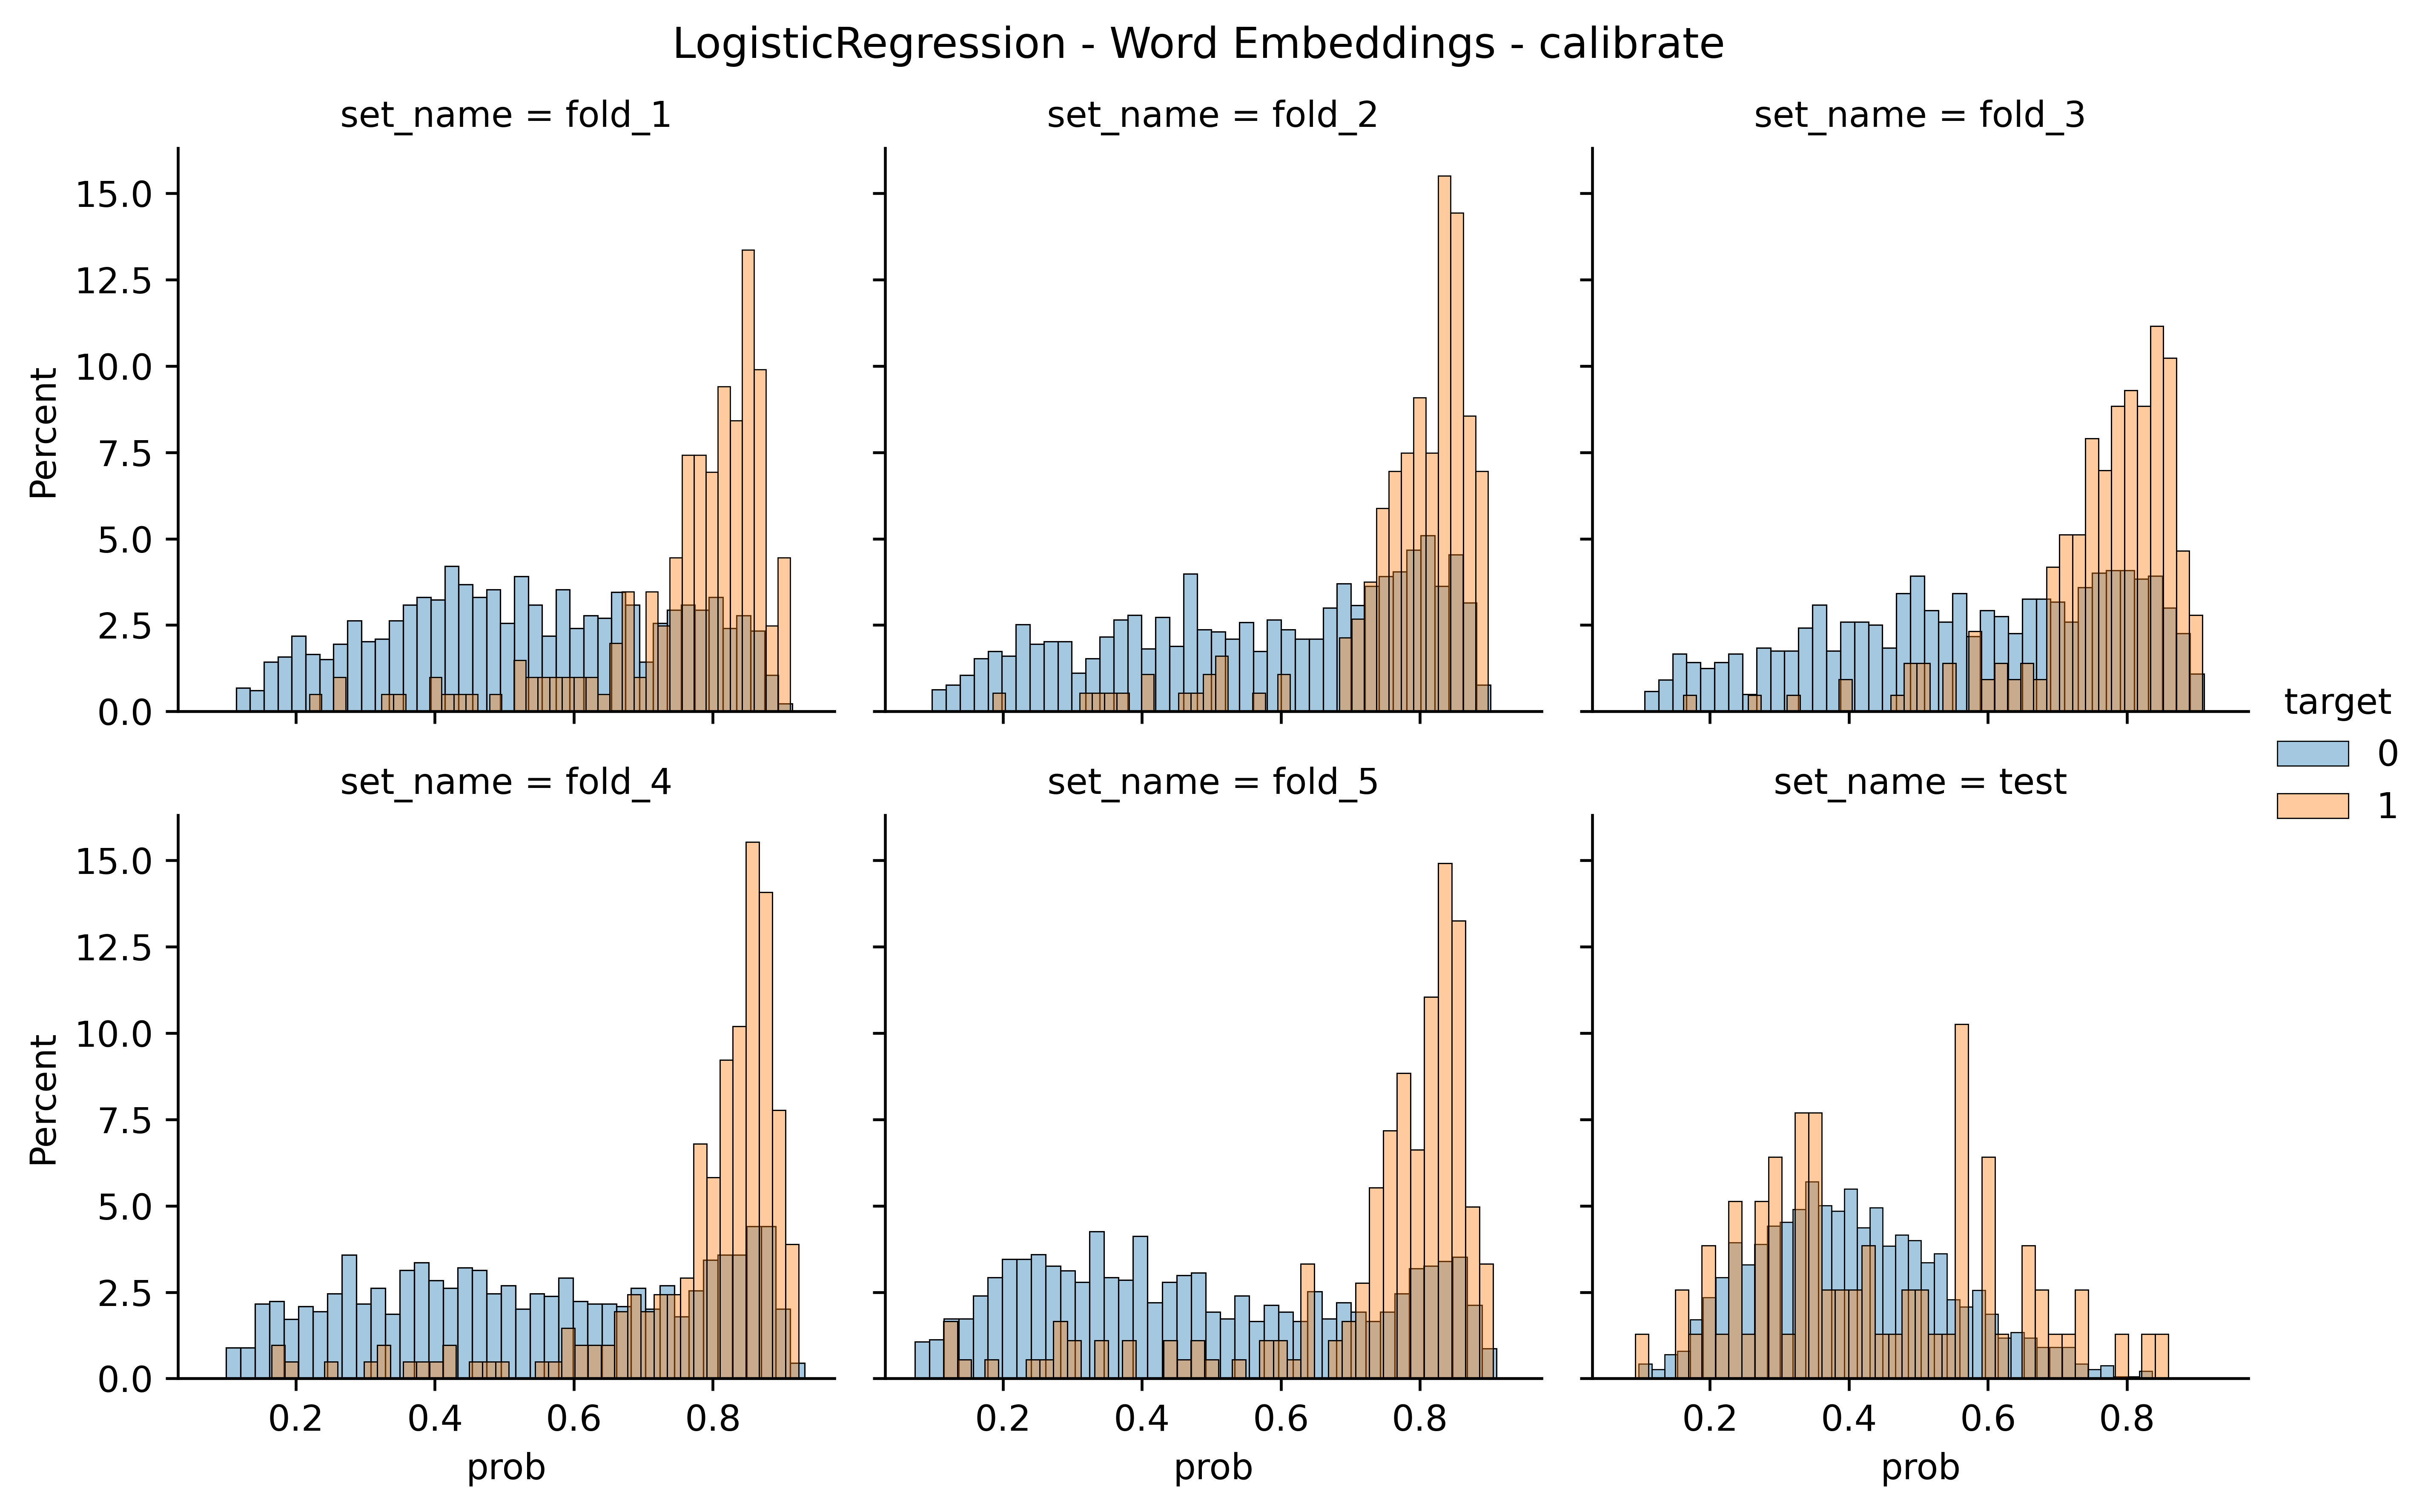
\includegraphics[width=\linewidth]{figures/results/word_embeddings/lgr/calibrate/calibrate__distplot.png}
    \end{subfigure}
    \hfill
    \centering
    \begin{subfigure}[b]{0.83\textwidth}
        \centering
        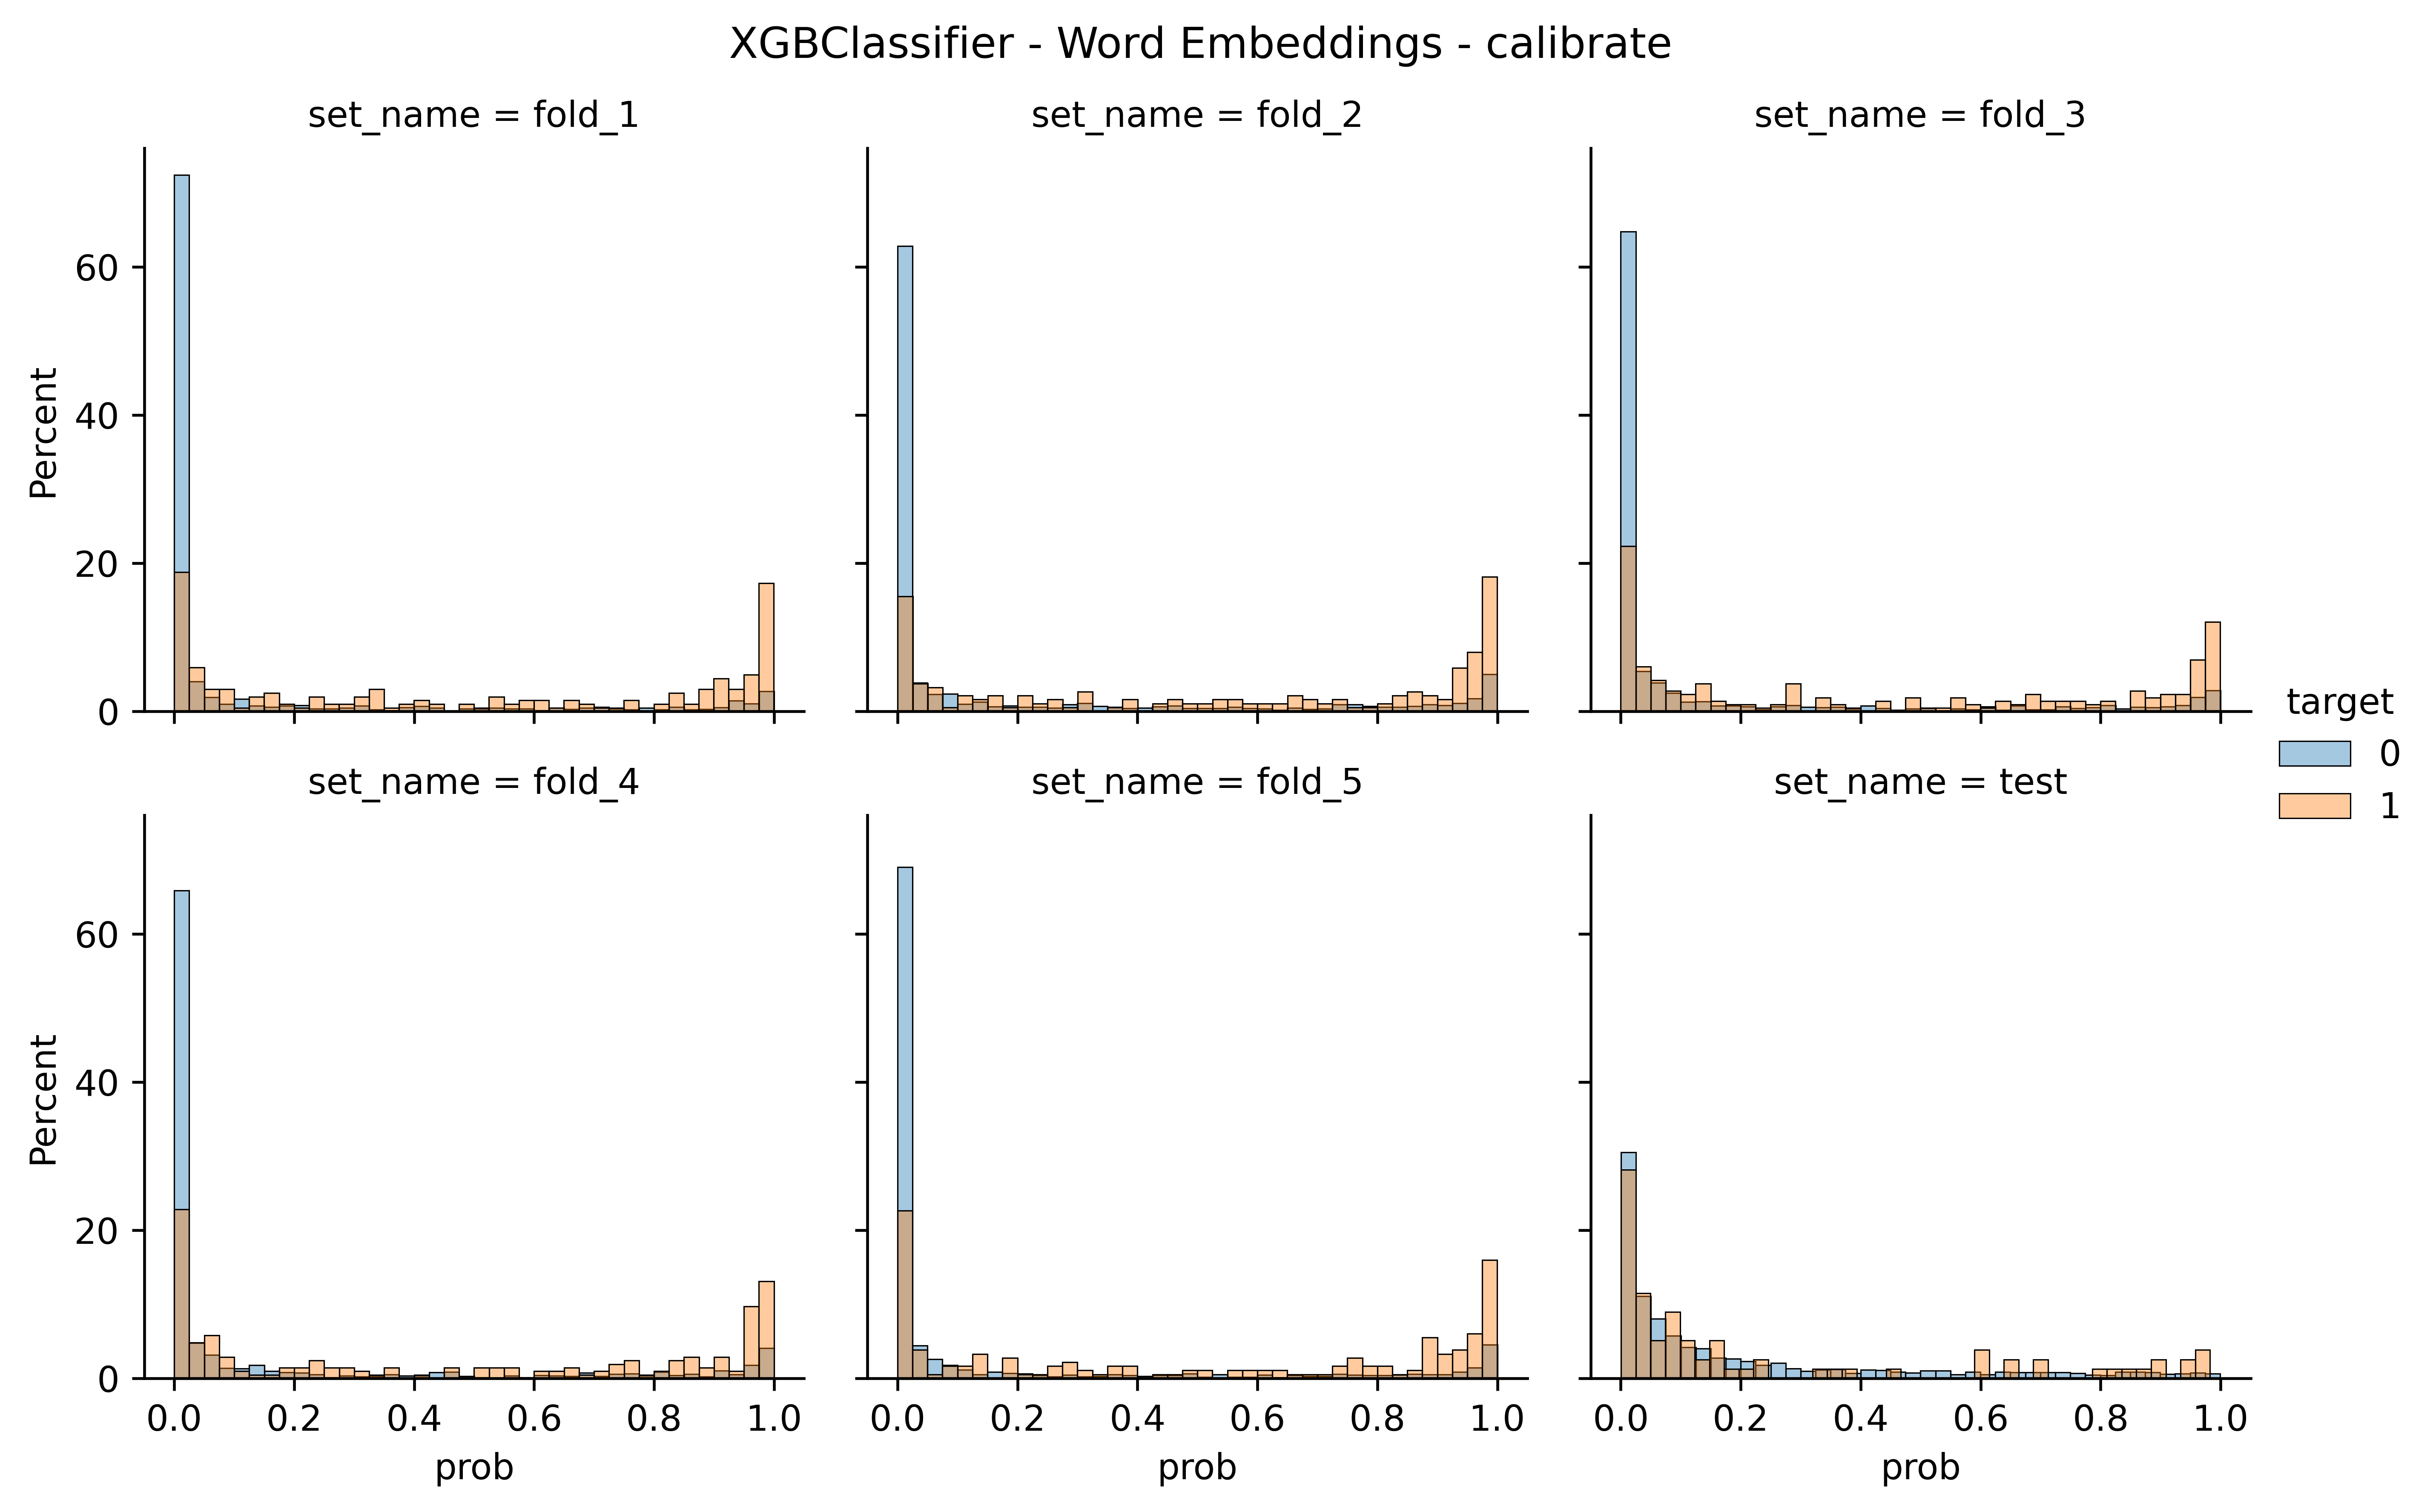
\includegraphics[width=\linewidth]{figures/results/word_embeddings/xgboost/calibrate/calibrate__distplot.png}
    \end{subfigure}
    \hfill
    \centering
    \begin{subfigure}[b]{0.83\textwidth}
        \centering
        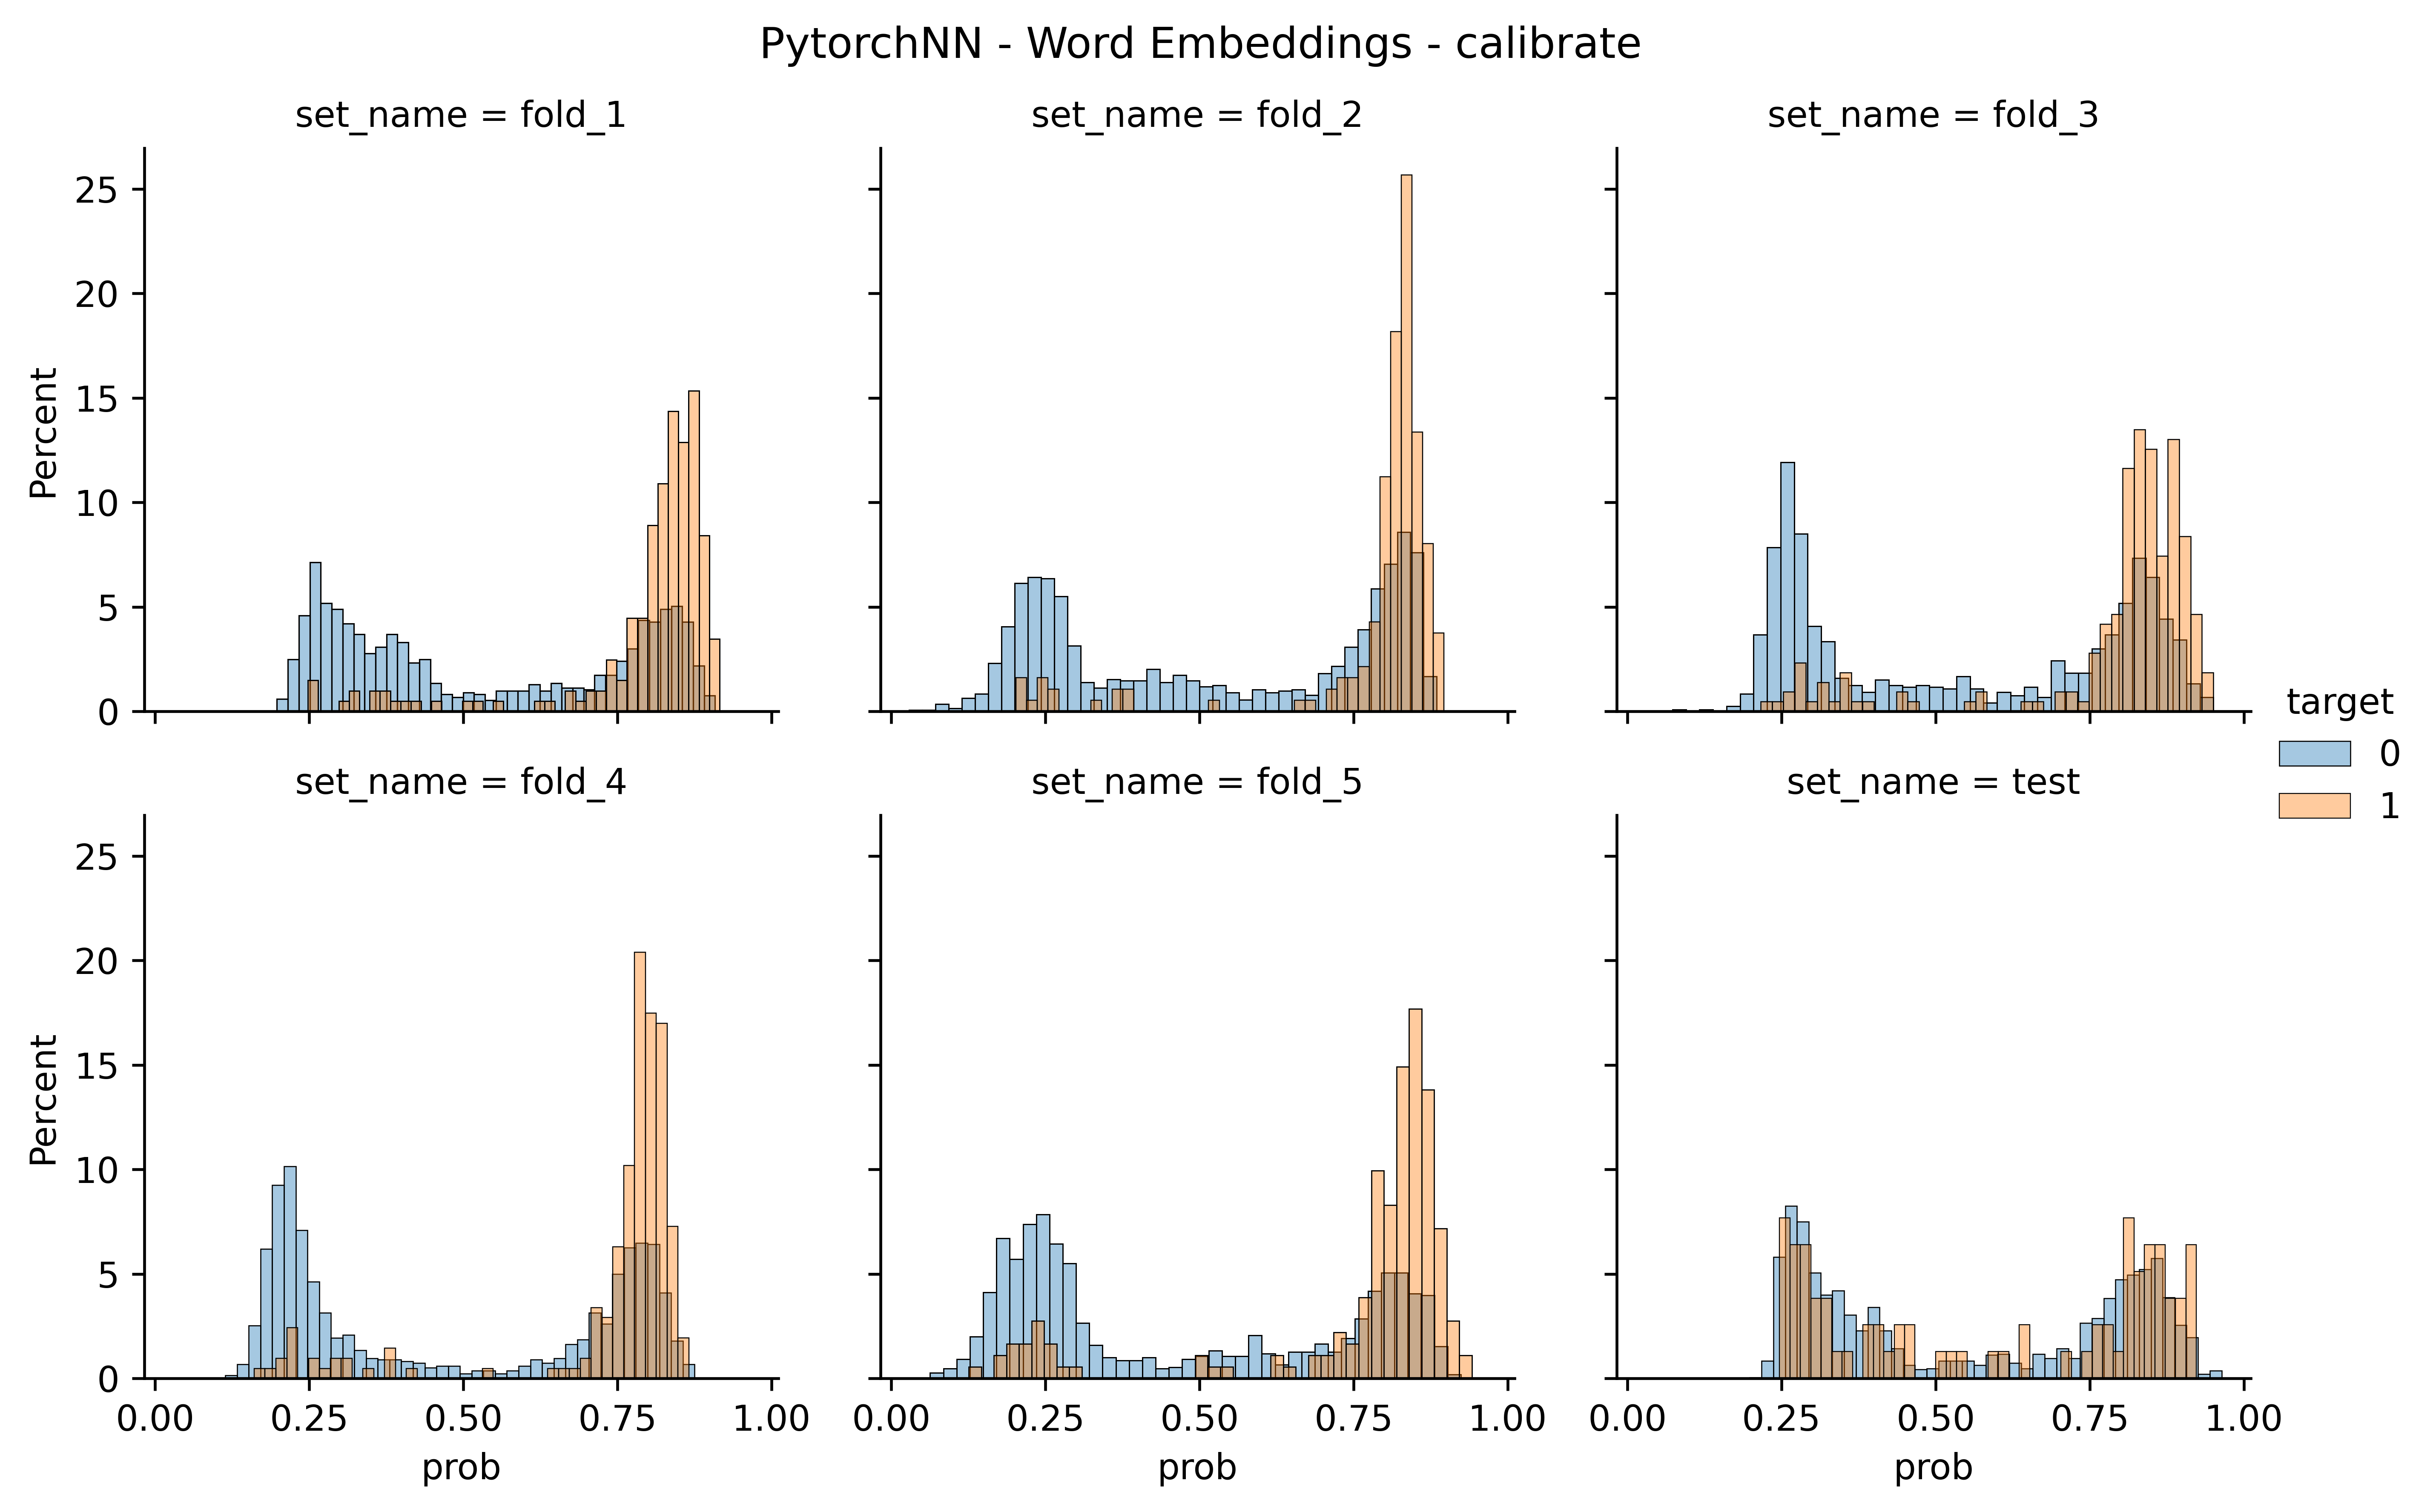
\includegraphics[width=\linewidth]{figures/results/word_embeddings/nn/calibrate/calibrate__distplot.png}
    \end{subfigure}
    \caption{Word embeddings calibrate}
\end{figure}

\begin{figure}
    \centering
    \begin{subfigure}[b]{0.83\textwidth}
    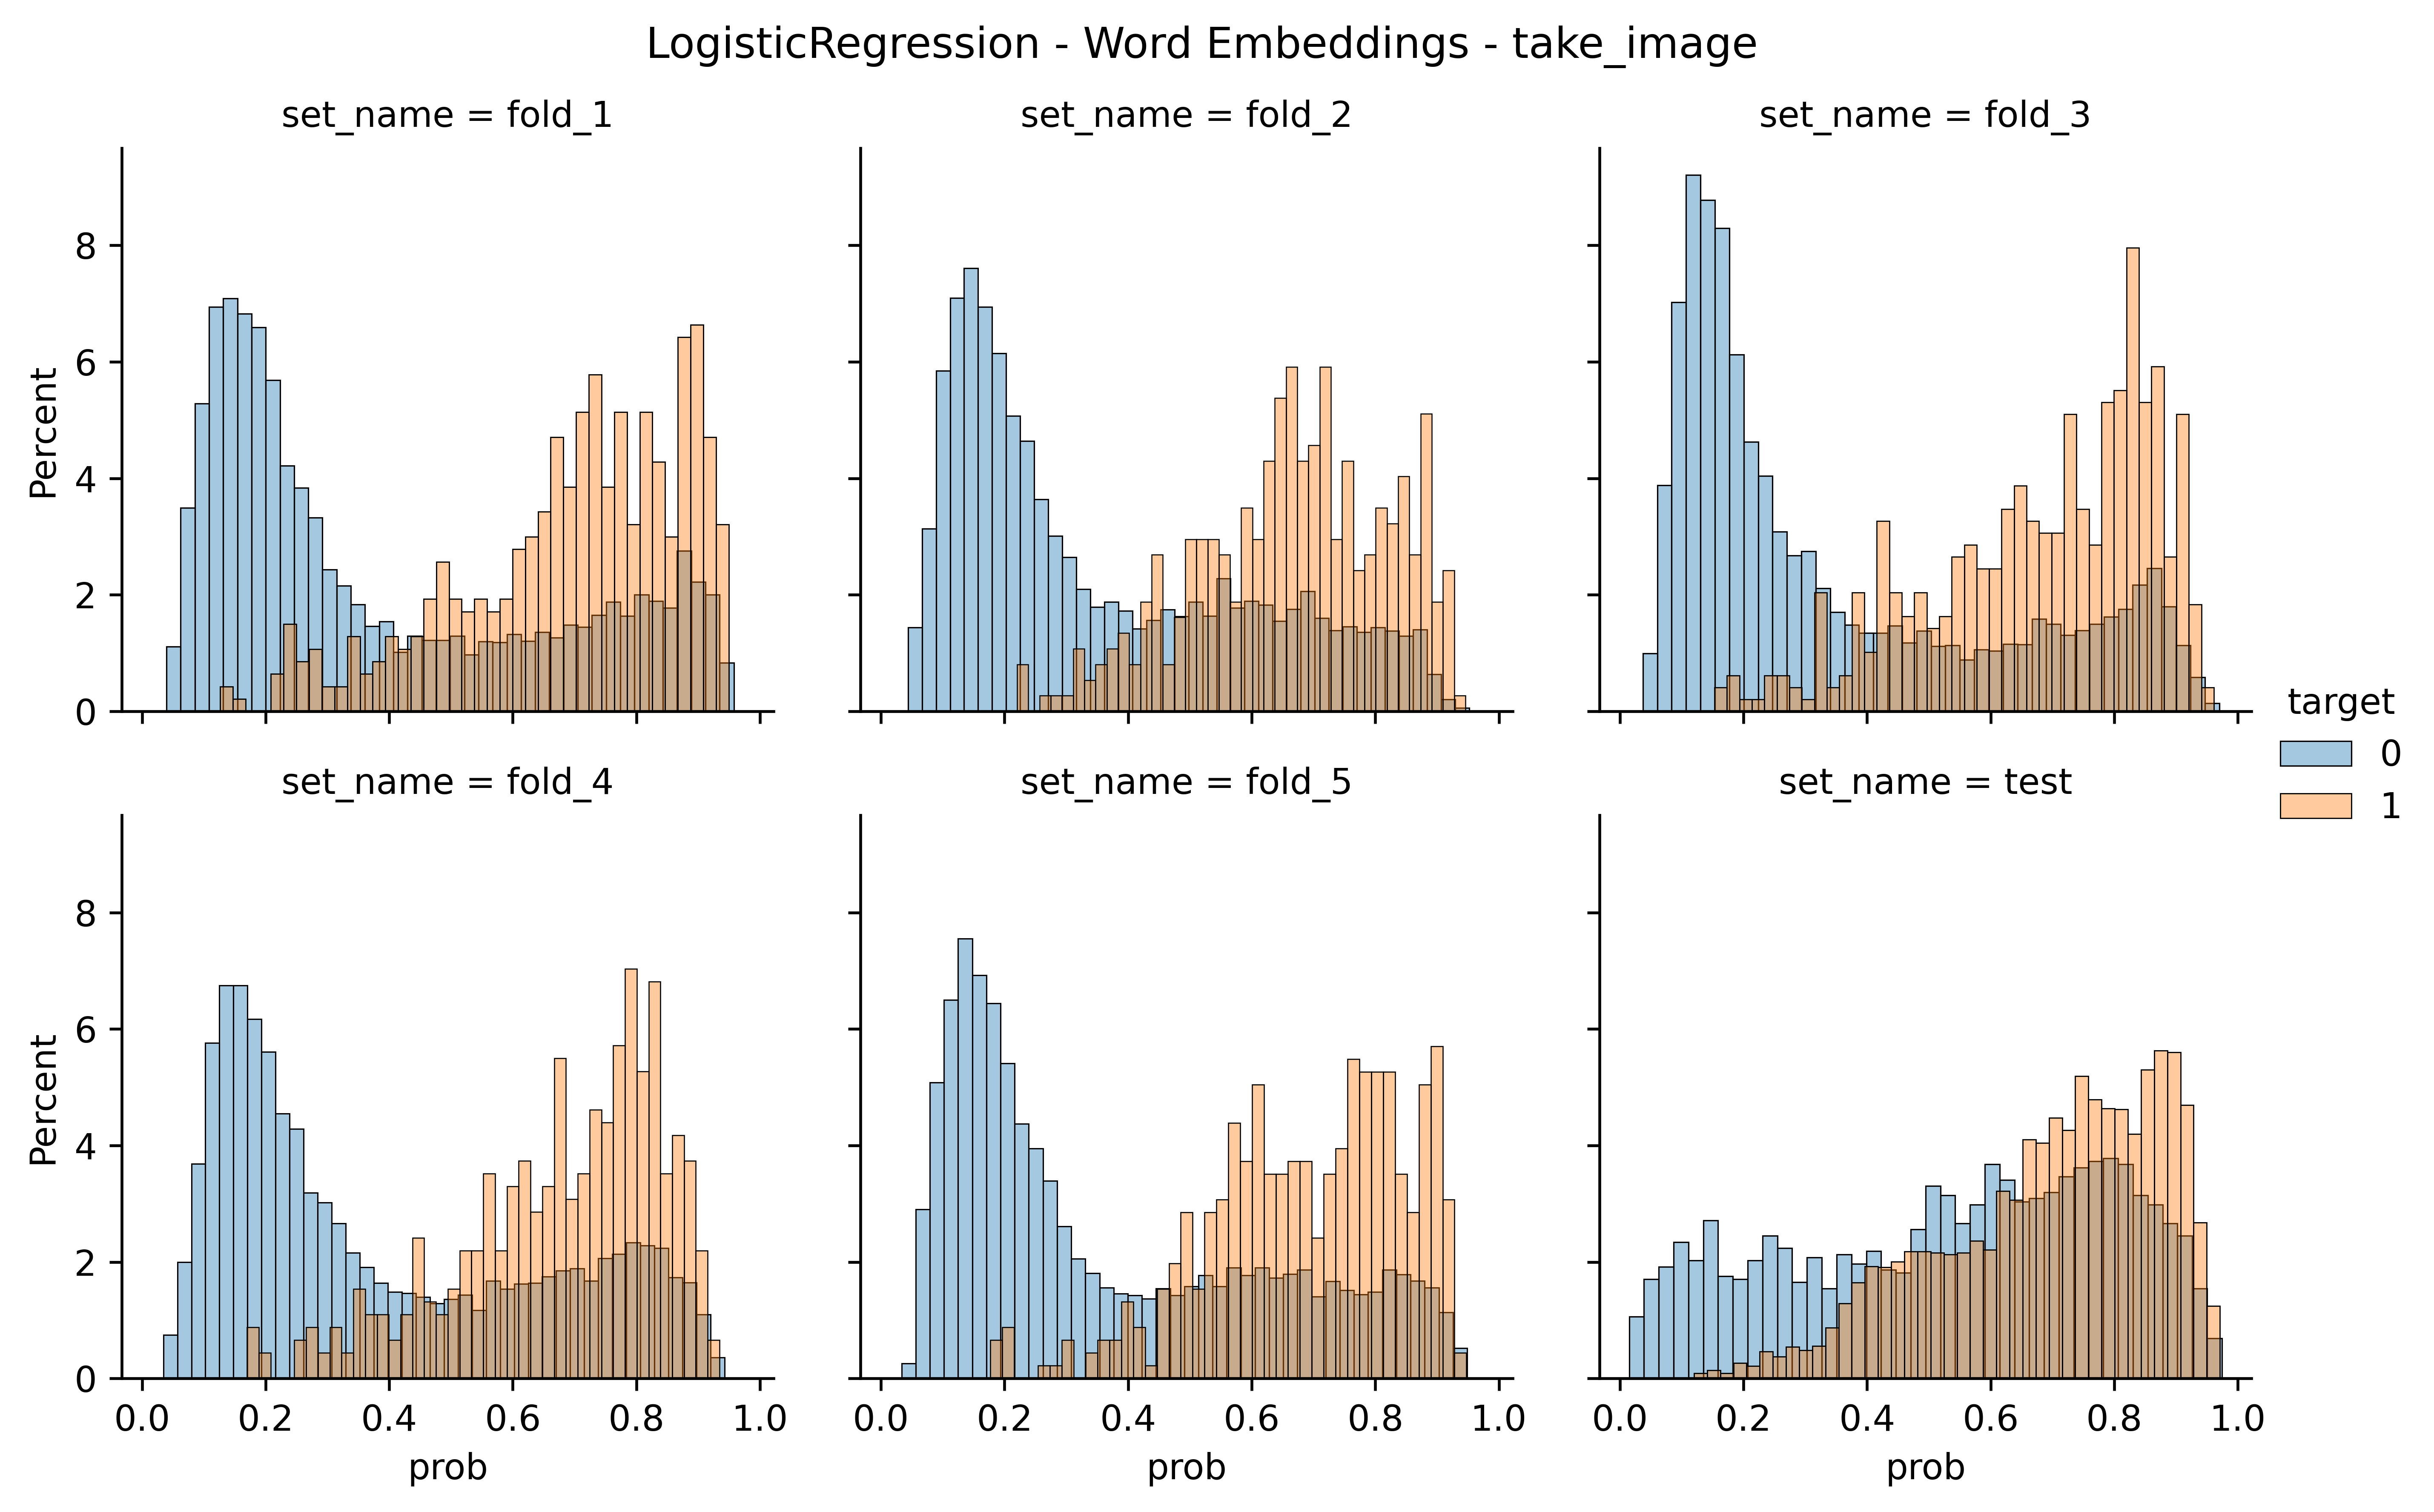
\includegraphics[width=\linewidth]{figures/results/word_embeddings/lgr/take_image/lgr__distplot.png}
    \end{subfigure}
    \hfill
    \centering
    \begin{subfigure}[b]{0.83\textwidth}
        \centering
        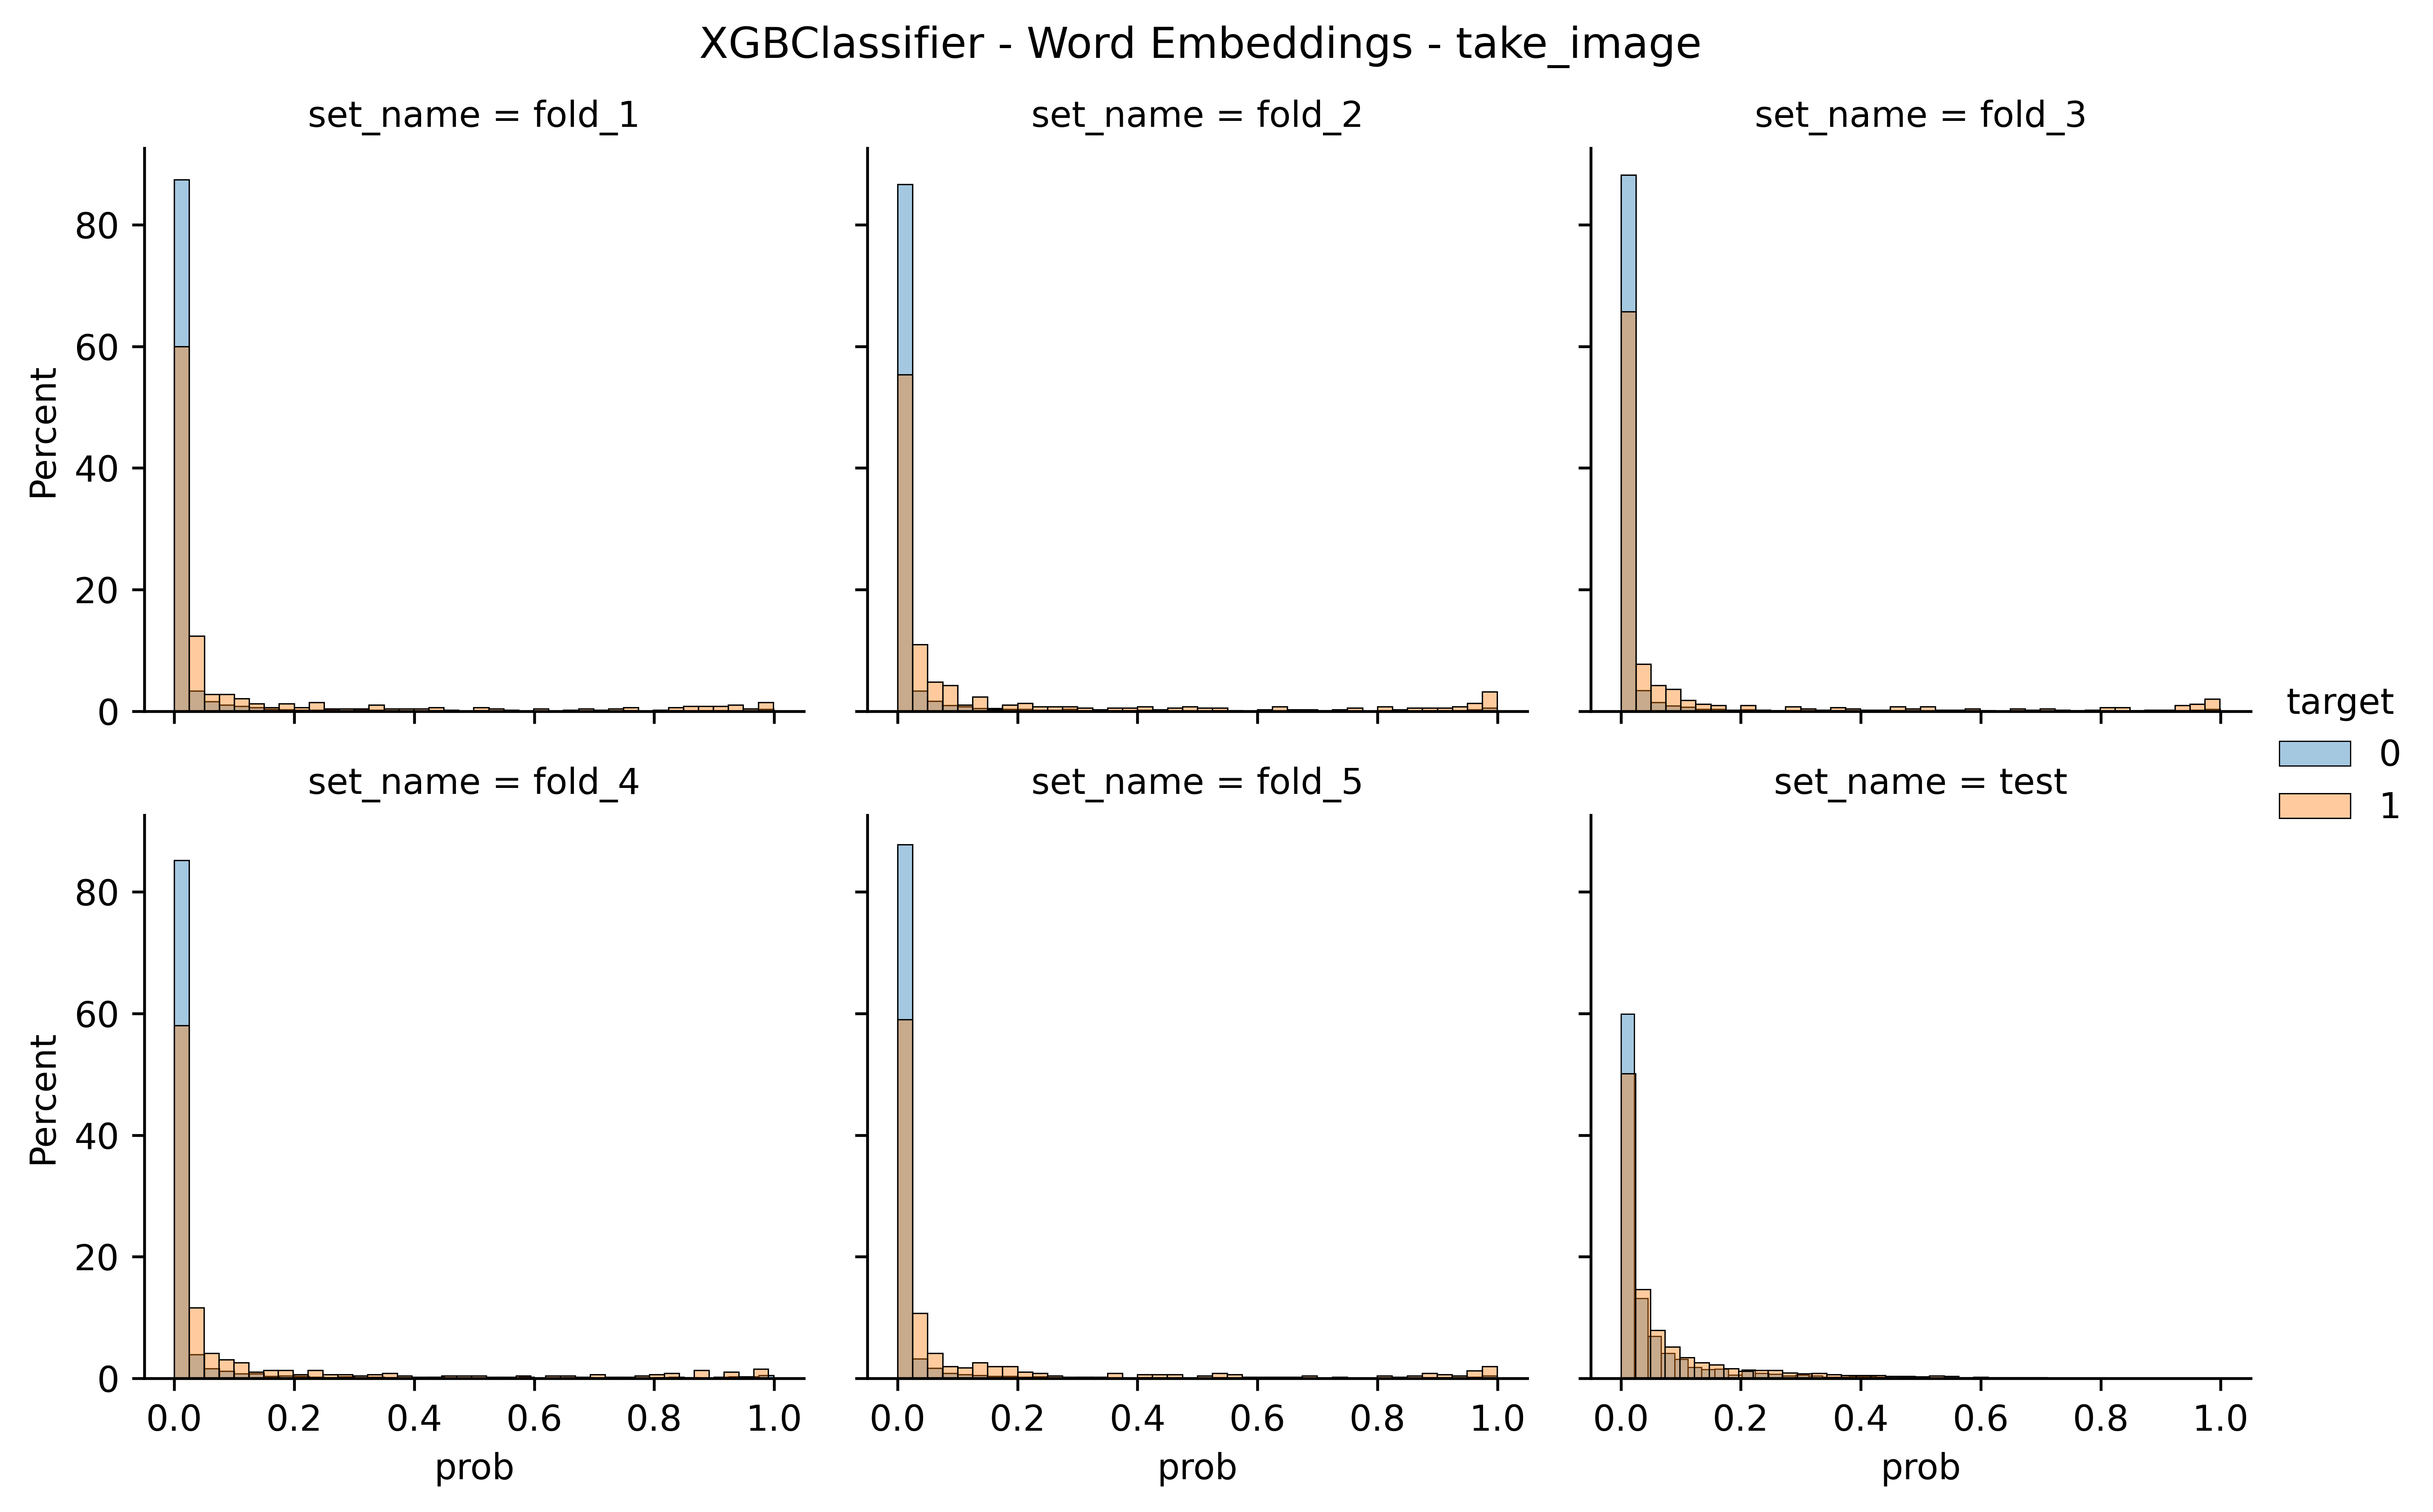
\includegraphics[width=\linewidth]{figures/results/word_embeddings/xgboost/take_image/take_image__distplot.png}
    \end{subfigure}
    \hfill
    \centering
    \begin{subfigure}[b]{0.83\textwidth}
        \centering
        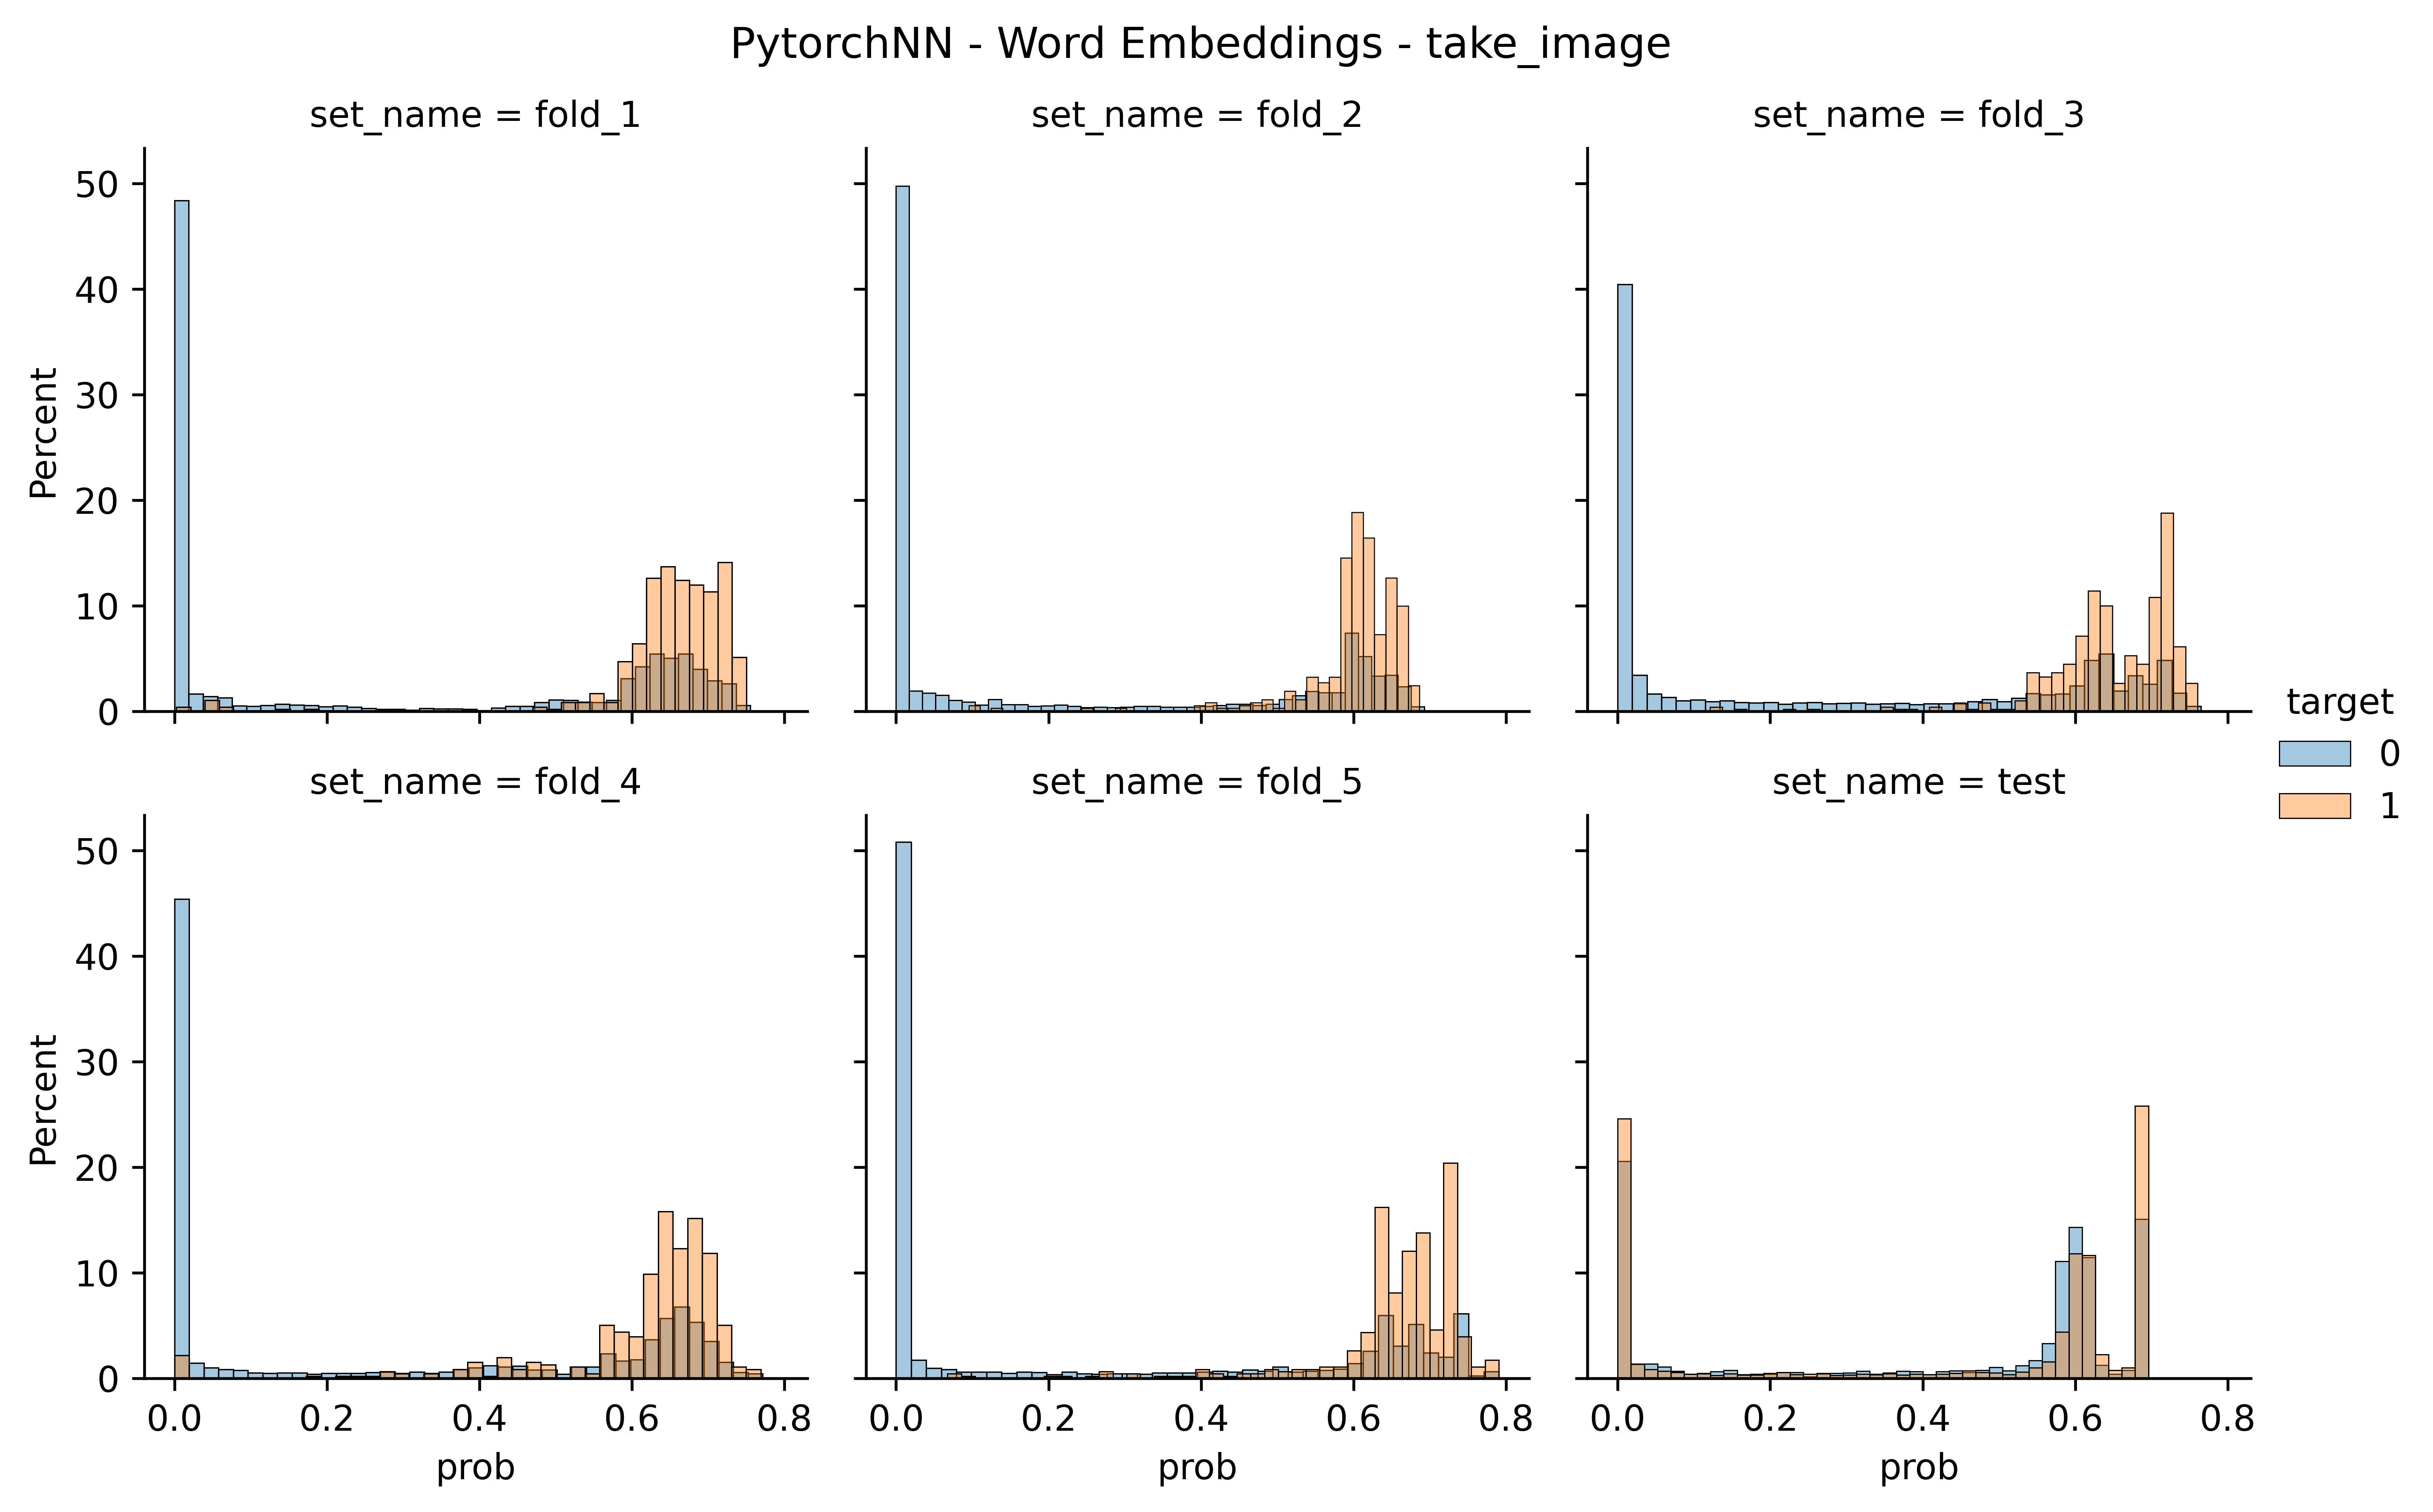
\includegraphics[width=\linewidth]{figures/results/word_embeddings/nn/take_image/take_image__distplot (1).png}
    \end{subfigure}
    \caption{Word embeddings take\_image}
\end{figure}

\begin{figure}
    \centering
    \begin{subfigure}[b]{0.83\textwidth}
    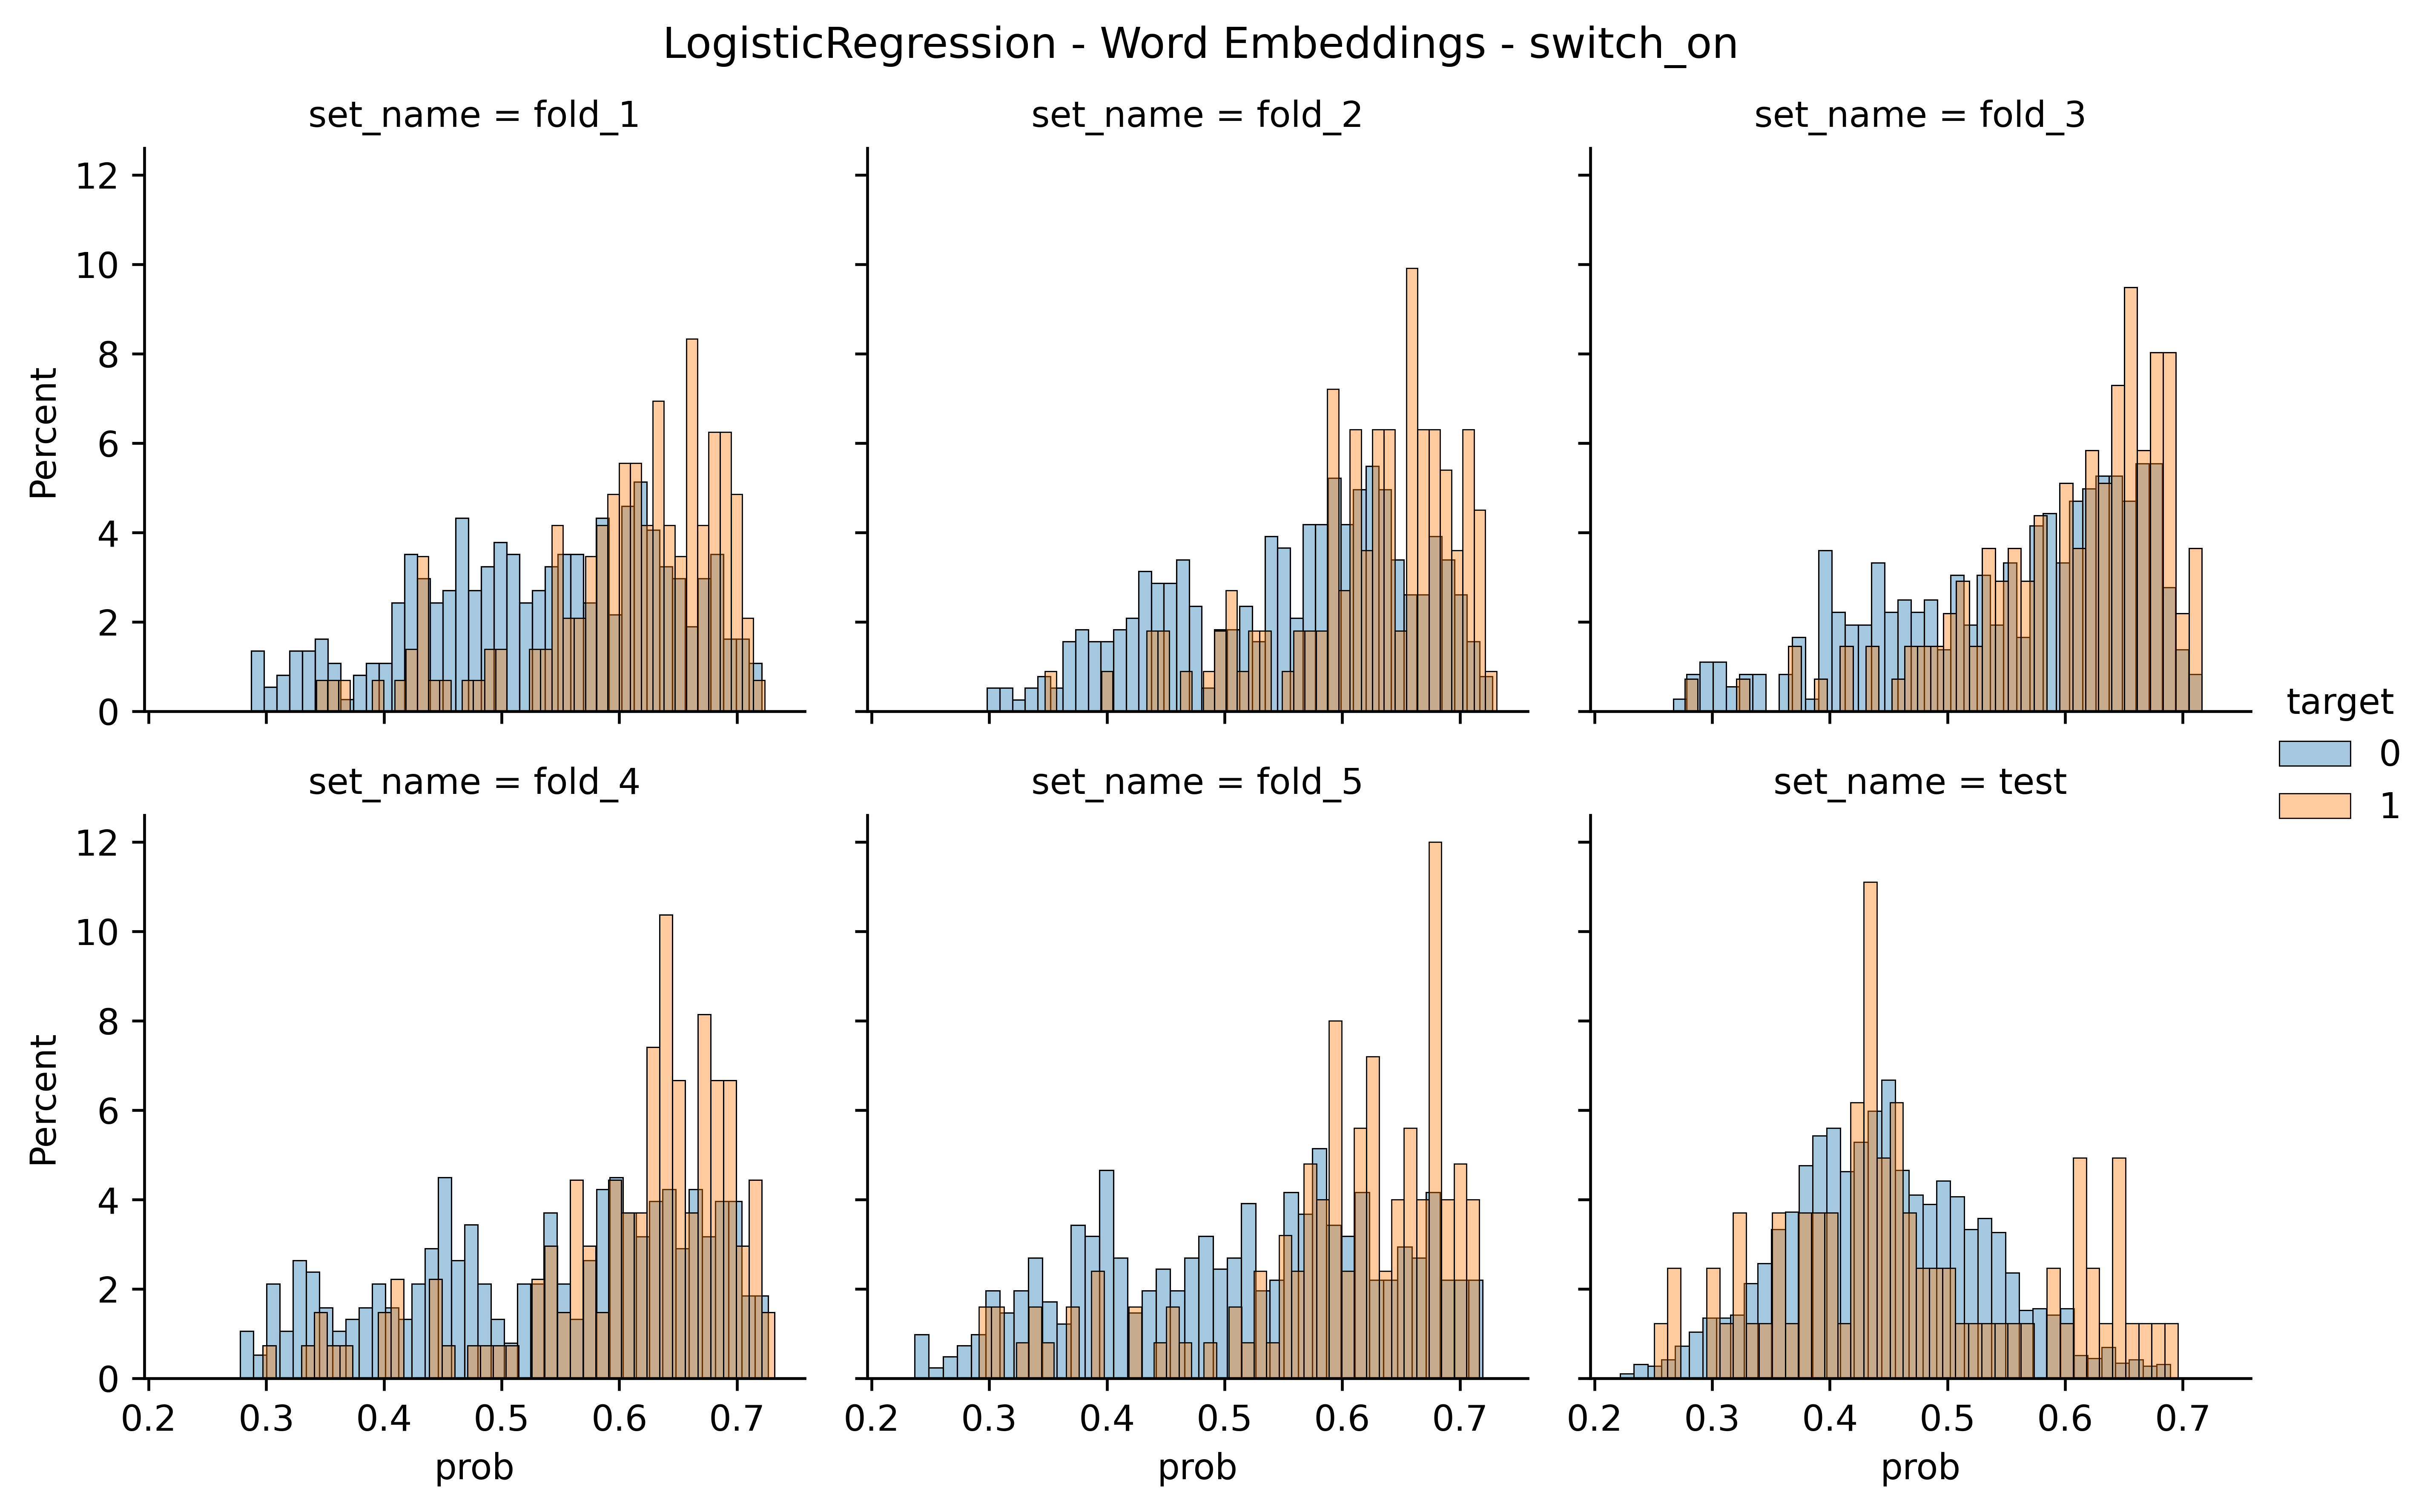
\includegraphics[width=\linewidth]{figures/results/word_embeddings/lgr/switch_on/switch_on__distplot.png}
    \end{subfigure}
    \hfill
    \centering
    \begin{subfigure}[b]{0.83\textwidth}
        \centering
        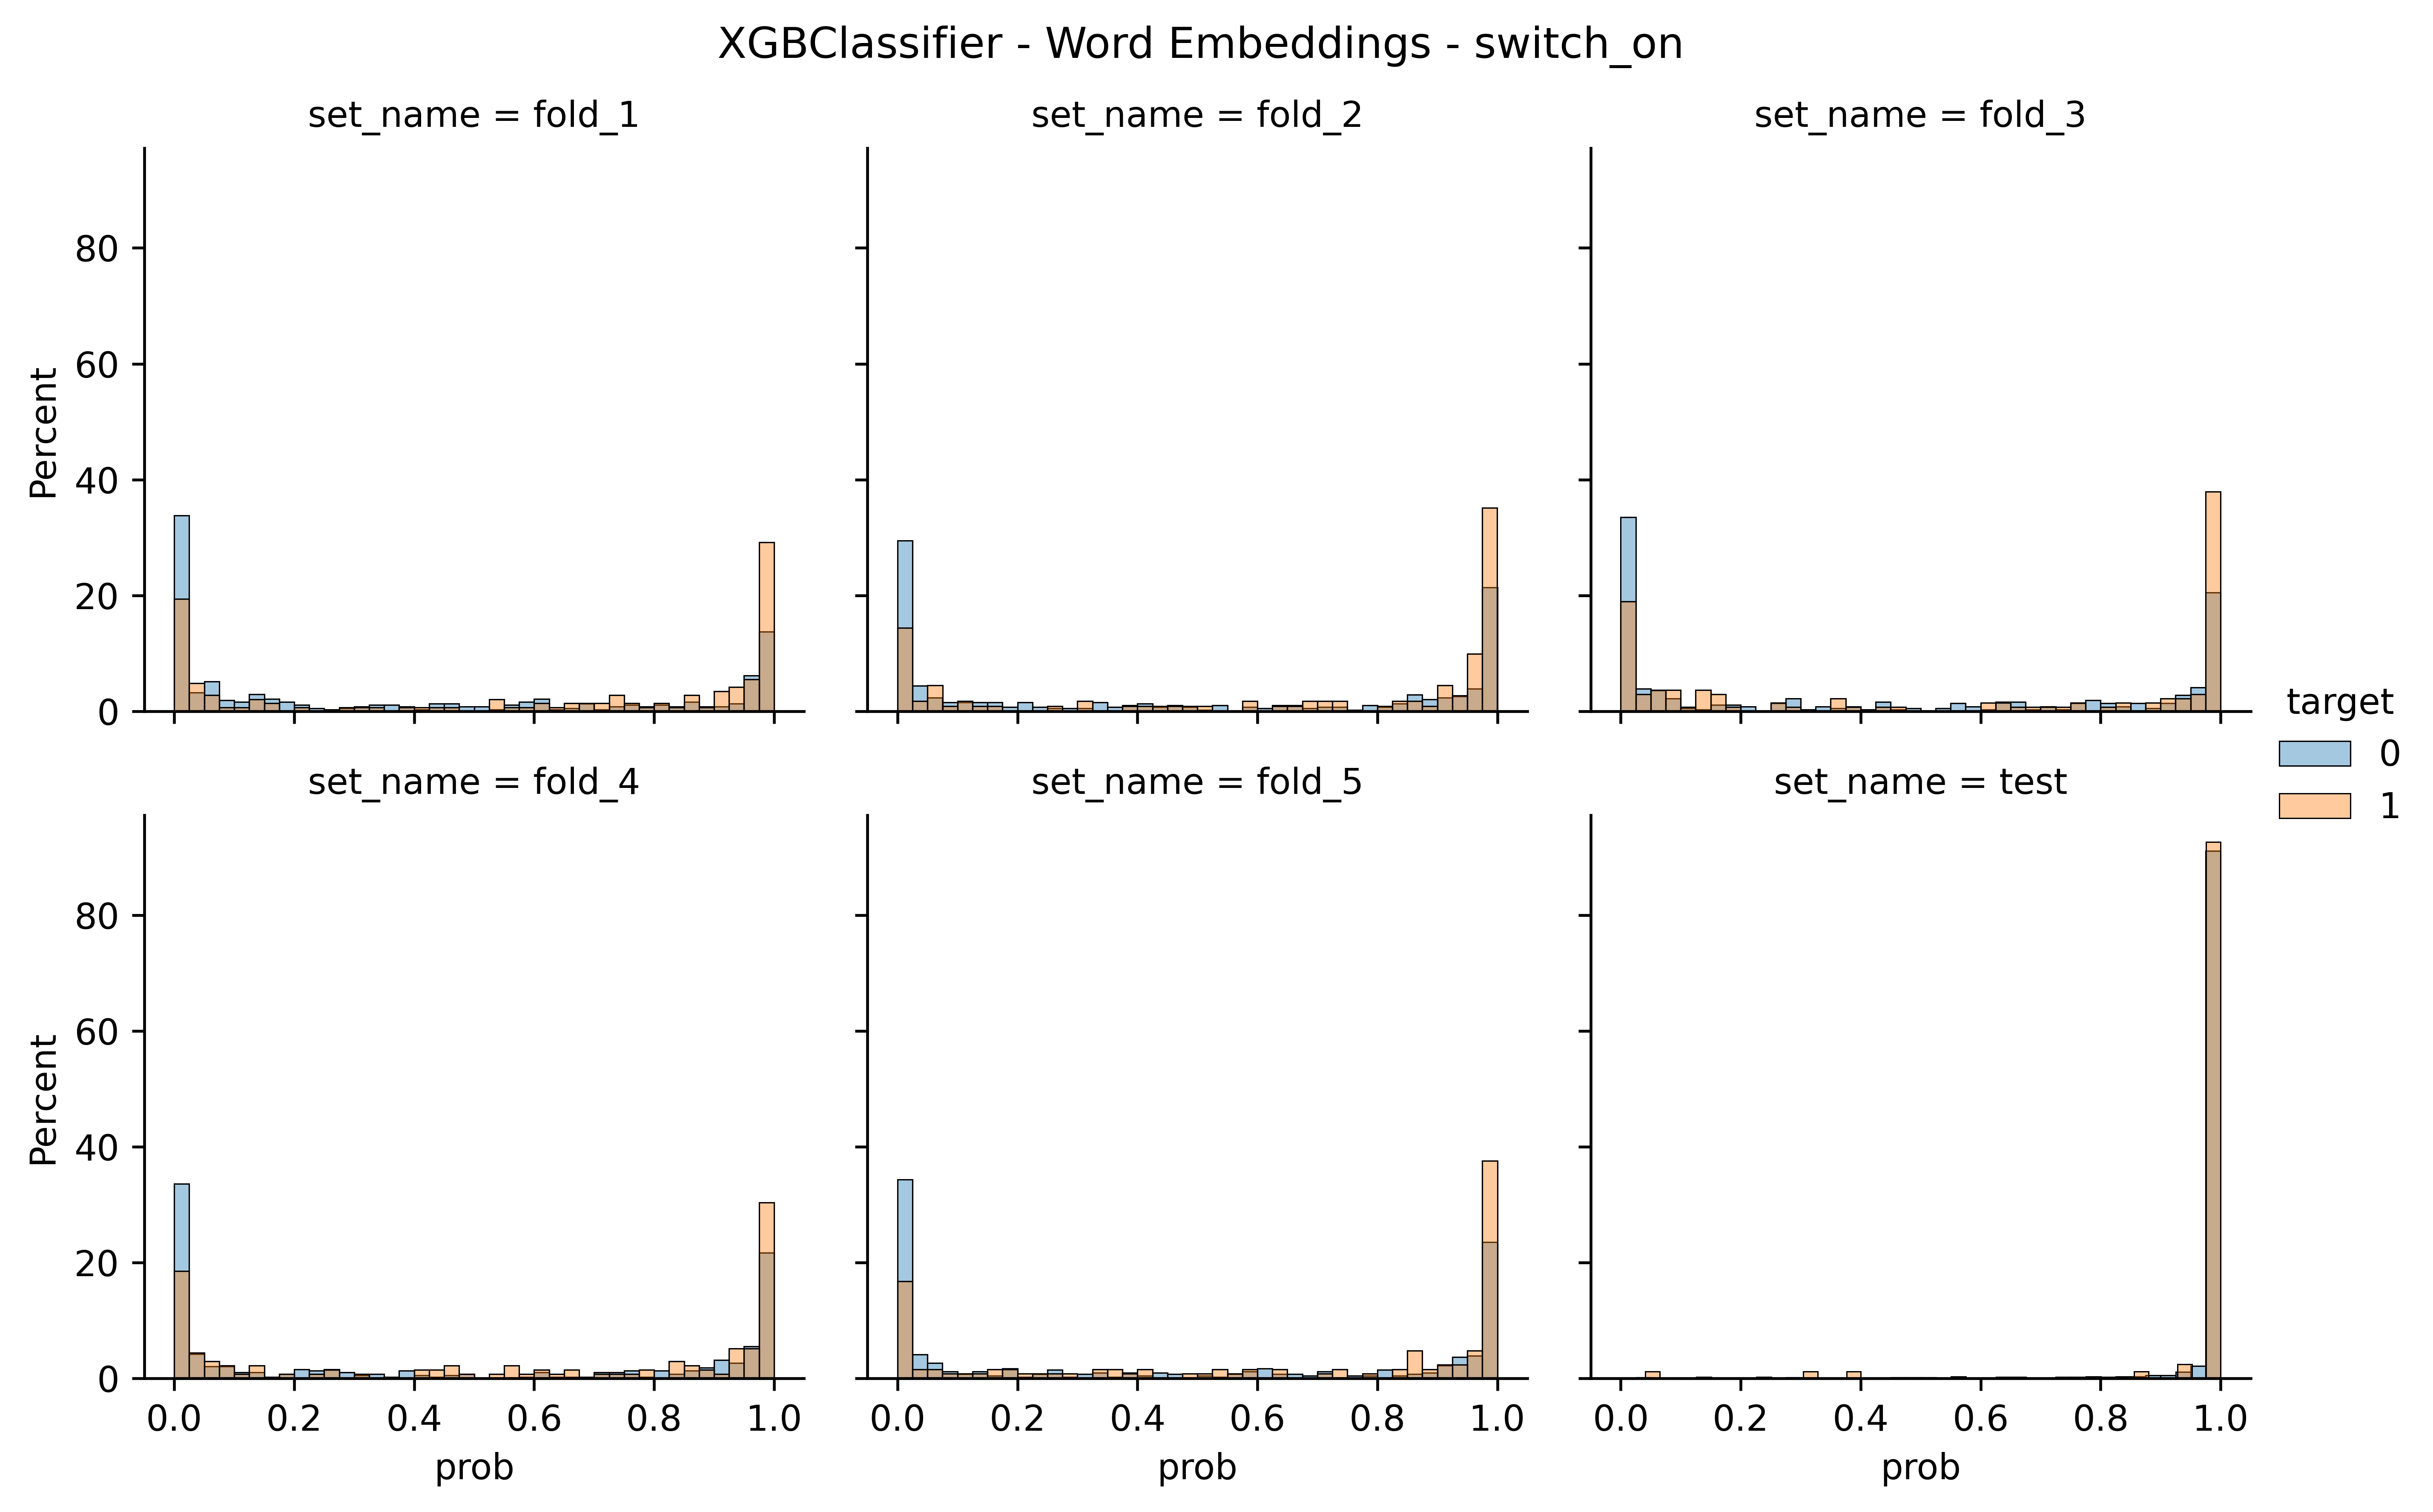
\includegraphics[width=\linewidth]{figures/results/word_embeddings/xgboost/switch_on/xgb__distplot.png}
    \end{subfigure}
    \hfill
    \centering
    \begin{subfigure}[b]{0.83\textwidth}
        \centering
        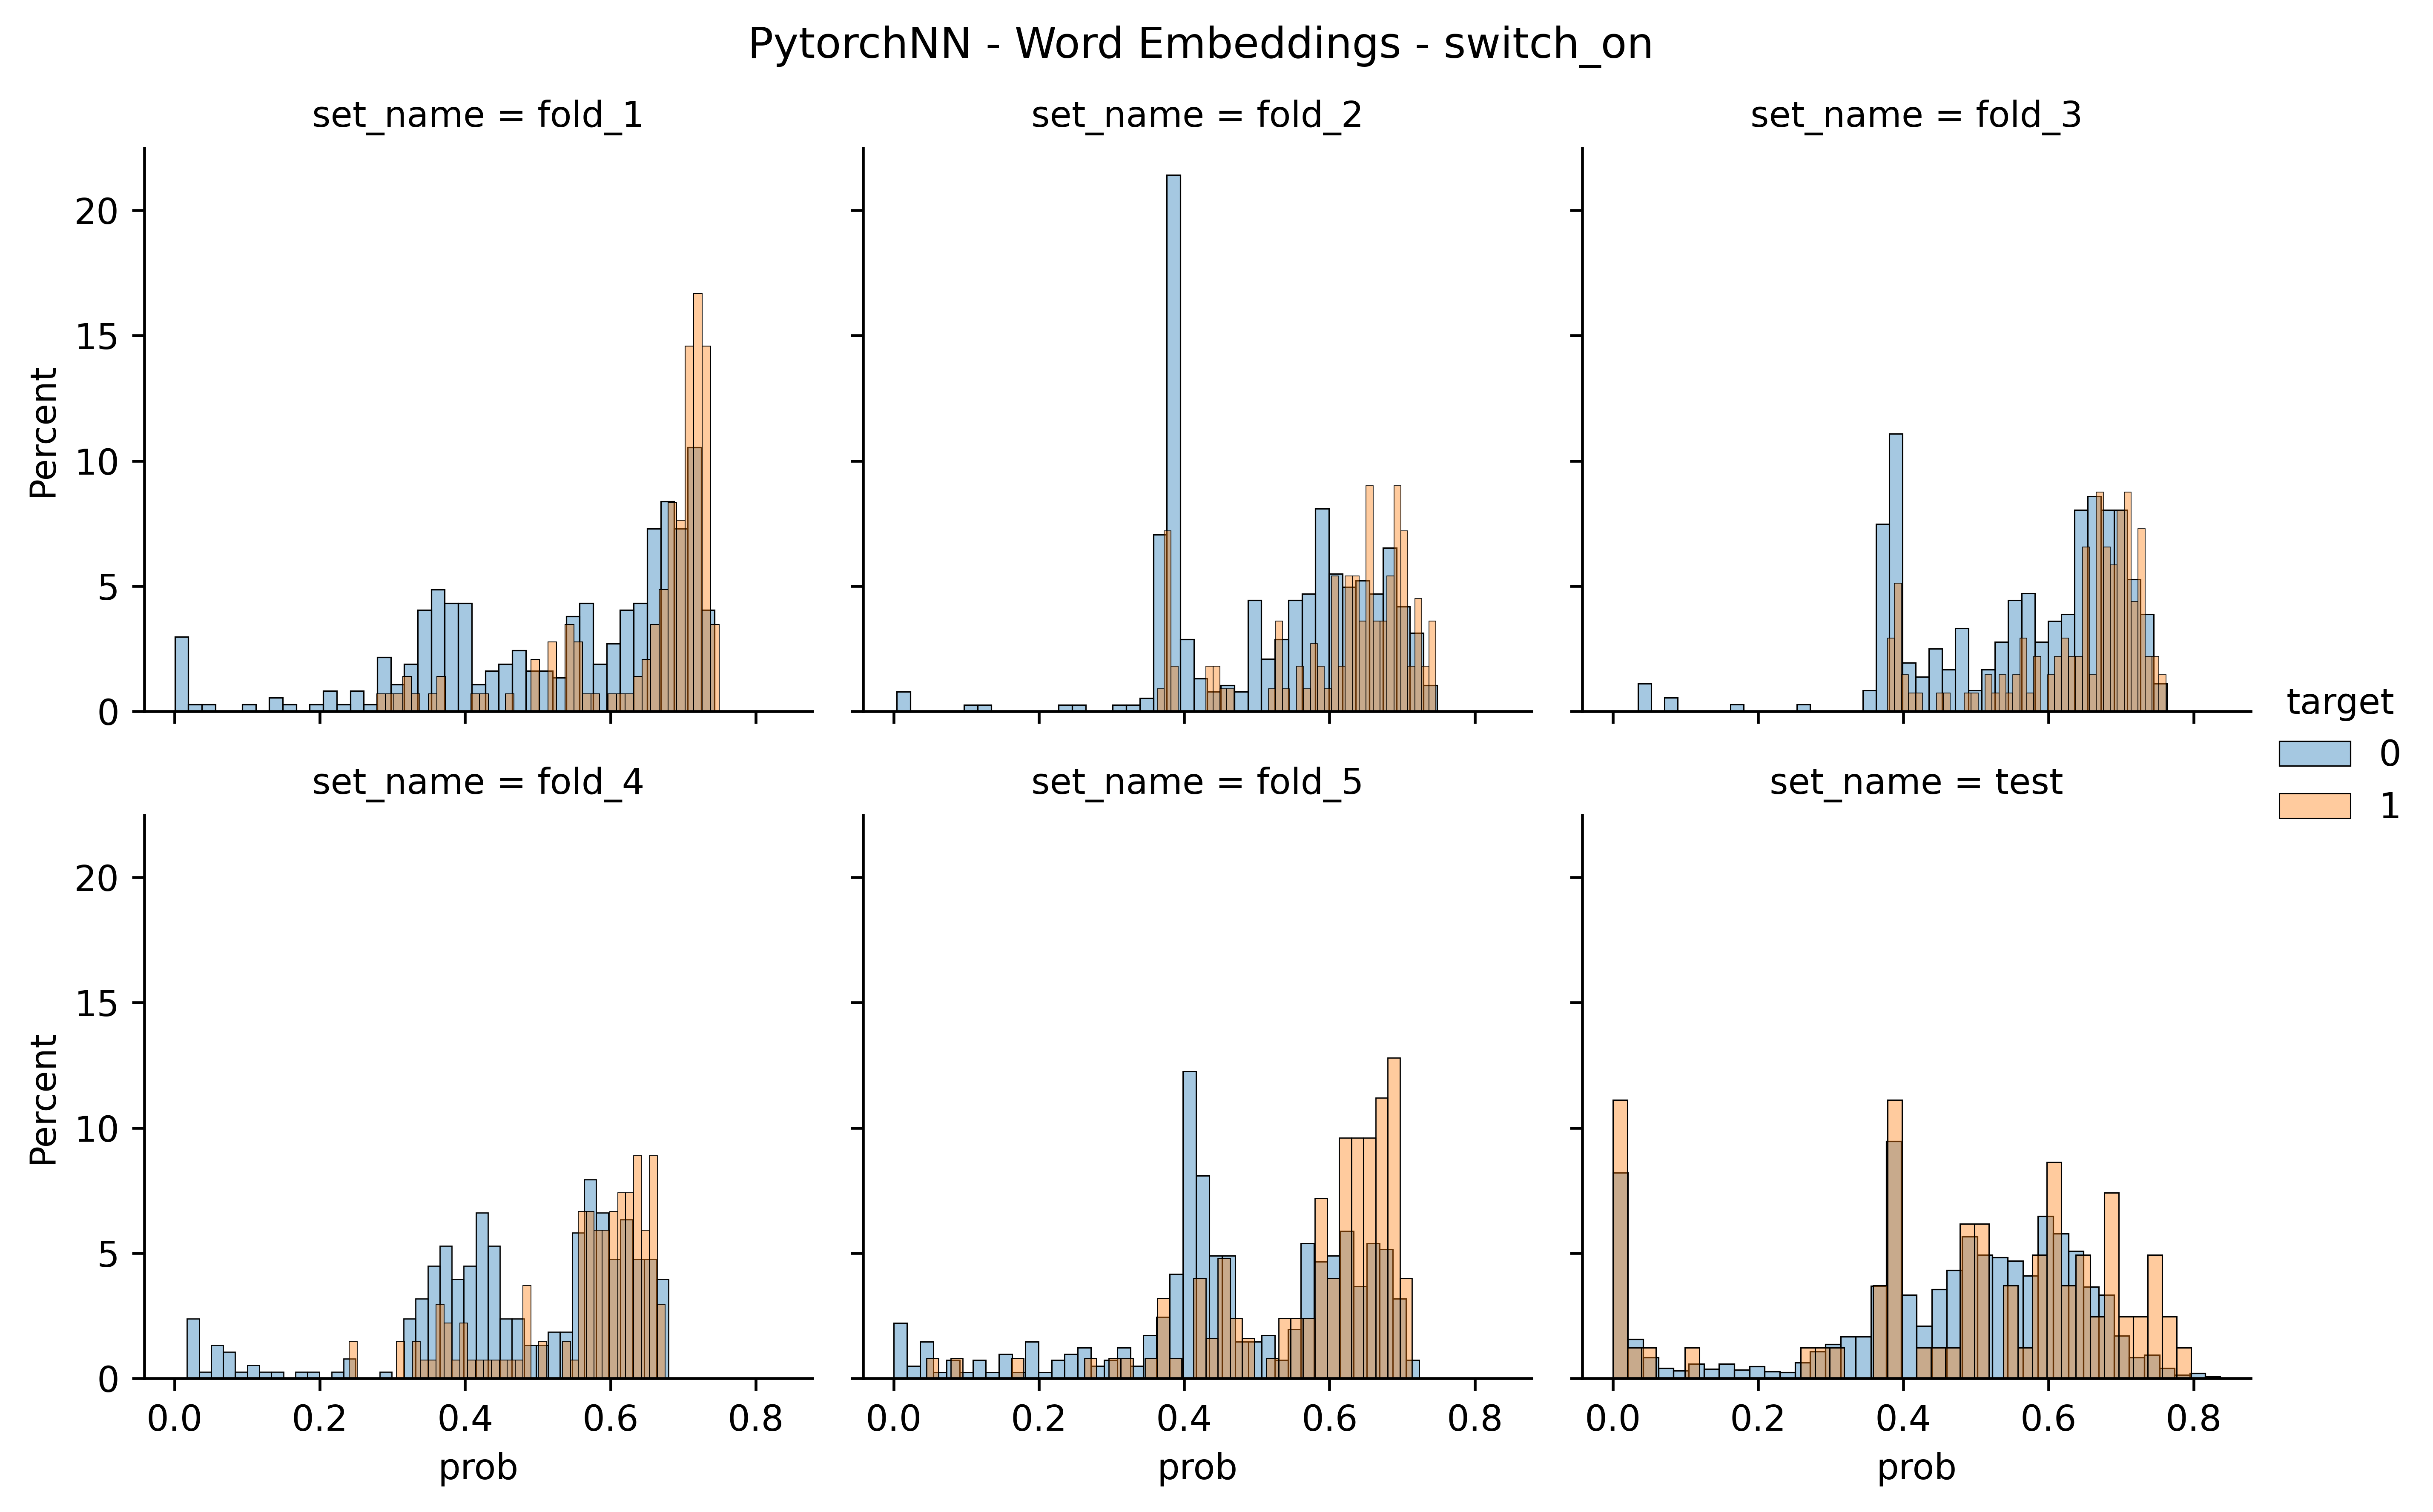
\includegraphics[width=\linewidth]{figures/results/word_embeddings/nn/switch_on/switch_on__distplot (1).png}
    \end{subfigure}
    \caption{Word embeddings switch\_on}
\end{figure}


\begin{figure}
    \begin{subfigure}[b]{\textwidth}
        \centering
        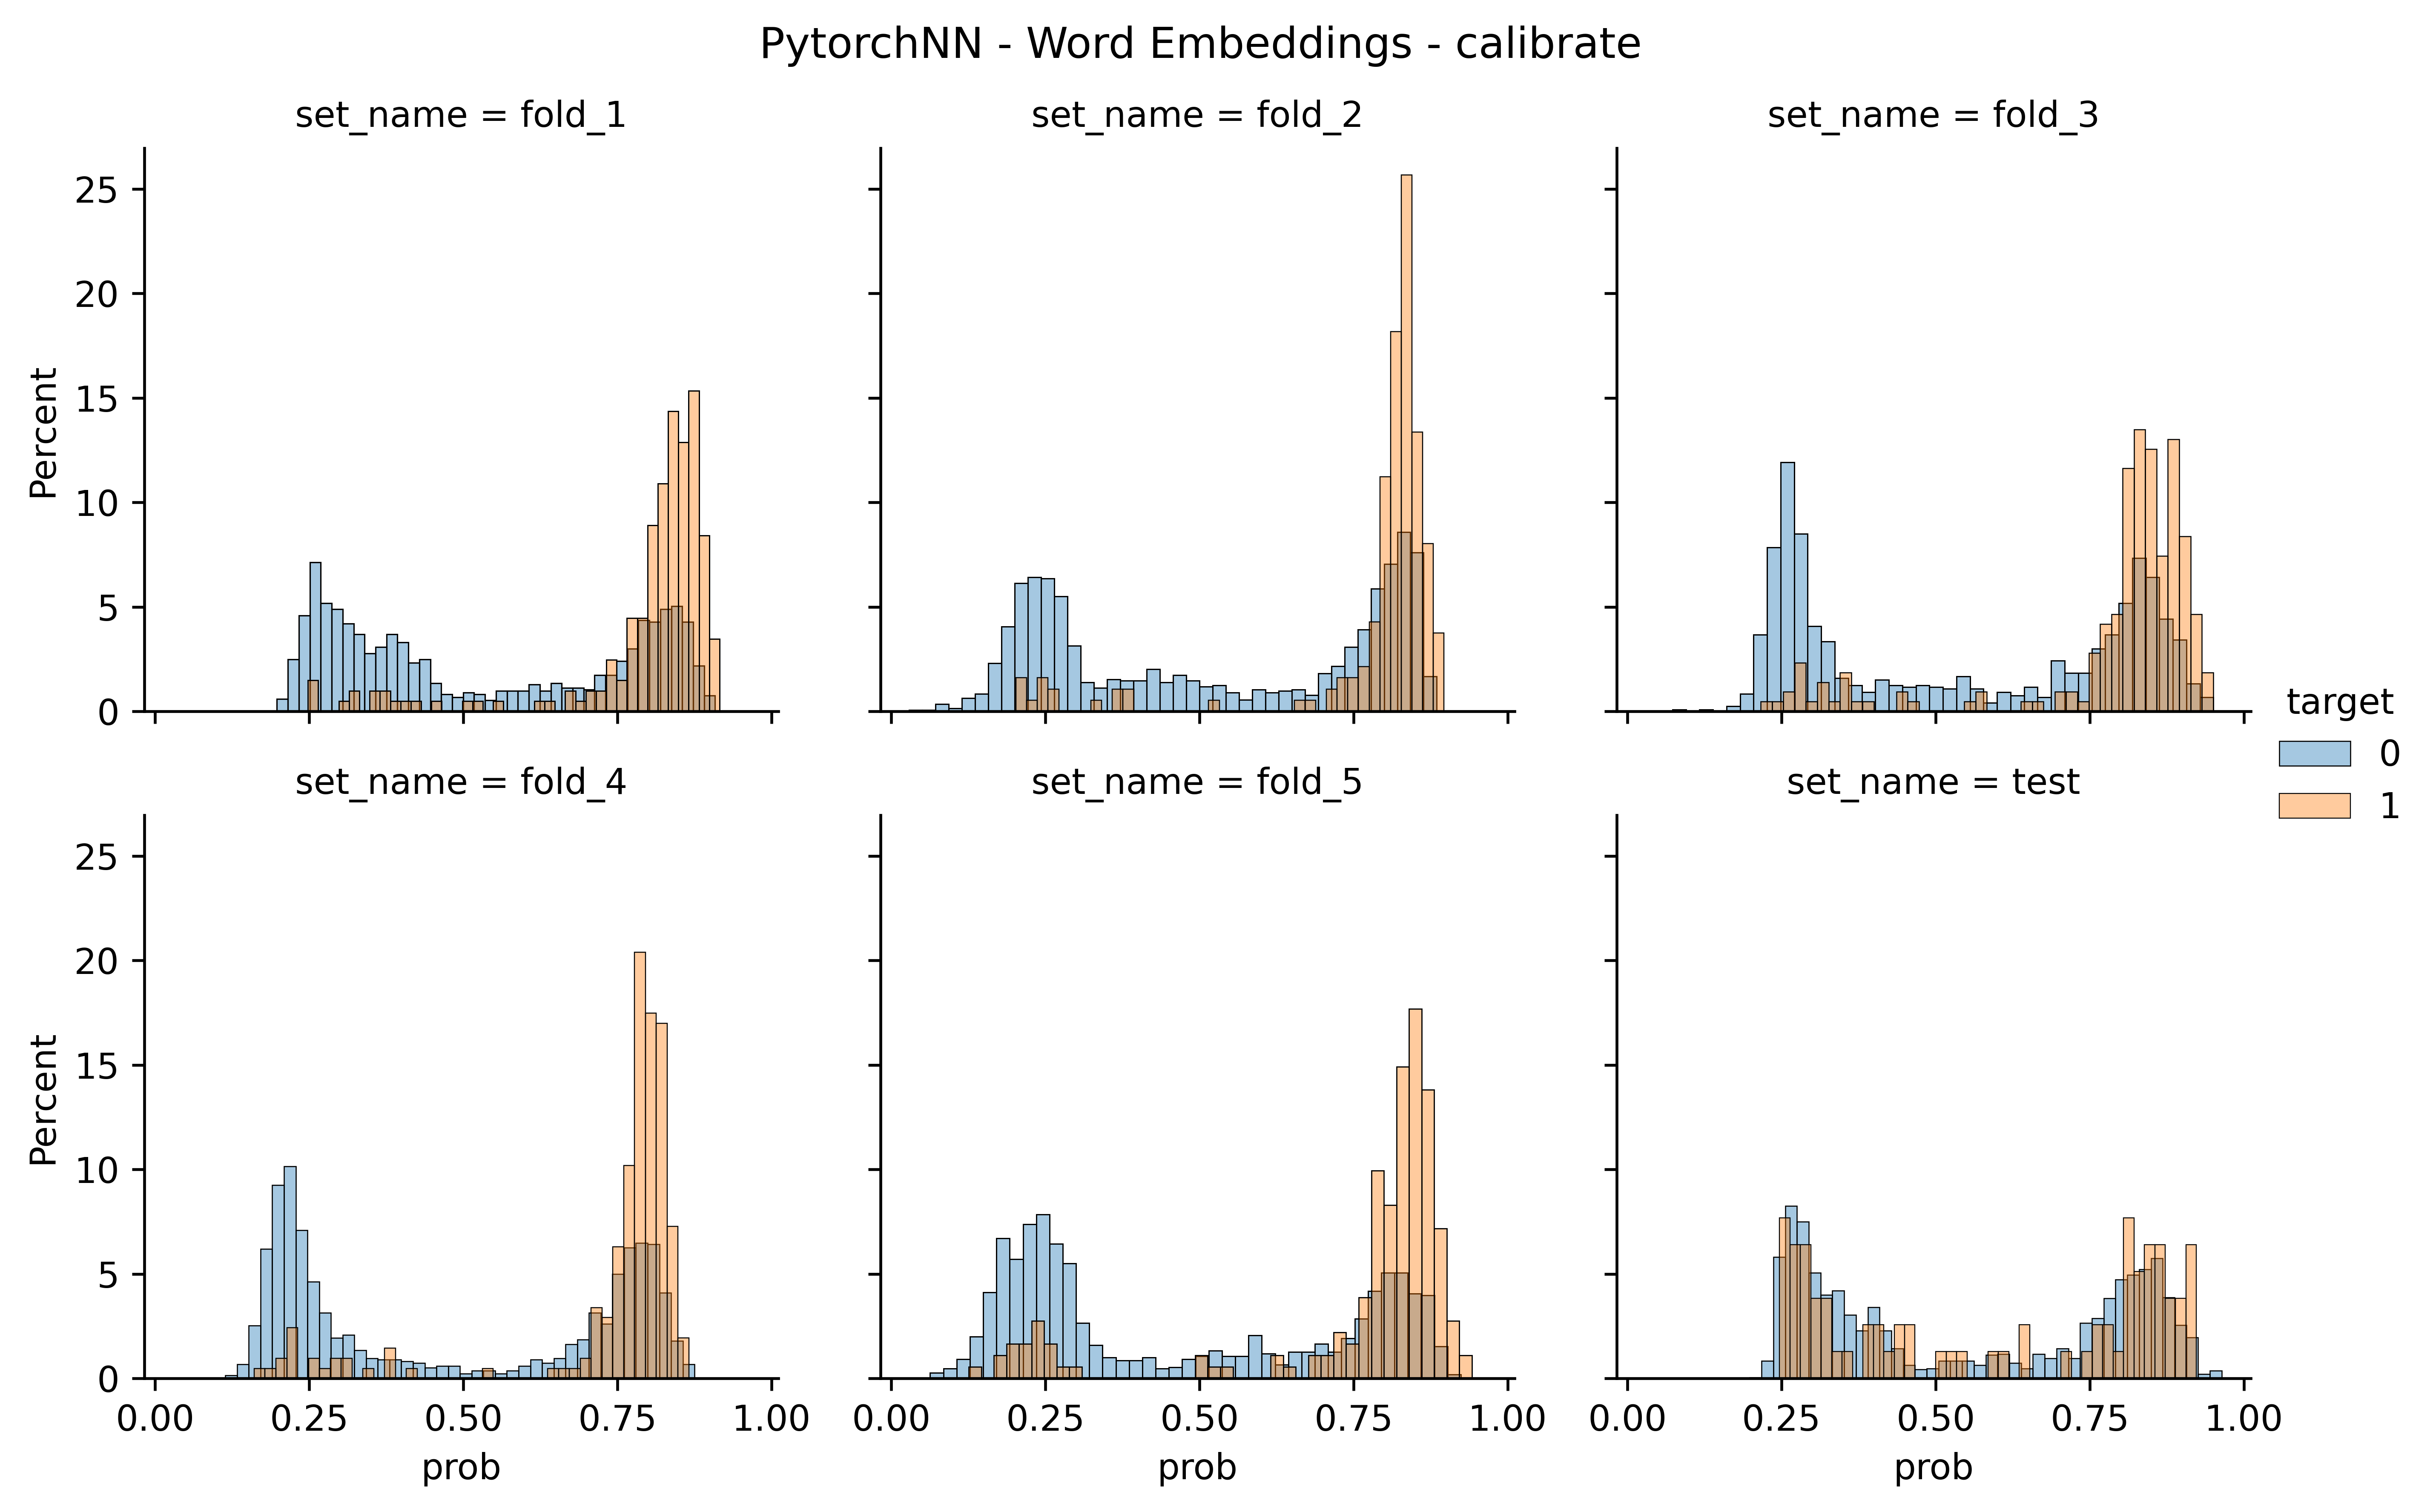
\includegraphics[width=\linewidth]{figures/results/word_embeddings/nn/calibrate/calibrate__distplot.png}
        \caption{Distribución de predicciones en validación cruzada y el conjunto de test.}
        \label{fig:my_label}
    \end{subfigure}
    \hfill
    \begin{subfigure}[b]{\textwidth}
    \minipage{0.32\textwidth}
      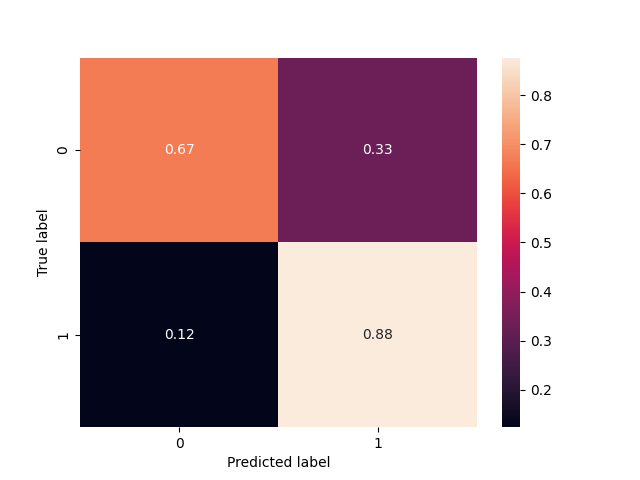
\includegraphics[width=\linewidth]{figures/results/word_embeddings/nn/calibrate/calibrate_set_1_confusion_matrix_percent.png}
    \endminipage\hfill
    \minipage{0.32\textwidth}
      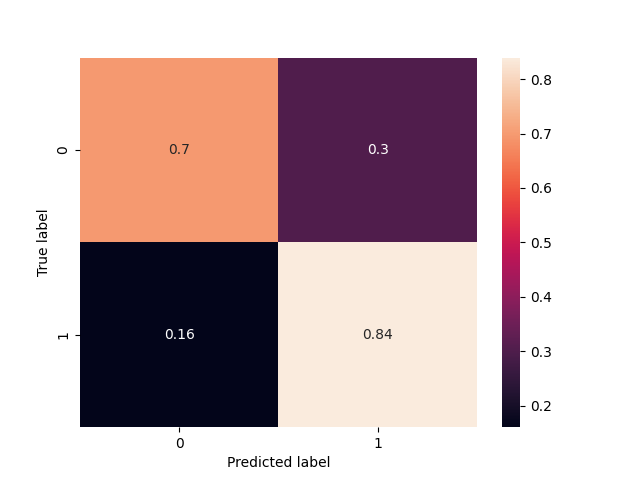
\includegraphics[width=\linewidth]{figures/results/word_embeddings/nn/calibrate/calibrate_set_2_confusion_matrix_percent.png}
    \endminipage\hfill \minipage{0.32\textwidth}%
      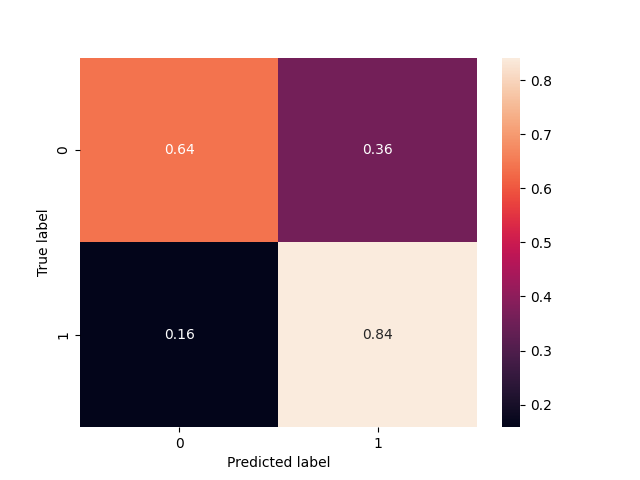
\includegraphics[width=\linewidth]{figures/results/word_embeddings/nn/calibrate/calibrate+_set_3_confusion_matrix_percent.png}
    \endminipage
    
    \medskip
    
    \minipage{0.32\textwidth}
      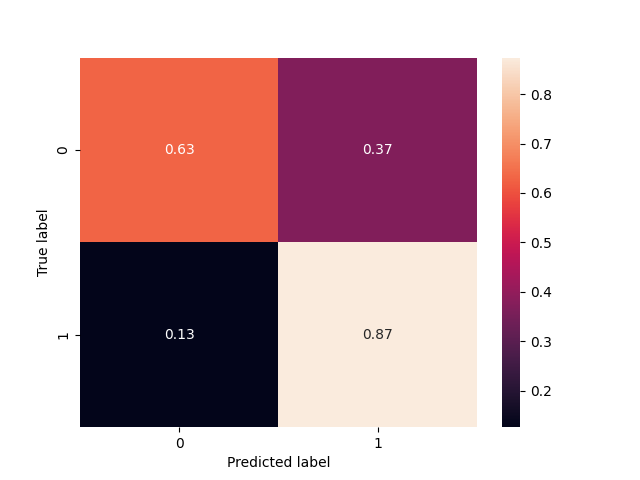
\includegraphics[width=\linewidth]{figures/results/word_embeddings/nn/calibrate/calibrate_set_4_confusion_matrix_percent.png}
    \endminipage\hfill
    \minipage{0.32\textwidth}
    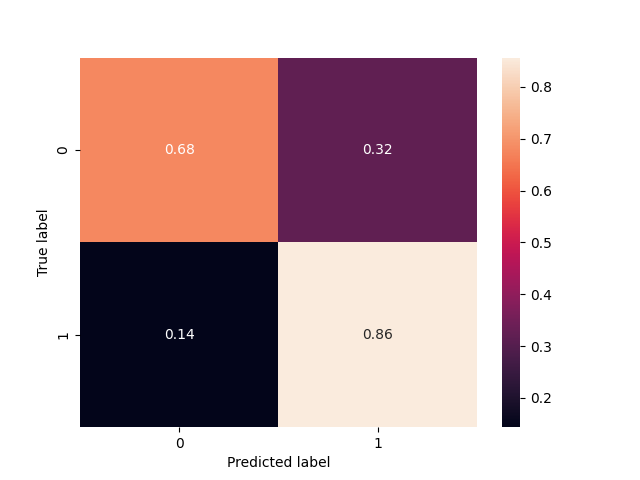
\includegraphics[width=\linewidth]{figures/results/word_embeddings/nn/calibrate/calibrate_set_5_confusion_matrix_percent.png}
    \endminipage\hfill \minipage{0.32\textwidth}%
    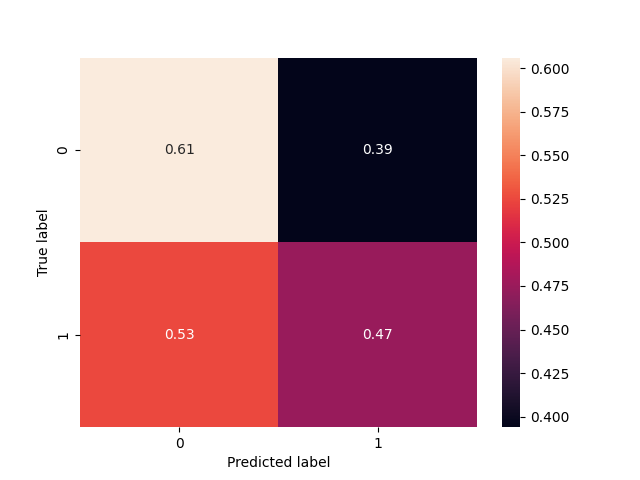
\includegraphics[width=\linewidth]{figures/results/word_embeddings/nn/calibrate/calibrate_set_6_confusion_matrix_percent.png}
    \endminipage
    \caption{Matrices de confusión en validación cruzada y el conjunto de test}
    \end{subfigure}
    \caption{Resultados del modelo de redes neuronales con codificación por word embeddings y esquema de acción calibrate.}
\end{figure}


\begin{figure}
    \begin{subfigure}[b]{\textwidth}
        \centering
        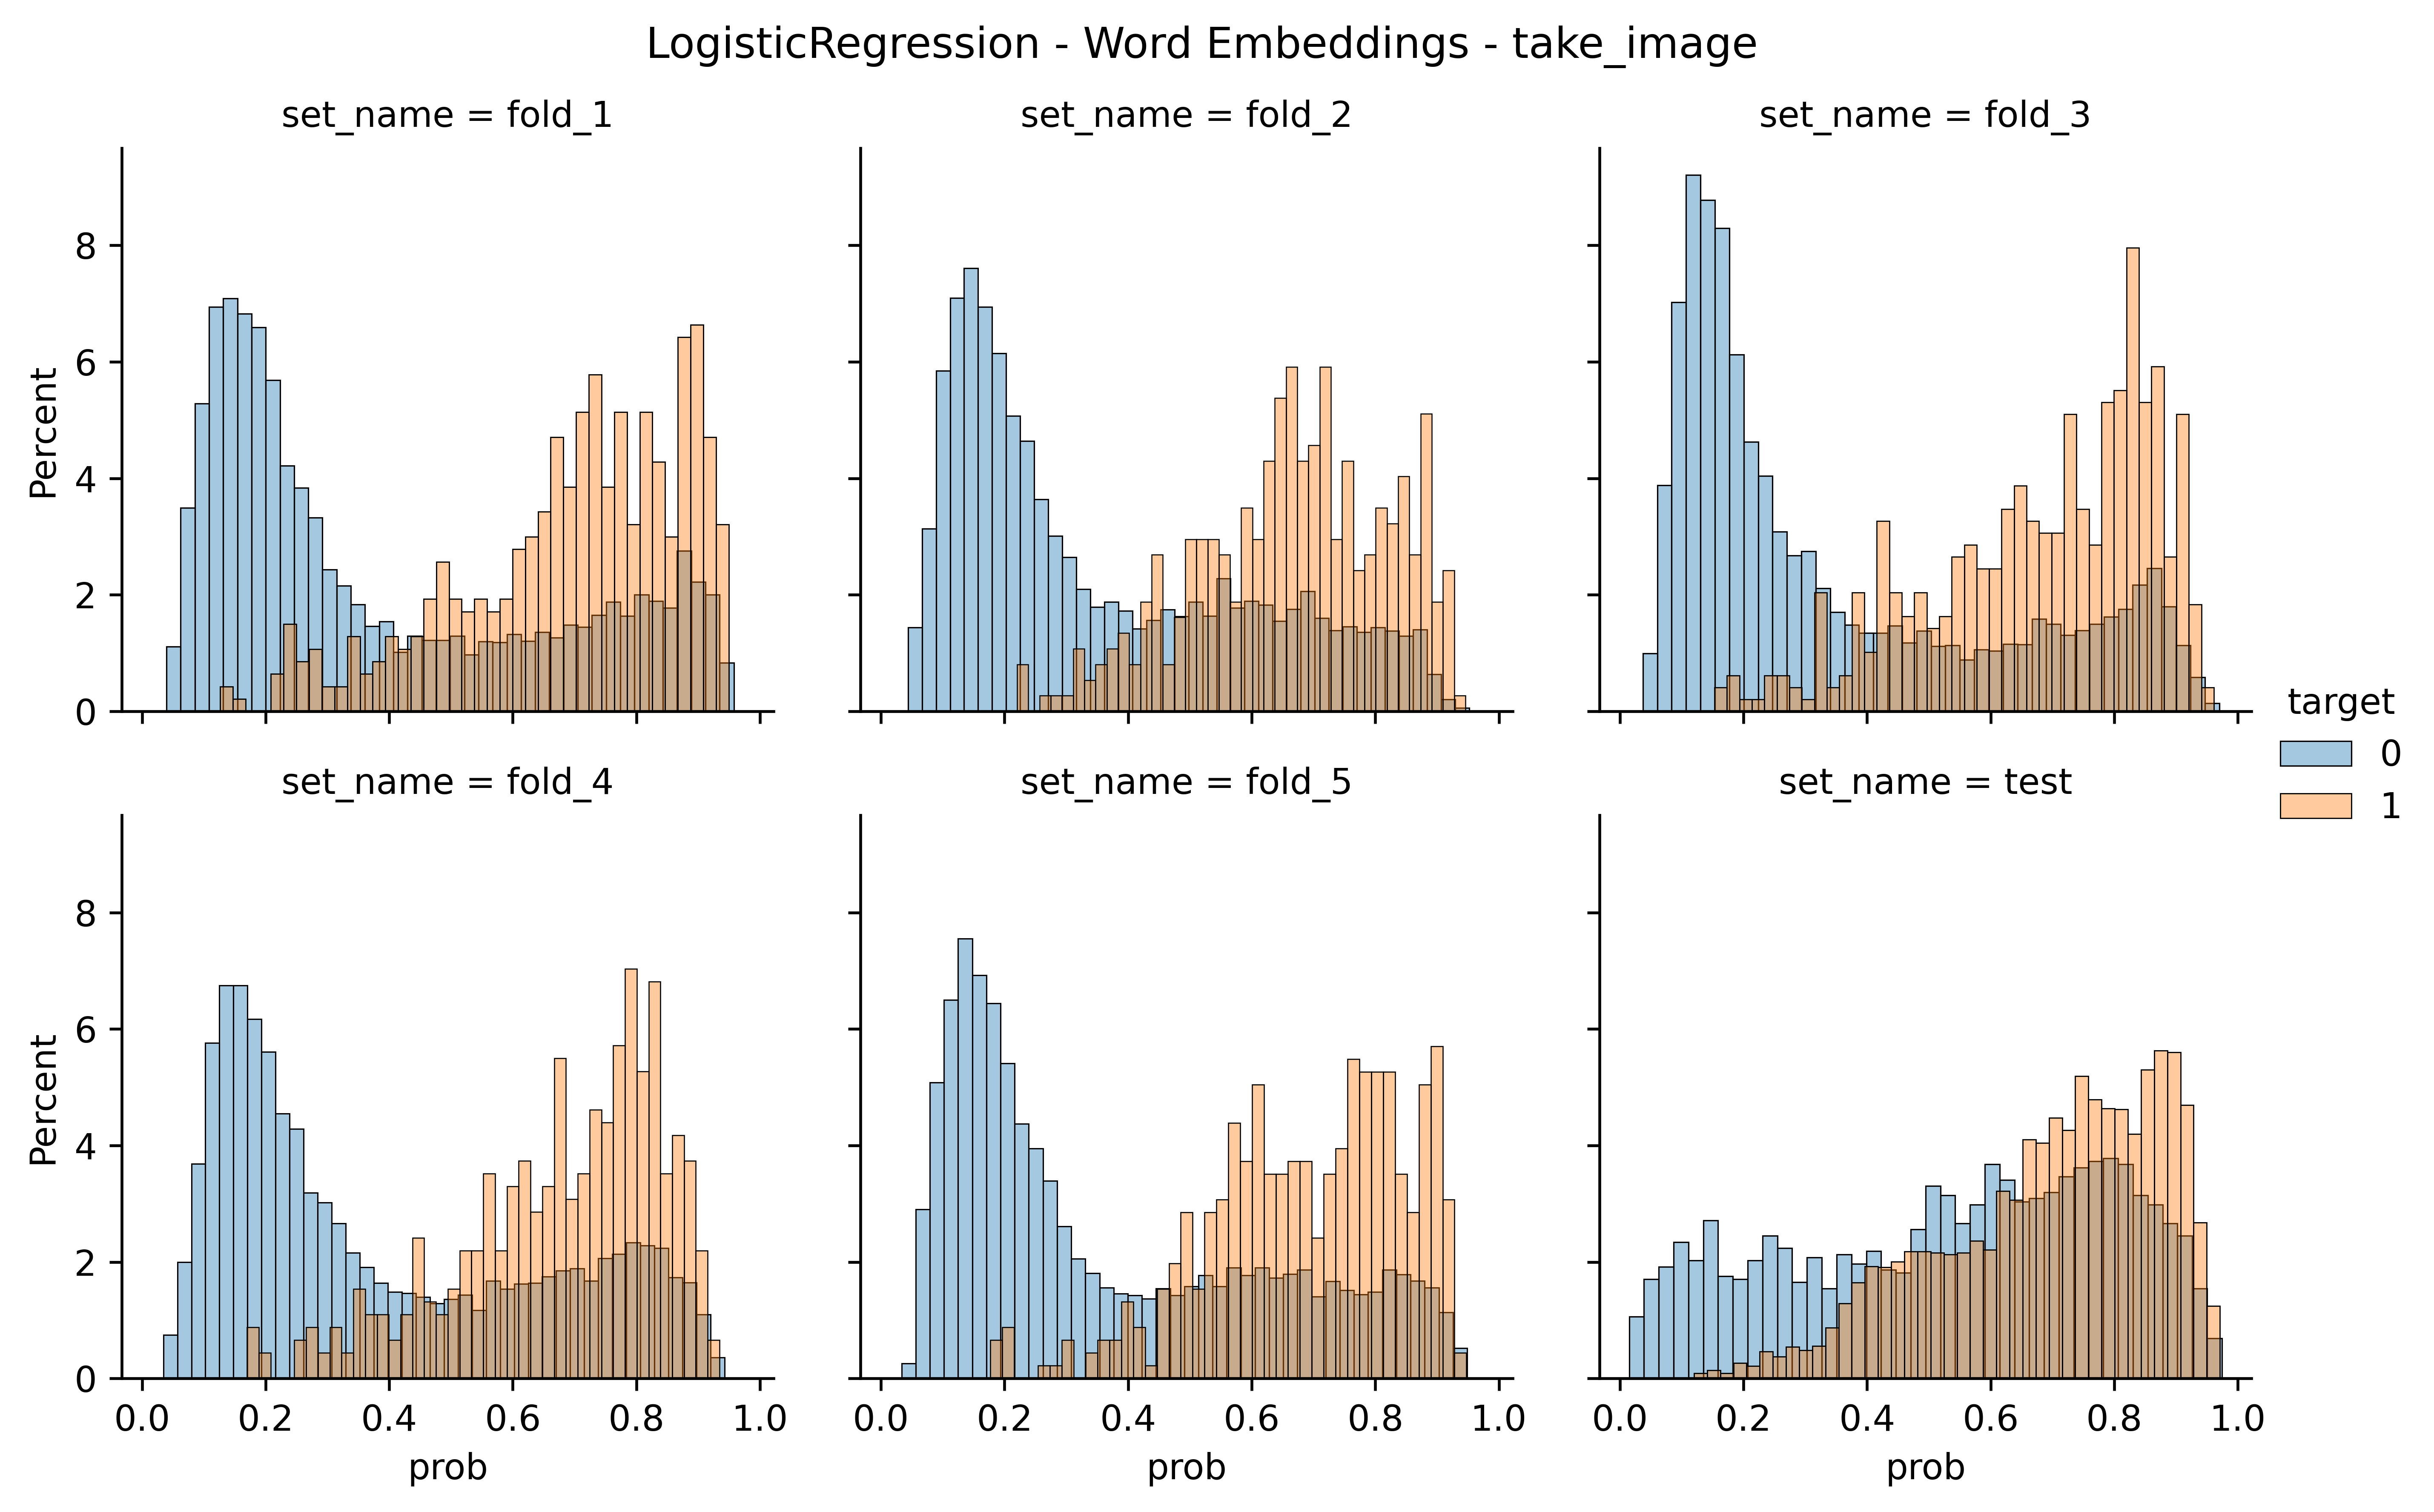
\includegraphics[width=\linewidth]{figures/results/word_embeddings/lgr/take_image/lgr__distplot.png}
        \caption{Distribución de predicciones en validación cruzada y el conjunto de test.}
        \label{fig:my_label}
    \end{subfigure}
    \hfill
    \begin{subfigure}[b]{\textwidth}
    \minipage{0.32\textwidth}
      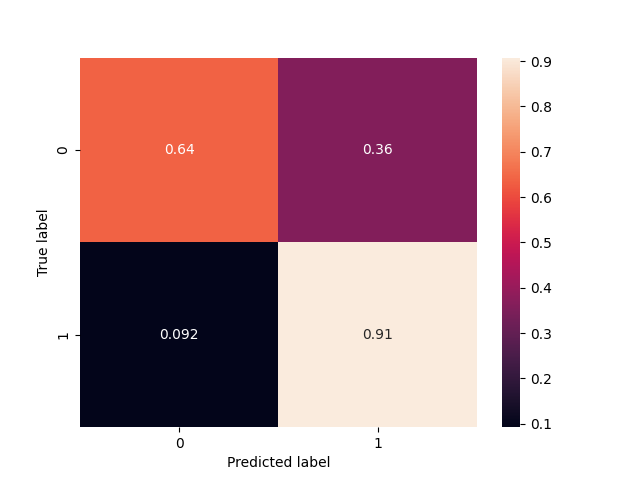
\includegraphics[width=\linewidth]{figures/results/word_embeddings/lgr/take_image/lgr_set_1_confusion_matrix_percent.png}
    \endminipage\hfill
    \minipage{0.32\textwidth}
      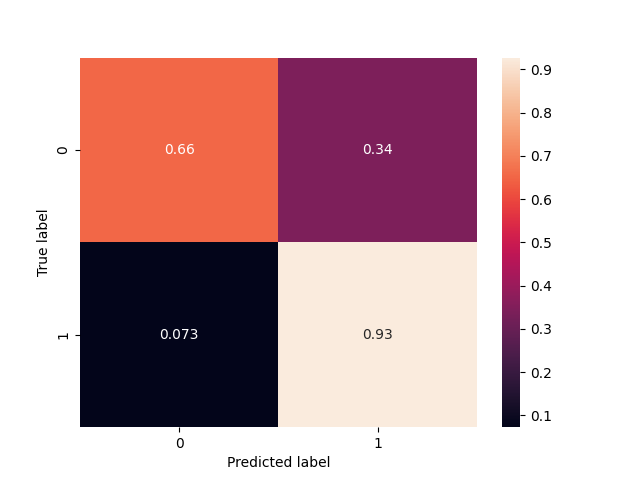
\includegraphics[width=\linewidth]{figures/results/word_embeddings/lgr/take_image/lgr_set_2_confusion_matrix_percent.png}
    \endminipage\hfill \minipage{0.32\textwidth}%
      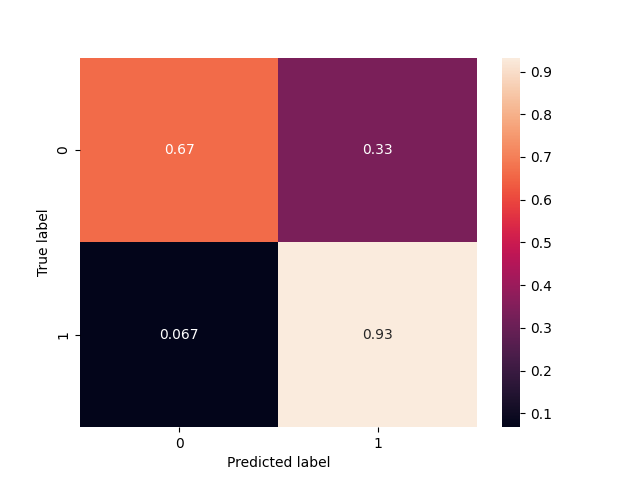
\includegraphics[width=\linewidth]{figures/results/word_embeddings/lgr/take_image/lgr_set_3_confusion_matrix_percent.png}
    \endminipage
    
    \medskip
    
    \minipage{0.32\textwidth}
      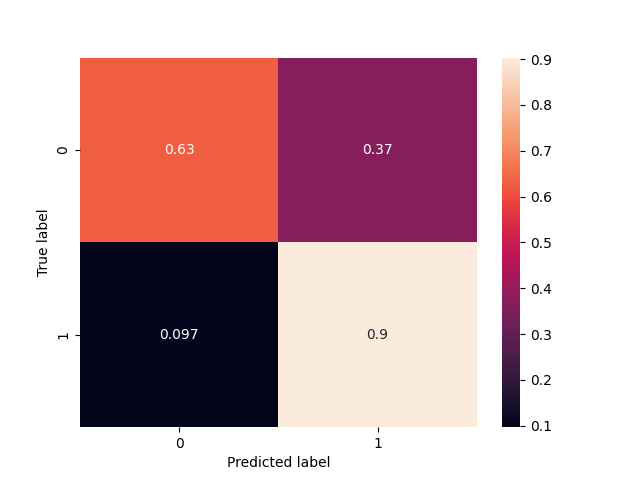
\includegraphics[width=\linewidth]{figures/results/word_embeddings/lgr/take_image/lgr_set_4_confusion_matrix_percent.png}
    \endminipage\hfill
    \minipage{0.32\textwidth}
      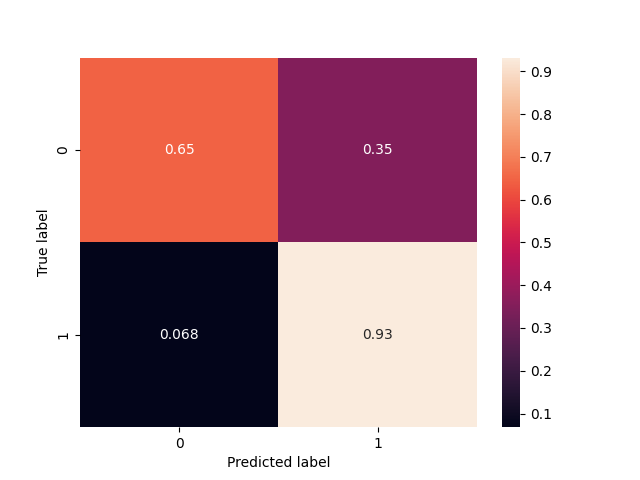
\includegraphics[width=\linewidth]{figures/results/word_embeddings/lgr/take_image/lgr_set_5_confusion_matrix_percent.png}
    \endminipage\hfill \minipage{0.32\textwidth}%
      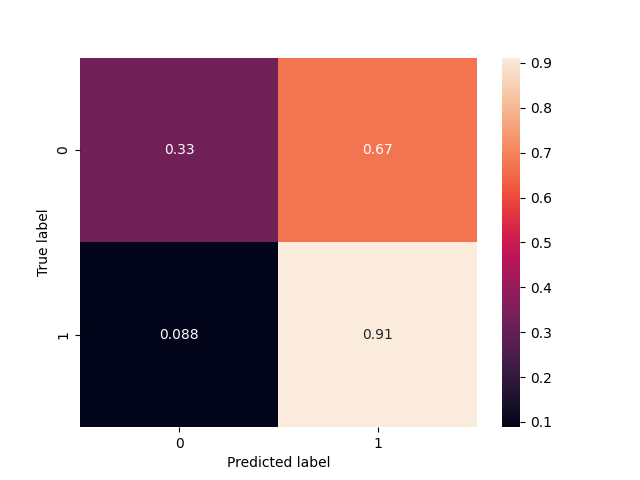
\includegraphics[width=\linewidth]{figures/results/word_embeddings/lgr/take_image/lgr_set_6_confusion_matrix_percent.png}
    \endminipage
    \caption{Matrices de confusión en validación cruzada y el conjunto de test}
    \end{subfigure}
    \caption{Resultados del modelo de regresión logística con codificación por word embeddings y esquema de acción take\_image.}
\end{figure}


\begin{figure}
    \centering
    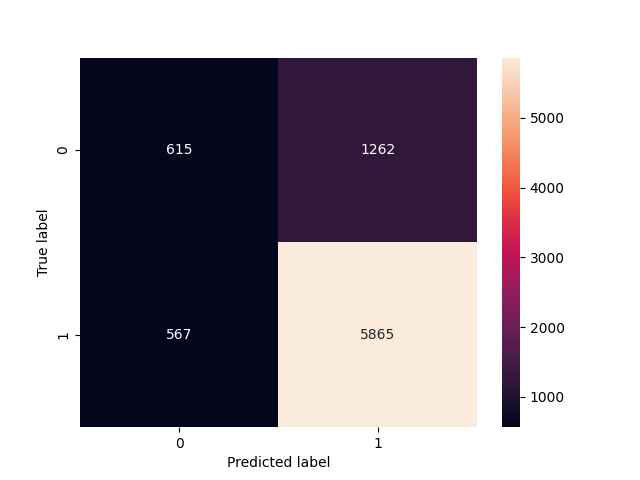
\includegraphics[scale=0.7]{figures/results/word_embeddings/lgr/take_image/lgr_set_6_confusion_matrix_raw.png}
    \caption{Matriz de confusión sin porcentajes del modelo de regresión logística con codificación por word embeddings y esquema de acción take\_image.}
    \label{fig:my_label}
\end{figure}

\begin{table}[h!]
\centering
\scalebox{0.9}{
 \begin{tabular}{|c || c | c | c | c | c | c |} 
 \hline
  Esquemas & Precisión & Recall & $H_{1.5}$ & $F_{1.5}$ & Umbral de decisión &
  Modelo \\
 \hline
 take\_image & 0.8088 & 0.997 & 0.4351 & 0.997 & 0.61 & LGR \\
 calibrate & 0.0467 & 0.4743 & 0.5083 & 0.1242 & 0.728 & NN\\
 switch\_on  & 0.0405 & 0.4567 & 0.5106 & 0.1097 & 0.576 & NN\\
 switch\_off & 0.0476 & 0.1818 & 0.2422 & 0.0876 & 0.034 & NN \\
 turn\_to  & - & - & - & - & - & -\\[1ex]
 \hline
 \end{tabular}}
 \caption{Resultados por esquema de acción del mejor modelo con codificación por word embeddings.}
 \label{results:ad-hoc-calibrate}
\end{table}


\section{Modelos predictivos ad-hoc}
\label{exp:wb}

\subsection{Configuración del experimento}

Como contraparte del experimento anterior, usaremos la codificación por word
embeddings, bajo el mismo conjunto de entrenamientos y construcción de ventanas,
con la salvedad de ser codificados a partir del modelo de lenguaje de FastText,
entrenado con oraciones provenientes de planes relajados. El modelo de lenguaje
es un modelo Skipgram entrenado por $100$ épocas, un tamaño de ventana de
contexto de $3$ palabras, y un vector de salida de dimensión $30$. Se hicieron
pruebas sobre otras configuraciones de parámetros pero el comportamiento que
buscábamos que el modelo de lenguaje aprendiese ya era obtenido bajo esta
configuración.

Los clasificadores y grillas de búsqueda de parámetros utilizadas fueron las
mismos que los modelo predictivos ad-hoc.

\subsection{Resultados}

\begin{figure}
    \centering
    \begin{subfigure}[b]{0.83\textwidth}
    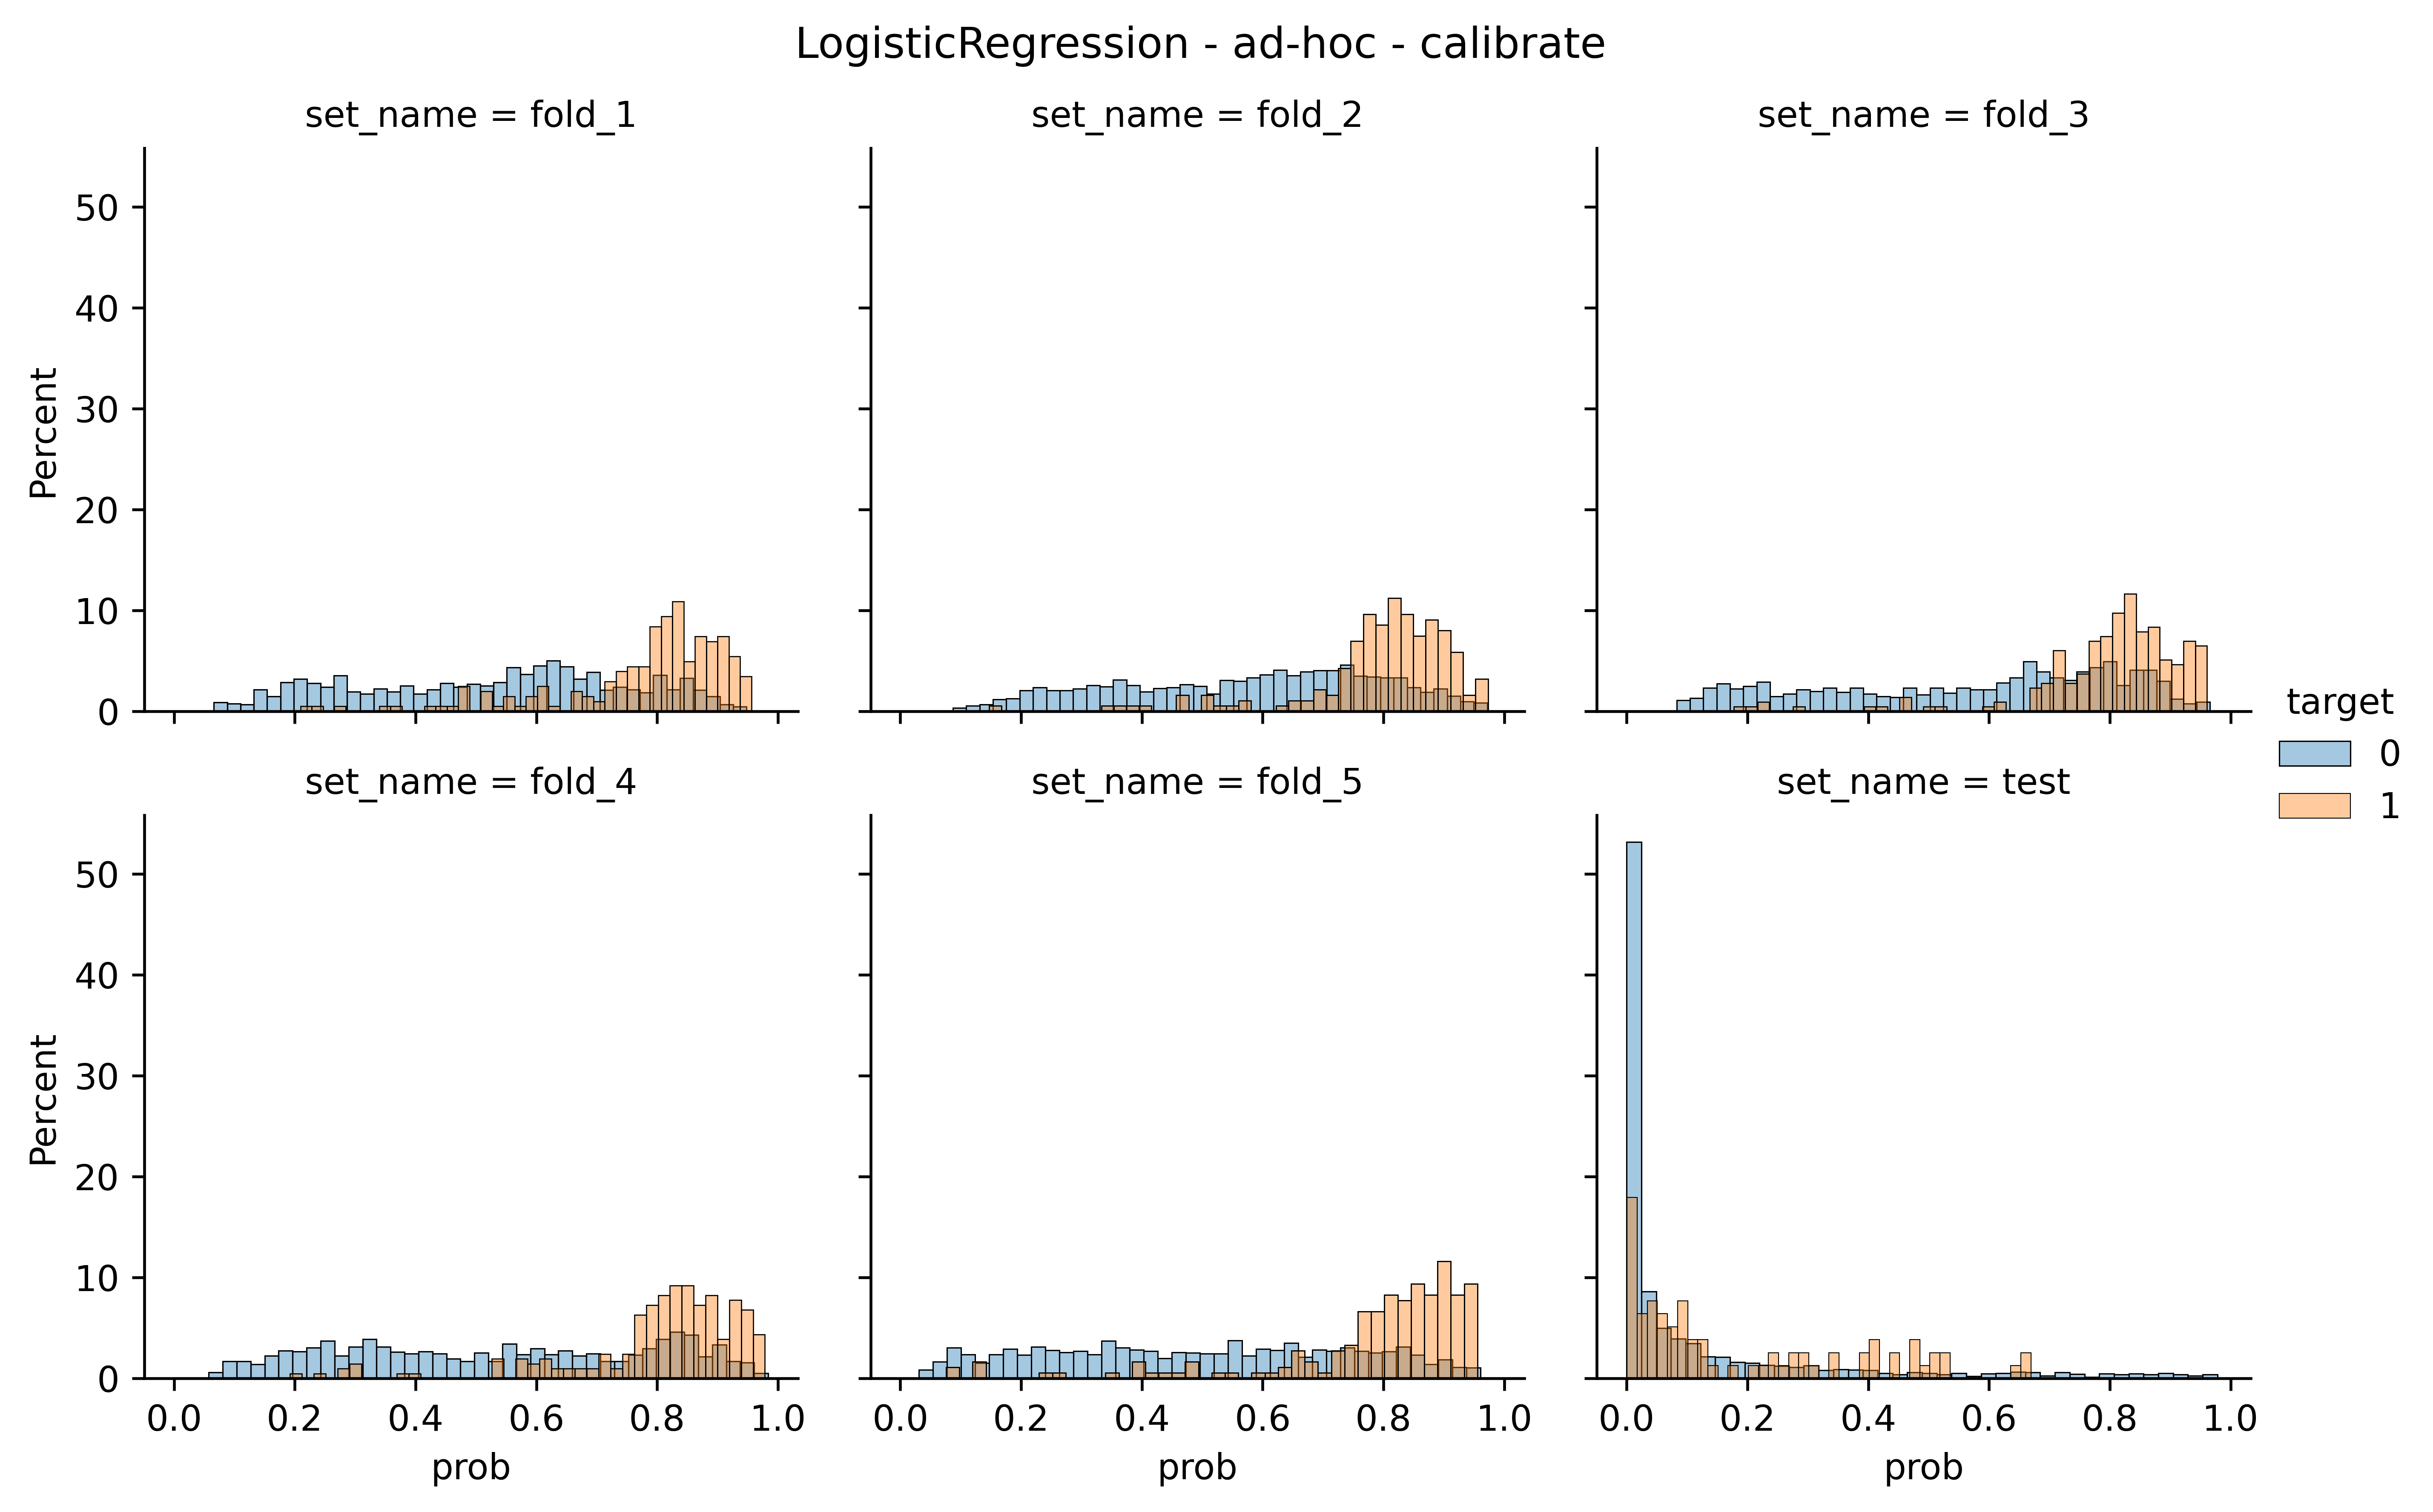
\includegraphics[width=\linewidth]{figures/results/ad-hoc/lgr/calibrate/calibrate__distplot.png}
    \end{subfigure}
    \hfill
    \centering
    \begin{subfigure}[b]{0.83\textwidth}
        \centering
        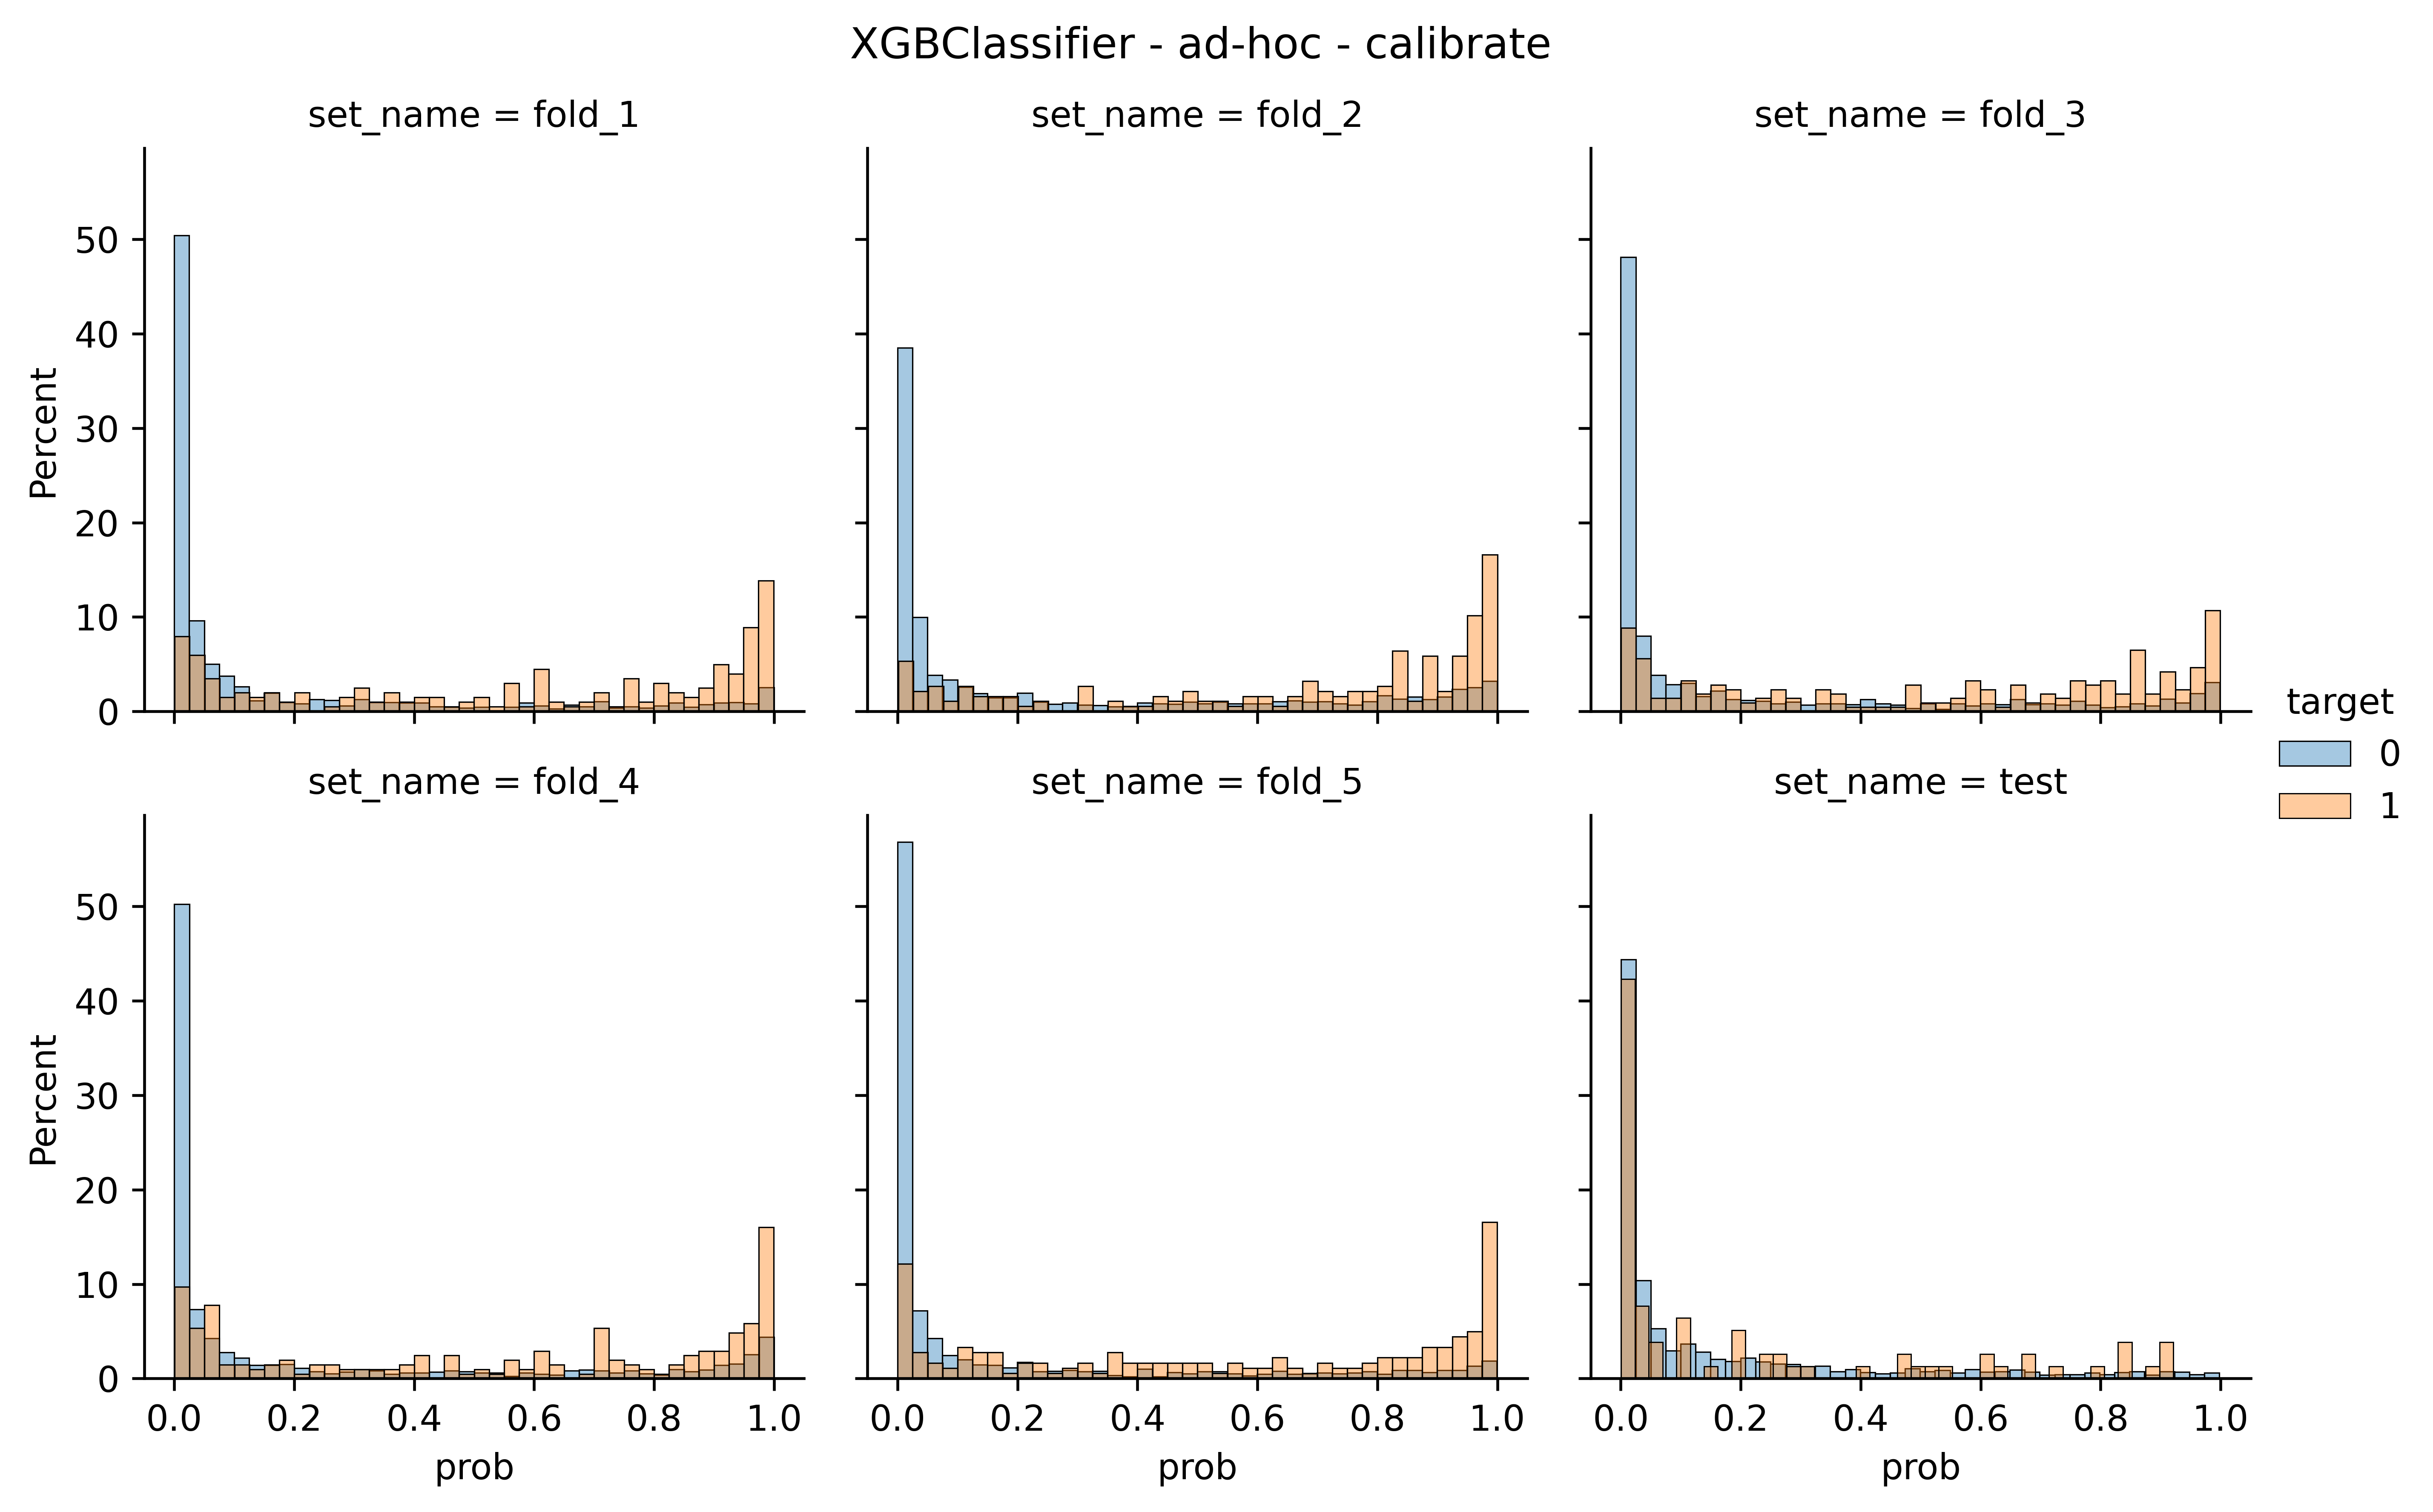
\includegraphics[width=\linewidth]{figures/results/ad-hoc/xgb/2021-12-07_06.29.19.600877__distplot (2).png}
    \end{subfigure}
    \hfill
    \centering
    \begin{subfigure}[b]{0.83\textwidth}
        \centering
        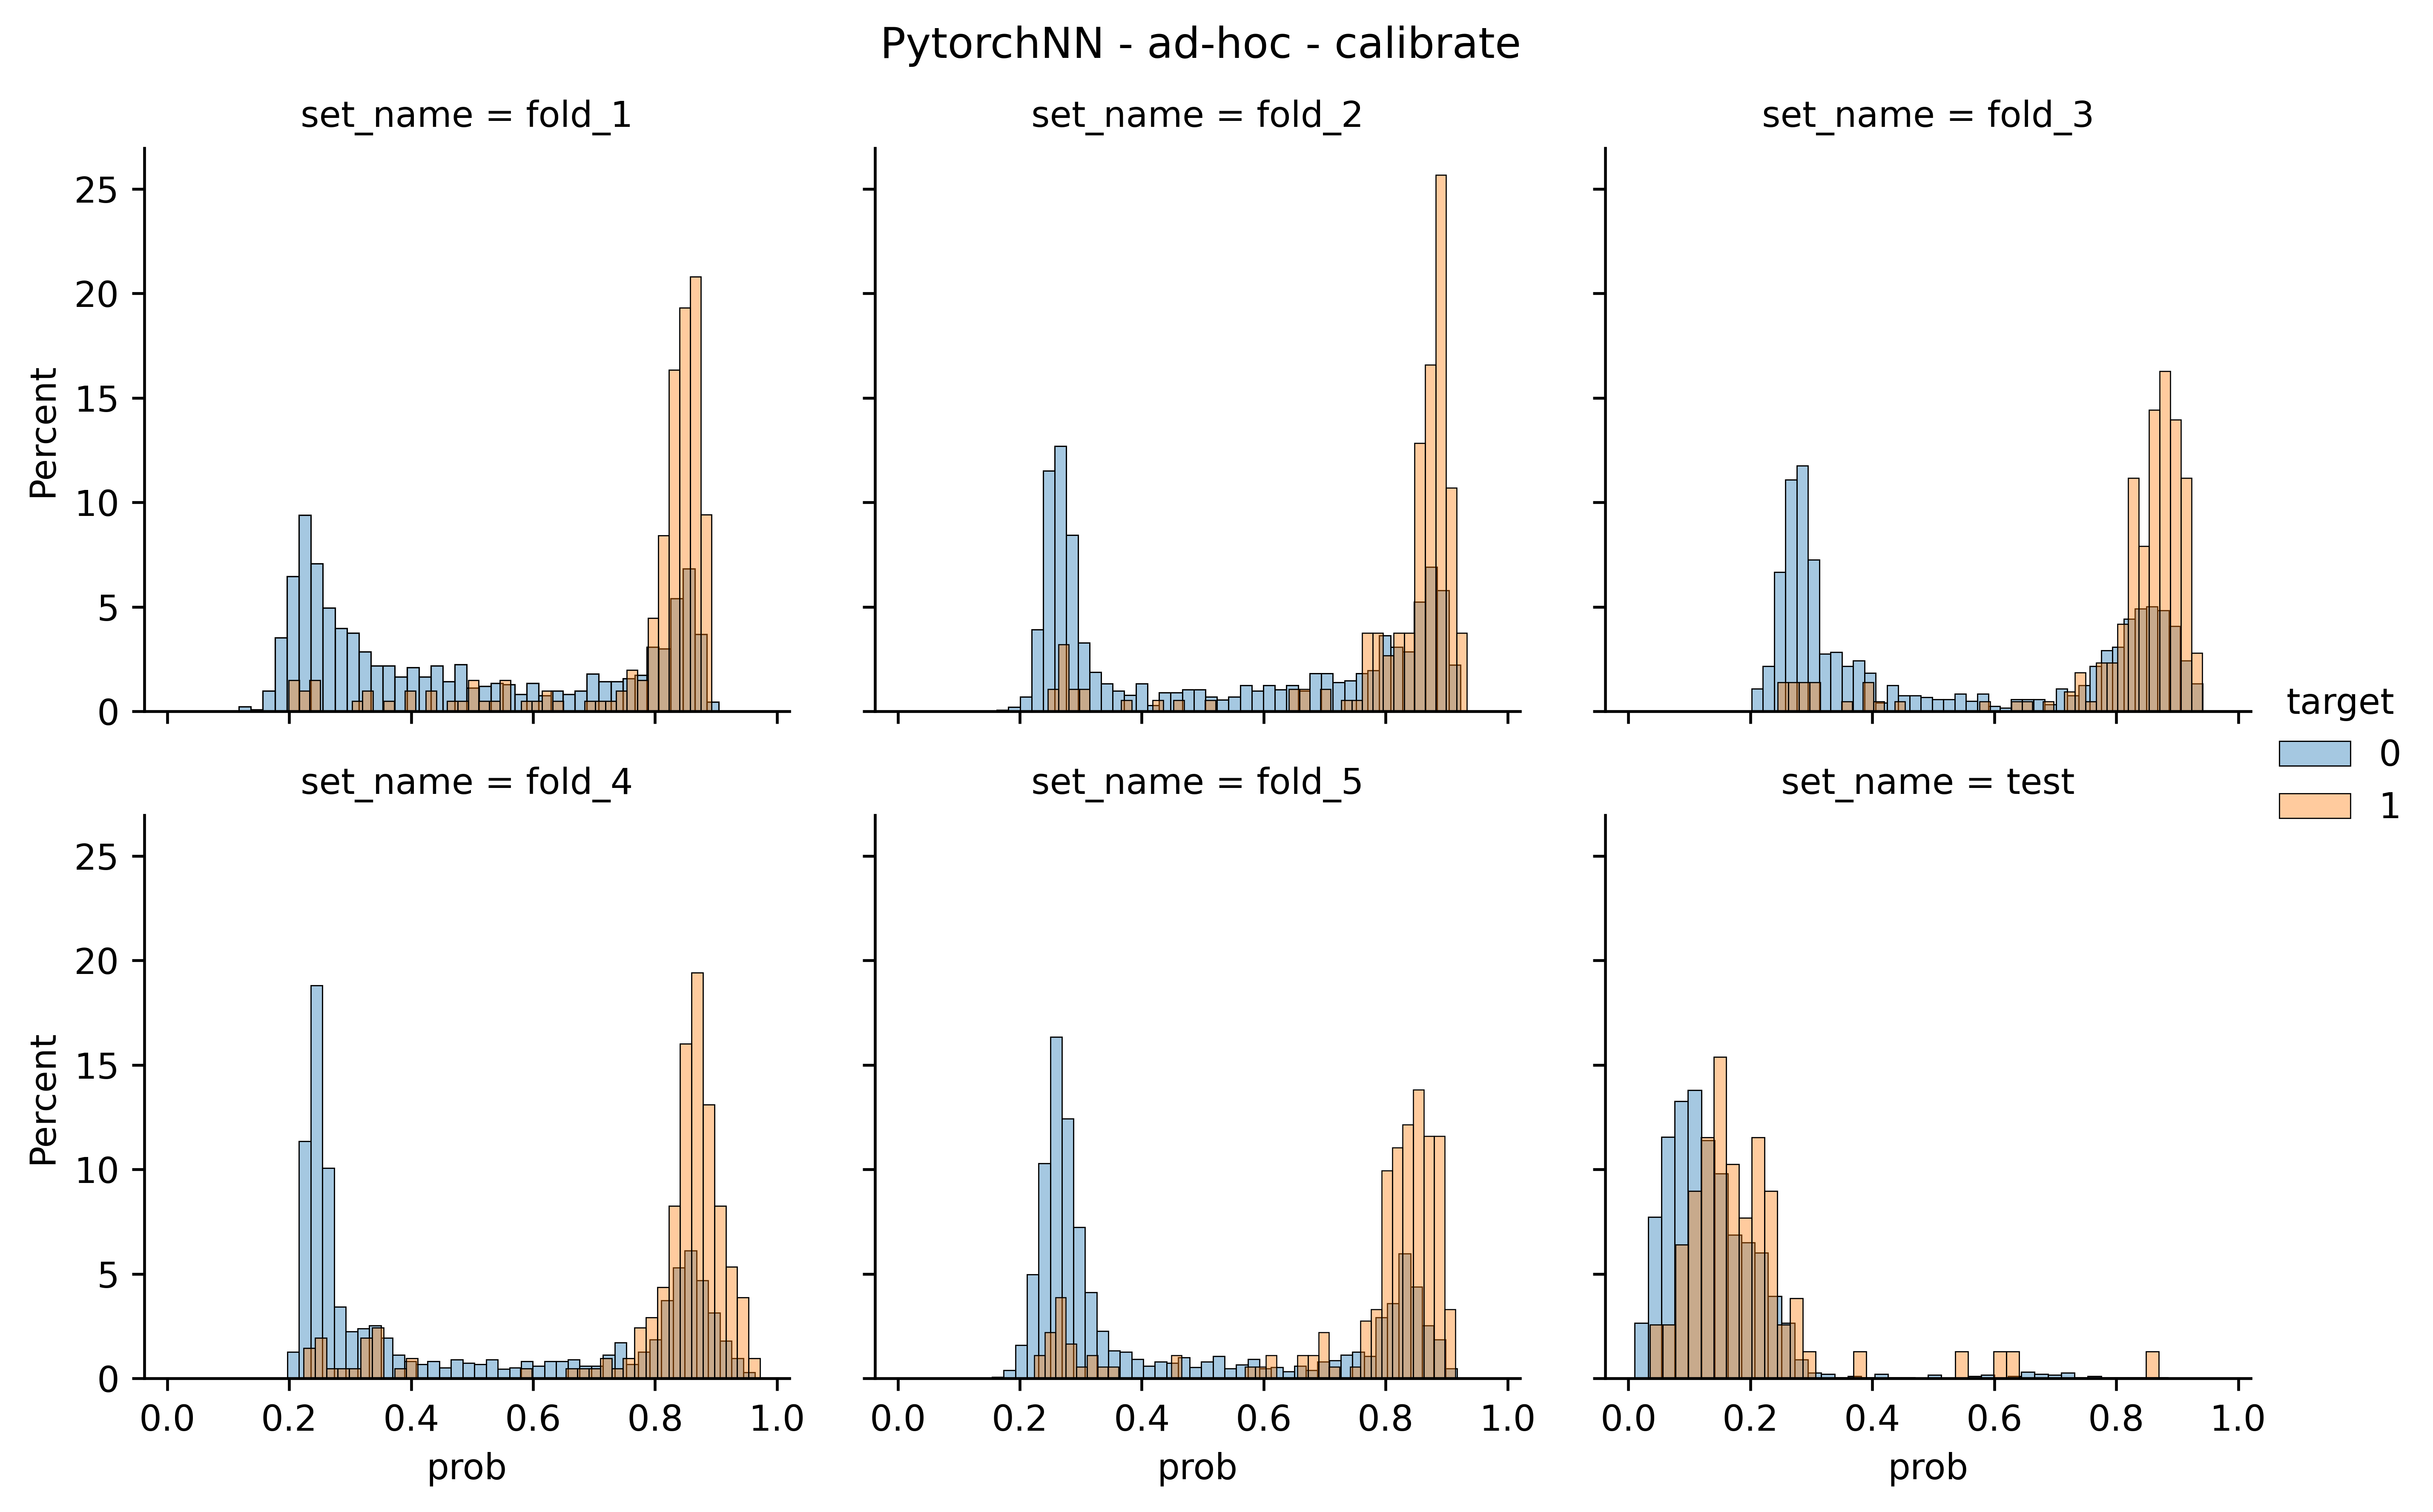
\includegraphics[width=\linewidth]{figures/results/ad-hoc/nn/2021-12-06_17.03.17.314982__distplot.png}
    \end{subfigure}
    \caption{Ad-hoc calibrate}
\end{figure}

\begin{figure}
    \centering
    \begin{subfigure}[b]{0.83\textwidth}
    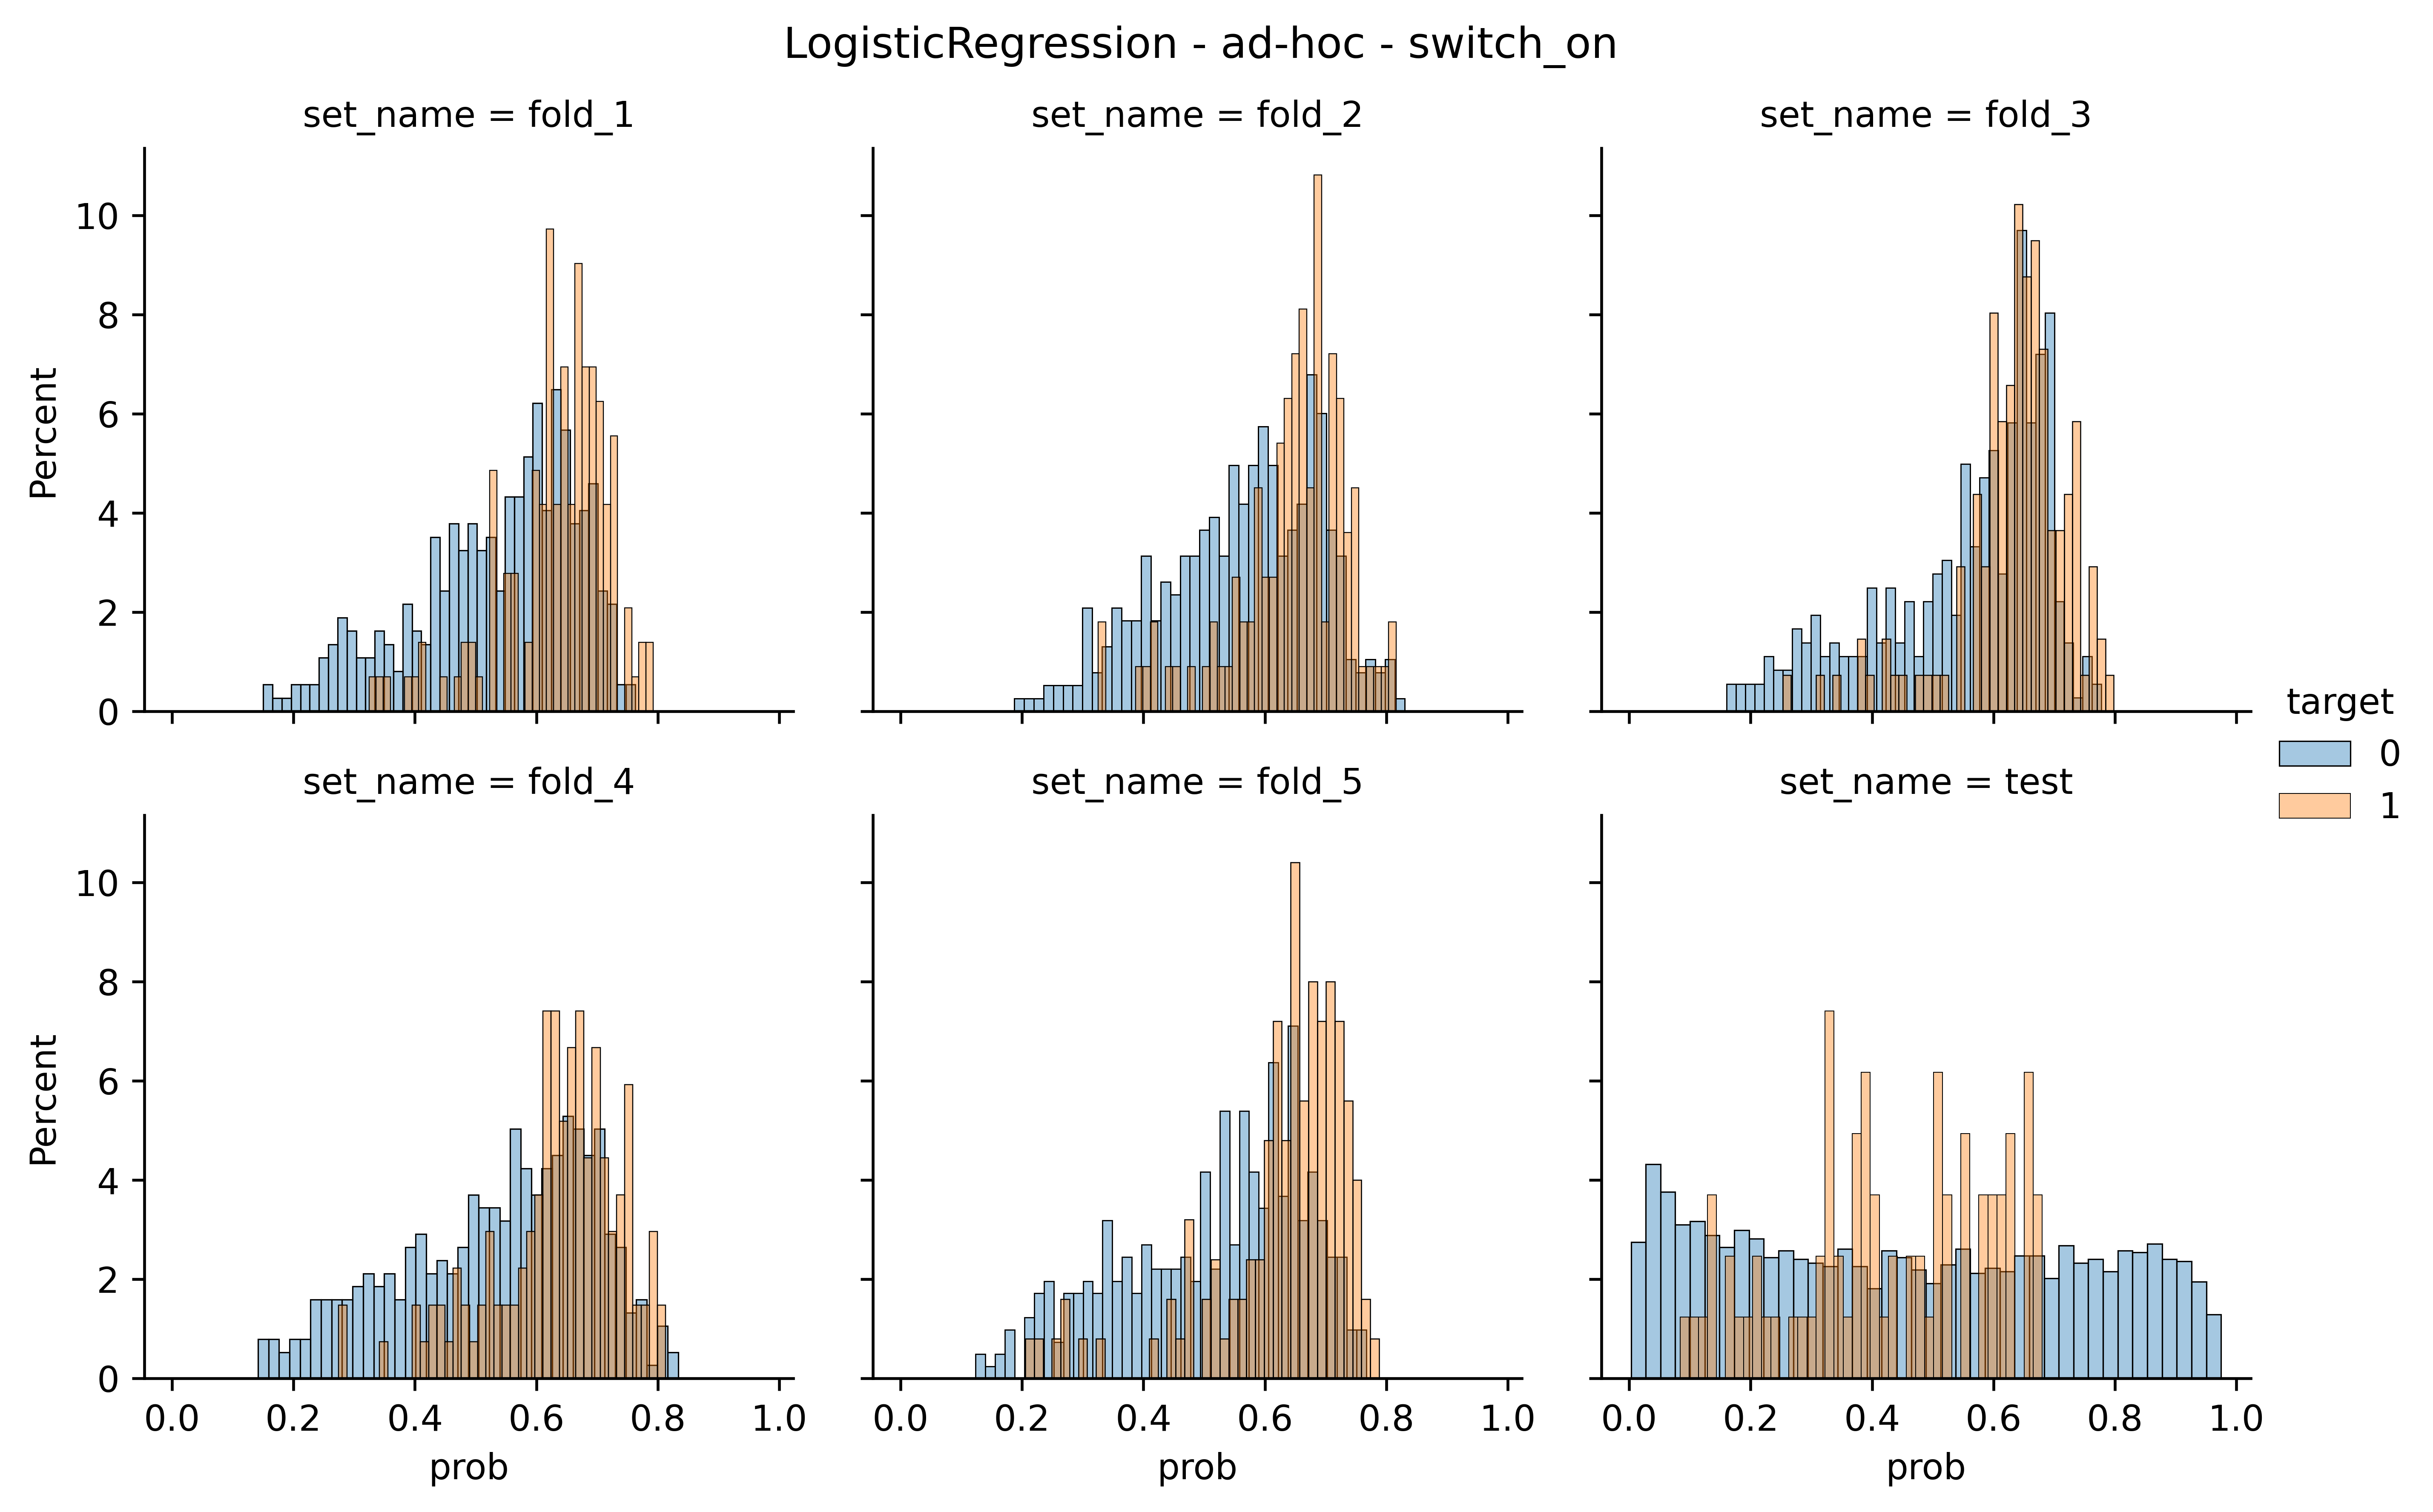
\includegraphics[width=\linewidth]{figures/results/ad-hoc/lgr/switch_on/turn_to__distplot.png}
    \end{subfigure}
    \hfill
    \centering
    \begin{subfigure}[b]{0.83\textwidth}
        \centering
        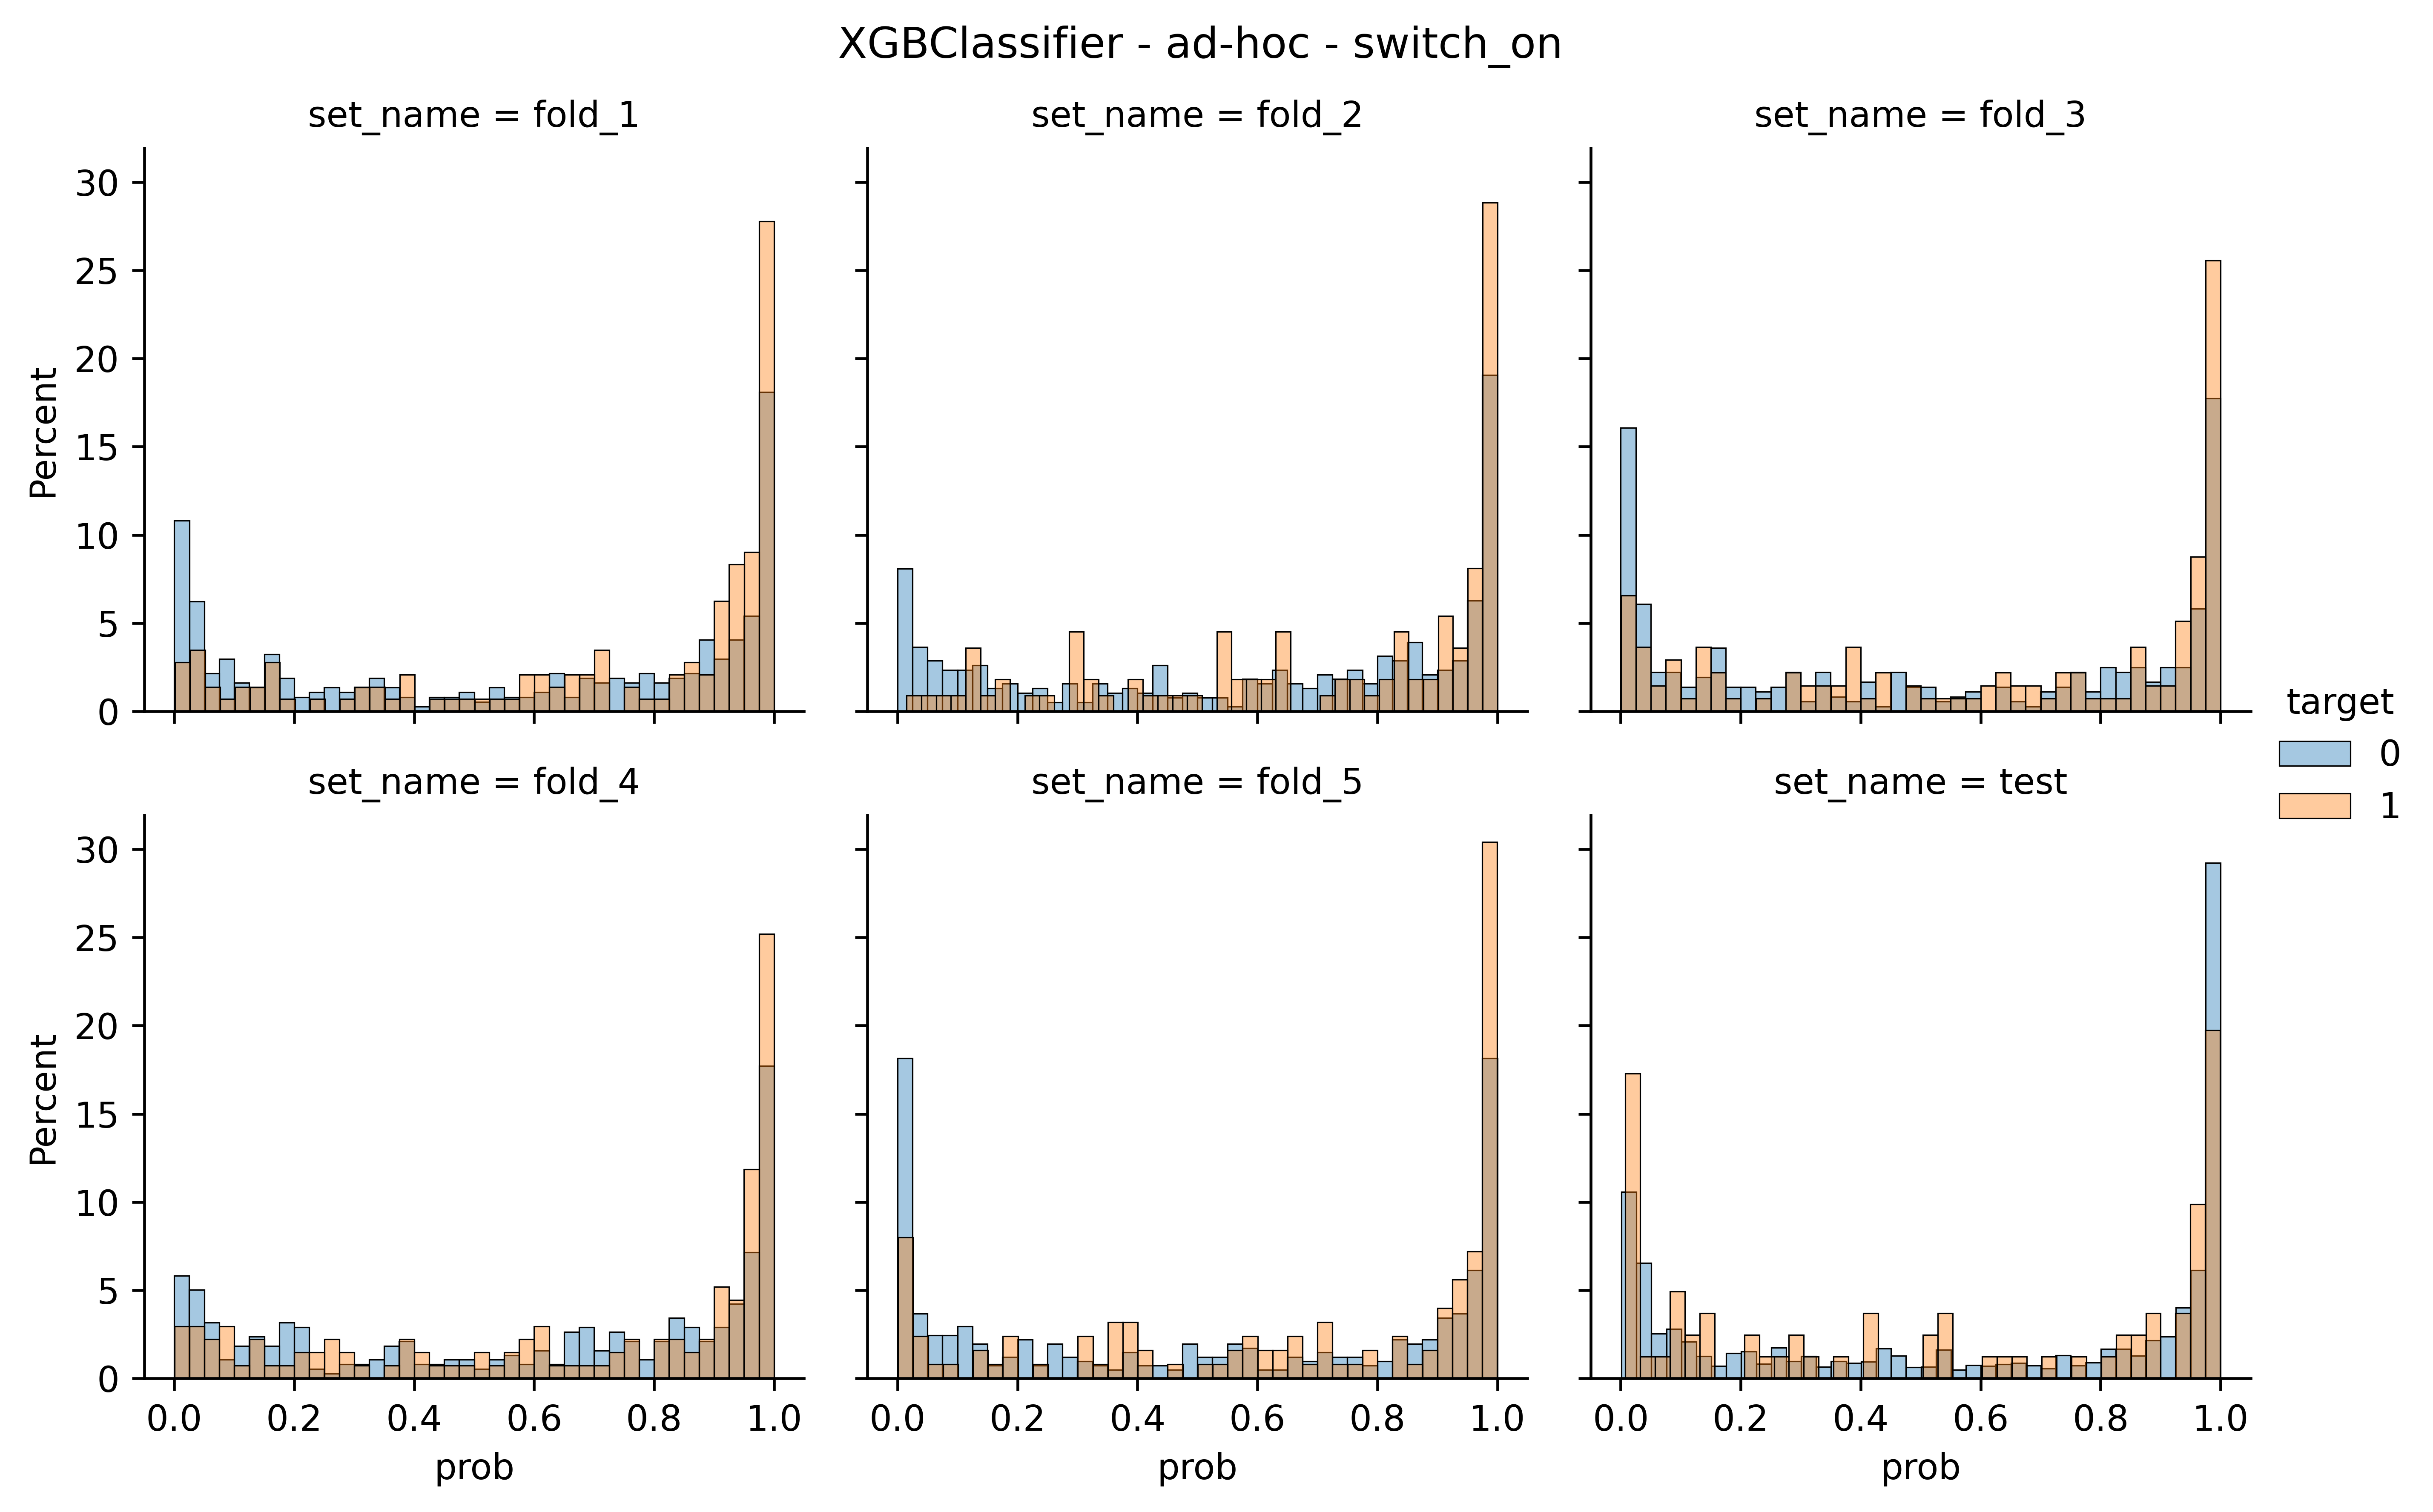
\includegraphics[width=\linewidth]{figures/results/ad-hoc/xgb/switch_on/2021-12-07_06.56.08.418411__distplot.png}
    \end{subfigure}
    \hfill
    \centering
    \begin{subfigure}[b]{0.83\textwidth}
        \centering
        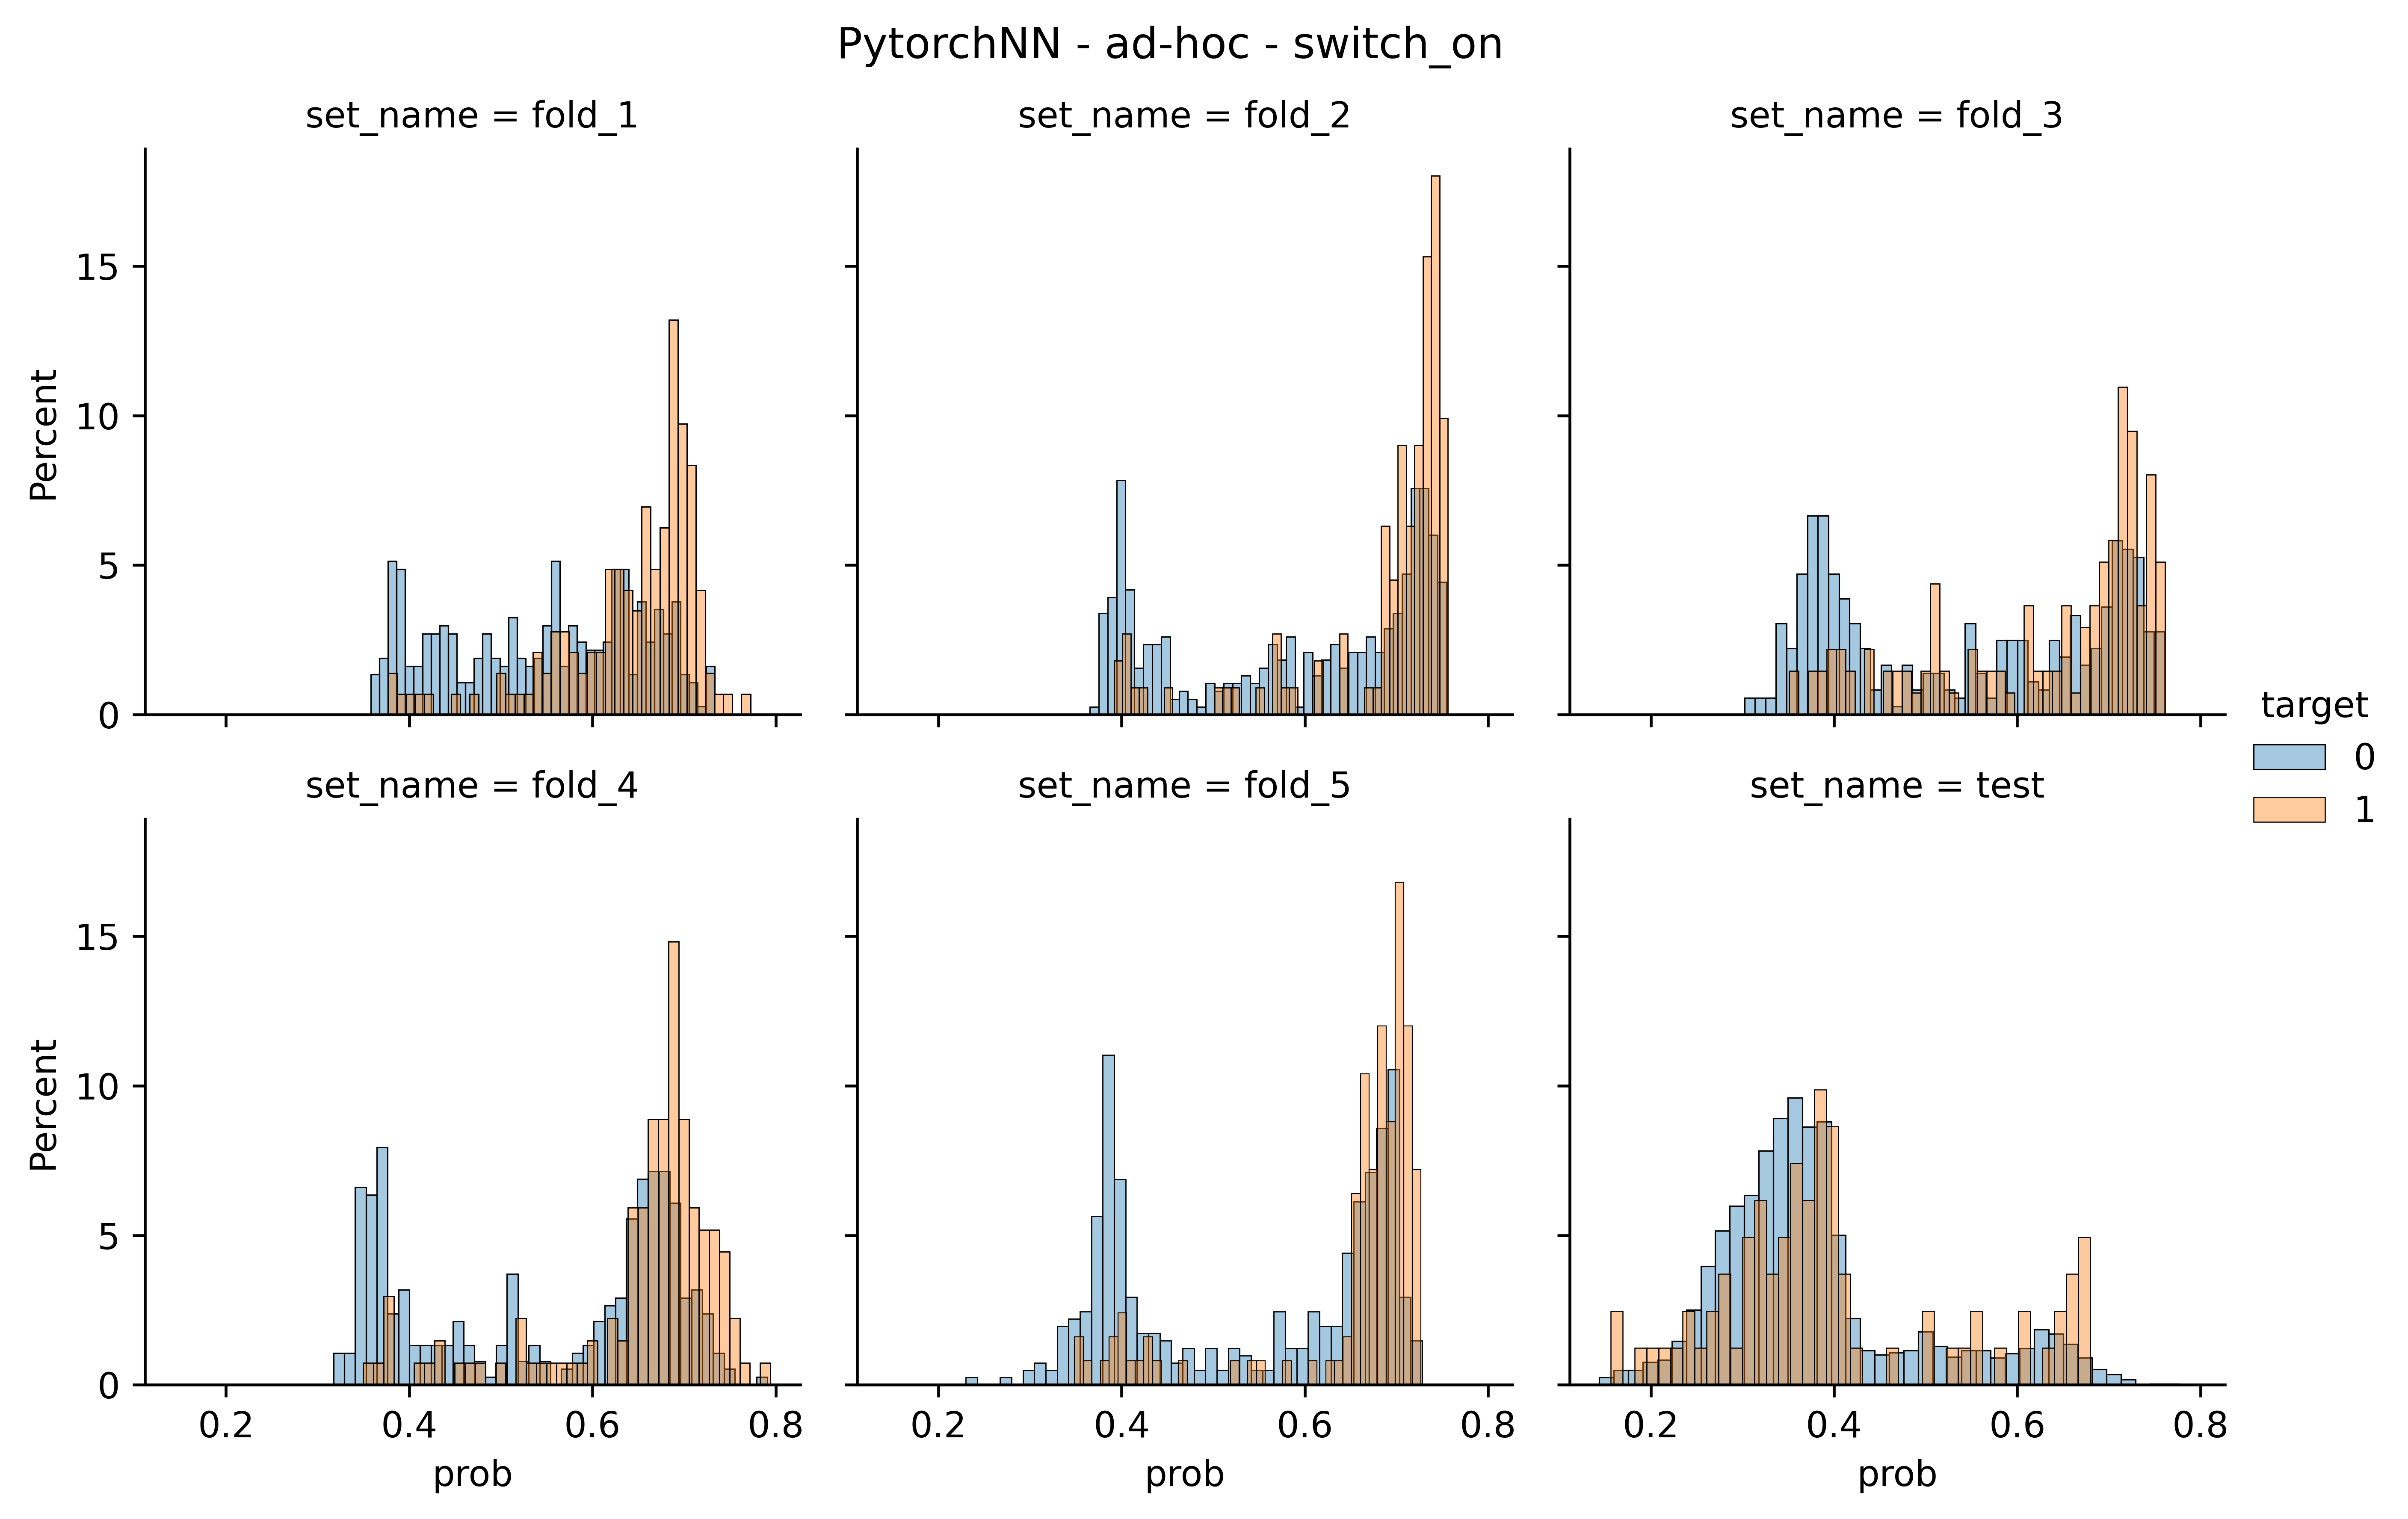
\includegraphics[width=\linewidth]{figures/results/ad-hoc/nn/switch_on/2021-12-06_18.44.35.478500__distplot.png}
    \end{subfigure}
    \caption{Ad-hoc switch\_on}
\end{figure}

\begin{figure}
    \centering
    \begin{subfigure}[b]{0.83\textwidth}
    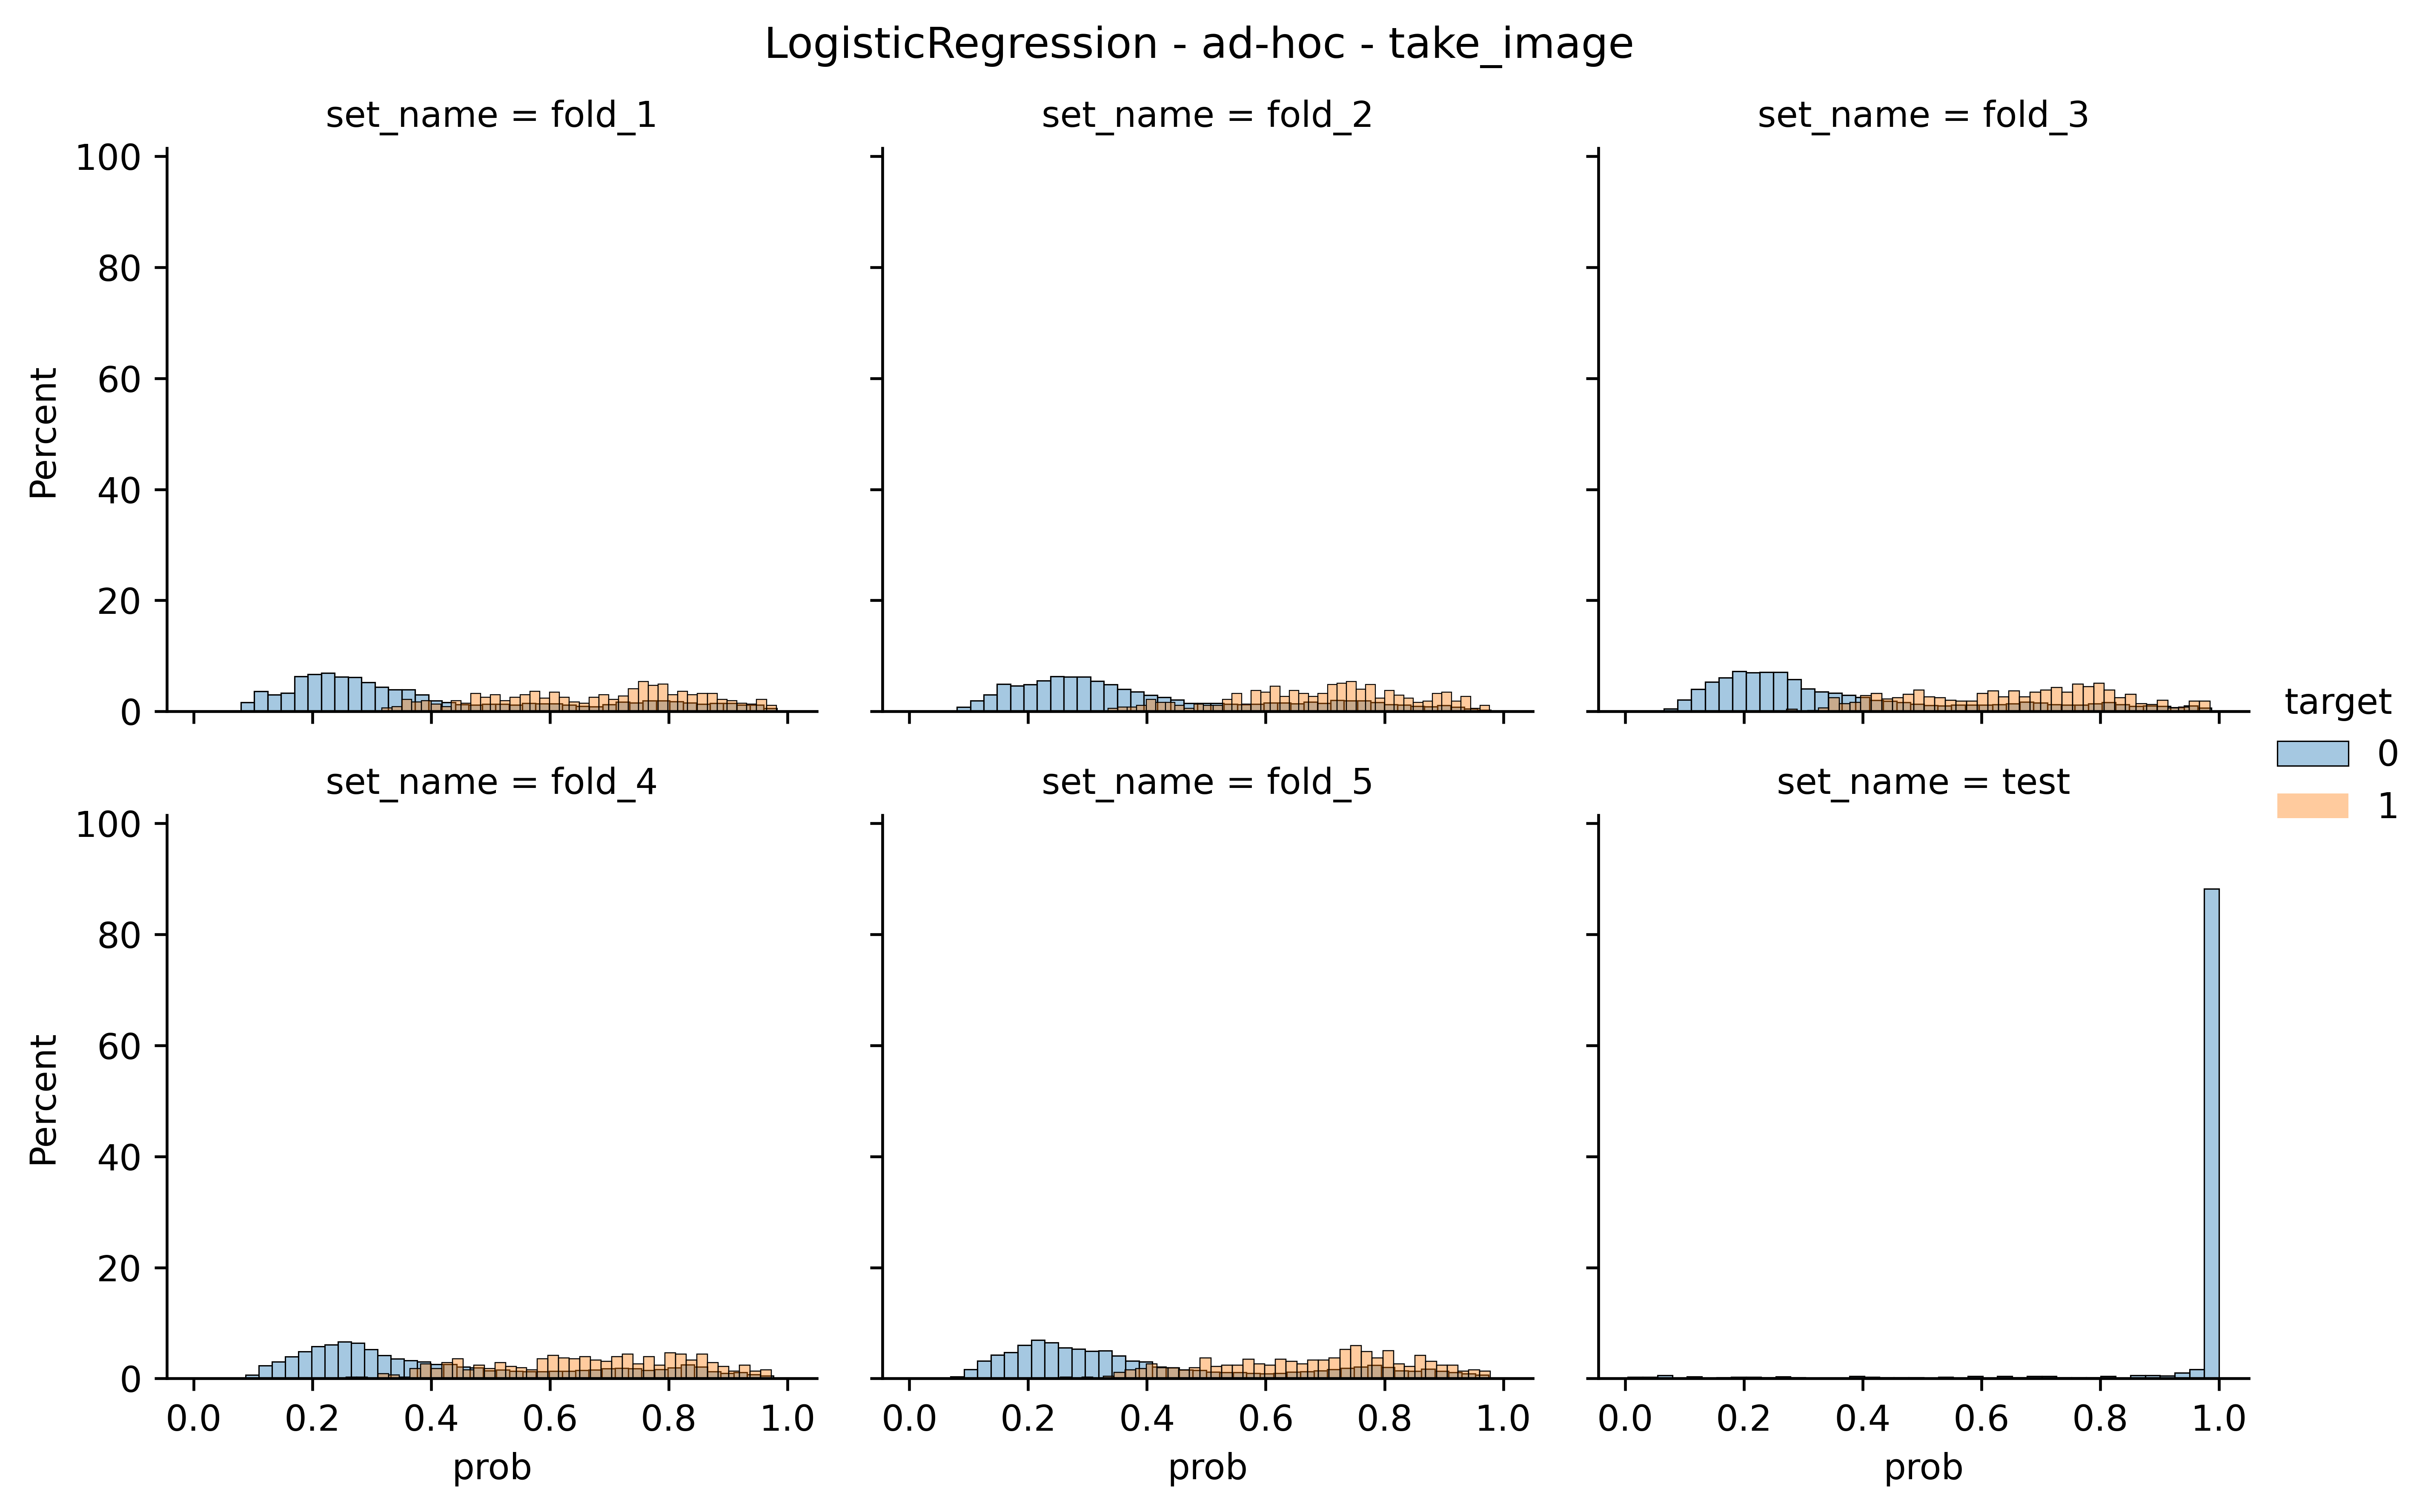
\includegraphics[width=\linewidth]{figures/results/ad-hoc/lgr/take_image/take_image__distplot.png}
    \end{subfigure}
    \hfill
    \centering
    \begin{subfigure}[b]{0.83\textwidth}
        \centering
        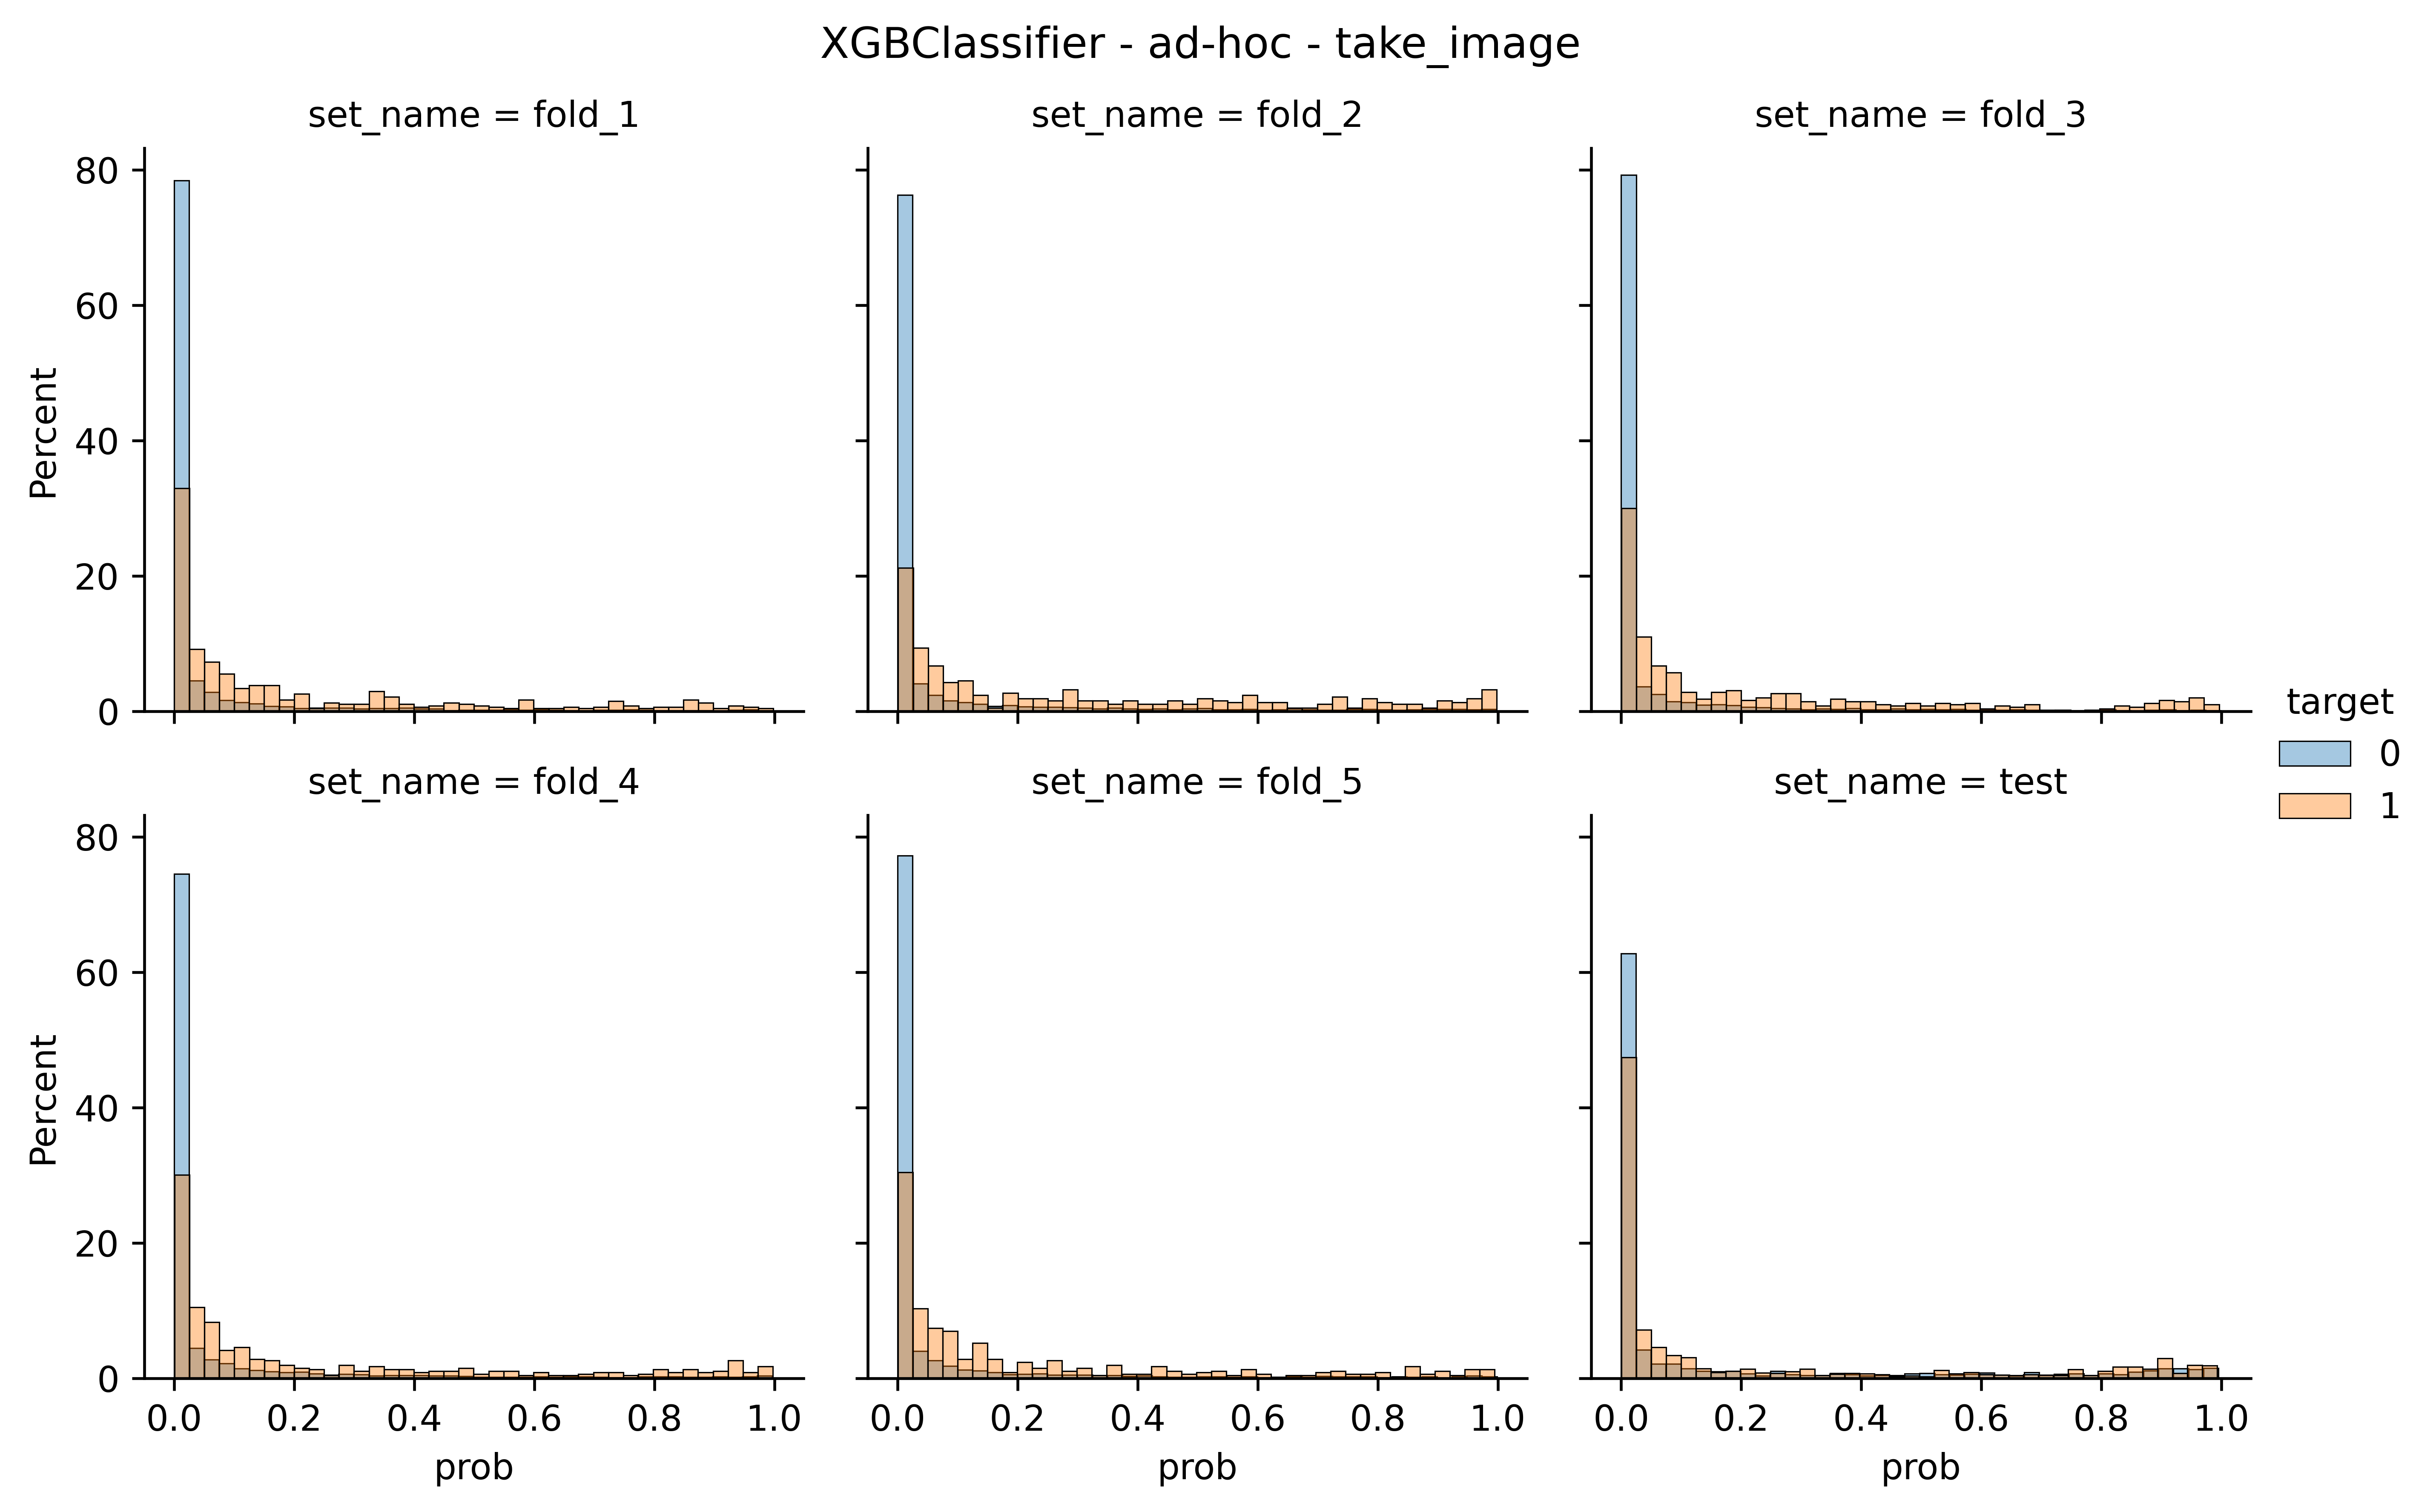
\includegraphics[width=\linewidth]{figures/results/ad-hoc/xgb/2021-12-07_07.38.35.967776__distplot.png}
    \end{subfigure}
    \caption{Ad-hoc take\_image}
\end{figure}

\section{Comparación de mejores modelos}
\label{results:comparison}

\section{Tiempos de predicción}
\label{exp:time}

Para un nuevo ejemplo no visto se debe realizar el proceso completo creación de
ventanas, codificación, predicción por parte del clasificador, y posterior
agrupamiento de ventanas para obtener la máxima prioridad. Al incluir los
modelos predictivos en el proceso de grounding heurístico el tiempo necesario
para realizar todas las etapas y obtener el valor de salida del modelo
predictivo es importante durante el proceso de grounding heurístico ya que los
planificadores deben encontrar la solución a la tarea asignada de acuerdo a un
tiempo límite, si este es excedido, ocurre una falla por parte del planificador.
Esto motivo la medición del tiempo de respuesta para los modelos predictivos
comparados en la sección \ref{results:comparison}.

Actualmente la implementación de grounding heurístico en Fast Downward, son
realizadas a nivel de ejemplo. Por lo que la unidad de medida utilizada fueron
\emph{ns/ejemplo}, no obstante también se probaron realizar las predicciones a
nivel de batch con el de determinar que tan prometedor es incluir este cambio en
el algoritmo de grounding heurístico.

\subsection{Predicciones por batch}

\subsection{Predicciones por acción}

\section{Otros experimentos}

Los experimentos presentados en las secciones \ref{exp:ad-hoc}, \ref{exp:wb}, y
\ref{exp:time} fueron aquellos principales y los que nos enfocamos durante la
tesis. No obstante, se intentaron otras vías de análisis que llevaron a 4
experimentos con el fin de lograr aquel modelo que nos permita guiar el proceso
de grounding. A pesar de no lograr resultados concretos fueron parte importante
del trabajo y otorgaron conocimiento invaluable para involucrarse más en el
dominio del problema.

\subsection{Modelos End-to-end}

End-to-end (E2E) models refieren a sistemas complejos representados por un único
modelo neuronal profundo ensamblando las capas de preprocesamiento y como capas
intermedias del modelo. En particular, este tipo de pruebas se realizaron en una
etapa temprana de la tesis donde la idea de generar ventanas de planes relajados
aún no se había investigado. En particular se experimentaron con modelos E2E de
FastText donde agrega una capa neuronal más al modelo de embeddings para que
sean utilizados en clasificación. No obstante se optó por descontinuar estos
experimentos al comenzar ya que fueron experimentos prototipos donde se buscaba
verificar la factibilidad del uso de word embeddings en grounding heurístico.

\subsection{El problema de inclusión sobre planes relajados}

Otra estrategía que utilizamos durante el análisis en la generación de ventanas
de planes relajados, fue plantear el problema de clasificación binaria como uno
multiclase. En lugar de solo 2 clases, manteníamos 4 que representaban la noción
de si una acción estaba incluido en el plan relajado y si eran parte de los good
operators del problema. Es decir, una ventana de plan relajado $w$ y acción $a$
es etiquetada como:

\begin{itemize}
    \item 0: Si $a$ no es good operator y no pertenece a $w$.
    \item 1: Si $a$ no es good operator y pertenece a $w$.
    \item 2: Si $a$ es good operator y no pertenece a $w$.
    \item 3: Si $a$ es good operator y pertenece a $w$.
\end{itemize}

Luego al agrupar por ventanas y acción, consideramos como predicción final la
clase $3$ si al menos una de las ventanas predijo $3$. Caso contrario si para
alguna ventana la predicción fue $2$ predicción del agrupamiento es $2$. Y así
sucesivamente hasta la clase $0$.

\subsection{Mayorización}

La repetición de ejemplos con etiquetas diferentes puede dificultar el
aprendizaje de un modelo, si no son preprocesadas con alguna técnica de
mayorización. Es decir, de entre todas las repeticiones del mismo ejemplo pero
con distintas clases, mantener una sola replica preservando la etiqueta que haya
ocurrido en mayor cantidad. Esta técnica fue aplicada para la codificación por
word embeddings, donde una hipótesis para mejorar la separación de los ejemplos
de entrenamiento fue asignar la etiqueta mayoritaria para todo los vector de
dimensión $D$ (plan relajado, acción) que estén cerca en un rango en
$\mathbb{R}^{D}$.

\subsection{Orden de ventanas como características}

Por último otra implementación que se agregó al sistema y que es un patrón
configurable de las etapas de ejecución es la posibilidad de mantener el orden
en que ocurren las ventanas. Es decir, se tiene

\begin{table}[h!]
\centering
\scalebox{0.9}{
 \begin{tabular}{||c | c | c | c||} 
 \hline
 Plan relajado & Orden de ventana & Acción & Etiqueta \\ [0.5ex] \hline\hline
 %(take_image satellite0 planet5 instrument1 image1)
 {}[] & 1 &{}[] & 1 \\
 {}[] & 2 &{}[] & 1 \\
 {}[] & 3 &{}[] & 1  \\
 ... & ... & ... & ...\\ [1ex] 
 \hline
 \end{tabular}}
 \caption{Ejemplos etiquetados a partir de un plan relajado y una acción}
 \label{tb:matrix_shape}
\end{table}

El objetivo de este agregado es evitar perder la información del orden durante
la separación y se buscaba analizar si es un factor relevante para el
entrenamiento y evaluación.